%----------------------------------------------------------------------------------------
% Preambulo y Configuración
%----------------------------------------------------------------------------------------

\documentclass[
    11pt,
    spanish,
    singlespacing,
    parskip,
    headsepline,
    bookmarks=true,
    unicode=true,
    pdftoolbar=true,
    pdfmenubar=true,
    pdffitwindow=false,
    colorlinks=true,
    linkcolor=blue,
    citecolor=blue,
    urlcolor=blue
]{MastersDoctoralThesis}

\usepackage[utf8]{inputenc} % Codificación de entrada UTF-8
\usepackage[T1]{fontenc}    % Codificación de salida para caracteres especiales
\usepackage{graphicx}       % Manejo de gráficos
\usepackage{eso-pic}        % Permite agregar fondos
\usepackage{hyperref}       % Manejo de hipervínculos y marcadores

% My packages
\usepackage{nicefrac}
\usepackage{gensymb}
\usepackage{amsmath}
\usepackage{tikz}           % Diagramas vectoriales
\usetikzlibrary{shapes.geometric, arrows.meta, positioning, calc}
% \usepackage{minted}
\usepackage[shortcuts]{extdash}

% Optional styling for better readability
\lstset{
    basicstyle=\ttfamily,
    breaklines=true
}

% Redefinición de caracteres problemáticos en marcadores
\hypersetup{
    pdftitle={},
    pdfauthor={Ing. Juan Ignacio Teich},
    pdfkeywords={Inteligencia Artificial},
    pdfstartview={FitH},
    unicode=true,
    colorlinks=true,
    linkcolor=blue,
    citecolor=blue,
    urlcolor=blue
}

\pdfstringdefDisableCommands{%
  \def\texttt#1{#1}%
  \def\textbf#1{#1}%
  \def\textit#1{#1}%
  \def\"{\"}%
  \def\~{~}%
  \def\'{'}%
  \def\^{}%
  \def\textunderscore{\_} % Manejo del subrayado en marcadores
}

\newcommand{\cna}{CNA\=/UII}

% Definir comandos requeridos por la clase
\newcommand{\degreename}{Carrera de Especialización en Inteligencia Artificial} % Cambia según tu título
\newcommand{\univname}{Universidad de Buenos Aires} % Cambia según tu universidad
\newcommand{\keywordnames}{Palabras clave:}
\newcommand{\titlename}{Desarrollo de una herramienta predictiva de la potencia límite de canal de la Central Nuclear Atucha II entrenada con simulaciones de código de subcanales}
%----------------------------------------------------------------------------------------
% Documento Principal
%----------------------------------------------------------------------------------------

\begin{document}

% El paquete babel (idioma spanish) activa '<' y '>' como caracteres especiales
% para comillas angulares («»), lo cual entra en conflicto con la sintaxis de
% flechas de TikZ ('->', '<-'). Se desactiva ese comportamiento.
\shorthandoff{<>}

% Configuración de la portada
\posgrado{Carrera de Especialización en Inteligencia Artificial}
\keywords{Inteligencia Artificial}

% Incluir la portada desde un archivo separado
% \include{portada}
\input{portada}

% Configuración del contenido preliminar
\frontmatter % Usar numeración romana para las páginas preliminares
\pagestyle{plain} % Estilo de encabezado simple

%----------------------------------------------------------------------------------------
% Resumen
%----------------------------------------------------------------------------------------

\begin{abstract}
\addchaptertocentry{\abstractname} % Agregar resumen al índice
Se desarrolló una metodología para estimar la Potencia Límite de Canal de la Central Nuclear Atucha II, basada en redes neuronales, con tiempos de cómputo órdenes de magnitud inferiores a los códigos termohidráulicos empleados en Nucleoeléctrica Argentina S.A. Esto permite disminuir considerablemente los tiempos y costos computacionales de los cálculos termohidráulicos para las estrategias de recambio de combustibles. 

Adicionalmente, se propone una metodología novedosa para estimar el Flujo Crítico de Calor, que incorpora redes neuronales informadas por física y redes neuronales de multifidelidad. El enfoque integra datos provenientes de ensayos experimentales con geometrías simples y con la geometría del \textit{bundle} de la Central Nuclear Atucha II, y ensayos numéricos. 

Para el desarrollo del trabajo se aplicaron conocimientos en redes neuronales, redes neuronales informadas por física, redes neuronales de multifidelidad, y su entrenamiento y optimización.


% Dentro del diseño termohidráulico de reactores nucleares, la Potencia Límite de Canal establece el límite al cual un canal refrigerante puede operar de manera segura. Esto lo convierte en un parámetro fundamental para el cálculo de estrategias de recambio de combustibles, y una alta eficiencia computacional y precisión en su estimación son cruciales para garantizar la operación segura de la central.

% Este trabajo evalúa dos posibles mejoras en ambas categorías. En primer lugar, se presenta una metodología para la estimación de la Potencia Límite de Canal con redes neuronales, entrenadas con datos de simulaciones de código de subcanales, que permiten la evaluación de estados del reactor en instantes. En segundo lugar, se propone un método novedoso para estimar el Flujo Crítico de Calor, un parámetro fundamental para la estimación de la Potencia Límite de Canal, a partir de datos de variada fidelidad: datos experimentales de ensayos con la geometría específica del combustible de la Central Nuclear Atucha II, simulaciones de códigos de subcanales con la misma geometría y las metodologías vigentes de estimación de Flujo Crítico de Calor, y datos experimentales de geometrías sencillas. Esta metodología se combina con Redes Neuronales Informadas por Física, para asegurar predicciones físicamente válidas, lo cual es fundamental en la industria nuclear.
\end{abstract}

%----------------------------------------------------------------------------------------
% Agradecimientos
%----------------------------------------------------------------------------------------

\begin{acknowledgements}
\vspace{1.5cm}
Esta sección es para agradecimientos personales y es totalmente \textbf{OPCIONAL}.
\end{acknowledgements}

%----------------------------------------------------------------------------------------
% Índice
%----------------------------------------------------------------------------------------

\tableofcontents
\listoffigures
\listoftables

%----------------------------------------------------------------------------------------
% Dedicatoria
%----------------------------------------------------------------------------------------

\dedicatory{\textbf{Dedicado a... [OPCIONAL]}}

%----------------------------------------------------------------------------------------
% Capítulos
%----------------------------------------------------------------------------------------

\mainmatter % Iniciar numeración numérica para el contenido principal
\pagestyle{thesis} % Estilo de encabezado de tesis

% Incluir capítulos desde archivos separados
% Chapter 1

\chapter{Introducción general} % Main chapter title

\label{Chapter1} % For referencing the chapter elsewhere, use \ref{Chapter1} 
\label{IntroGeneral}

A continuación, se presentan los lineamientos básicos en cuanto al funcionamiento de la Central Nuclear Atucha II, el diseño termohidráulico de la misma, y los métodos de cálculo de Potencia Límite de Canal y estimación de Flujo Crítico de Calor.

\section{Contexto y motivación}
Uno de los cálculos más importantes en el diseño termohidráulico de un reactor PHWR (del inglés, \textit{Pressurized Heavy Water Reactor}) es el de las Potencias Límite de Canal (PLC). Este cálculo puede necesitar repetirse más de un millón de veces durante cada iteración del cálculo de una estrategia de recambio de combustibles, lo que implica un alto costo computacional. Por lo tanto, obtener una herramienta que permita computar de manera eficiente las PLC e identificar los casos más críticos a ser evaluados con los códigos termohidráulicos, es de alto interés.

Adicionalmente, en el cálculo con los códigos termohidráulicos, un paso fundamental es la estimación del Flujo Crítico de Calor (CHF, del inglés \textit{Critical Heat Flux}) en función de las condiciones locales del fluido. Hoy en día, esto se realiza con métodos que se dividen en dos: fórmulas semi-empíricas que buscan capturar la alta dimensionalidad del problema, y tablas de Flujo Crítico de Calor obtenidas de ensayos en geometrías simples que luego son modificadas por factores ad-hoc para replicar lo mejor posible los ensayos realizados sobre las geometrías reales del canal refrigerante del reactor.

\section{Central Nuclear Atucha II}
La Central Nuclear Atucha II (CNA-UII) se ubica en la localidad de Lima, en la provincia de Buenos Aires, Argentina. Es una central nuclear de tipo PHWR, que utiliza agua pesada (óxido de deuterio) como moderador y refrigerante, y uranio natural como combustible. El reactor nuclear genera 2175 MW térmicos, proveyendo 745 MW eléctricos al Sistema Argentino de Interconexión (SADI). En la Figura \ref{fig:cna2} se aprecia una foto aérea de la central.

La CNA-UII comenzó su construcción en 1982, pero debido a diversos factores fue suspendida en 1994. En 2006, la empresa Nucleoeléctrica Argentina S.A. (NASA) retomó la construcción de la central, logrando su primer criticidad el 3 de junio de 2014, y finalmente obteniendo en 2016 su licencia de operación comercial. El diseño de la CNA-UII es similar al de la Central Nuclear Atucha I (CNA-UI), emplazada en el mismo predio, desarrollado originalmente por la empresa alemana Siemens-KWU.

\begin{figure}[htbp]
	\centering
	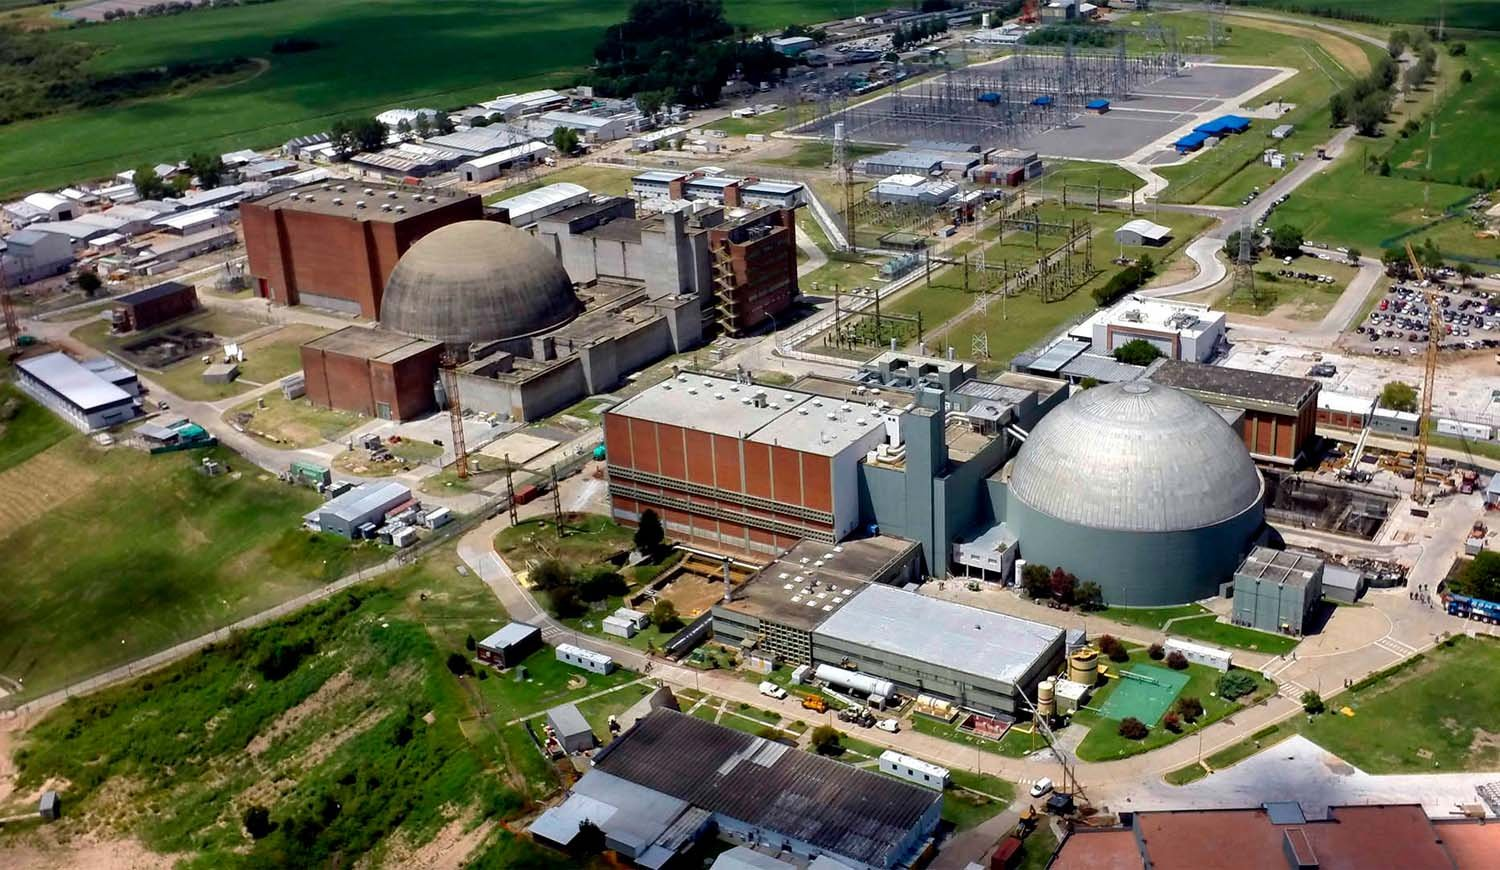
\includegraphics[width=.6\textwidth]{./Figures/cna2_aerea.jpg}
	\caption{Fotografía aérea de la Central Nuclear Atucha II.}
	\label{fig:cna2}
\end{figure}

\section{Diseño Termohidráulico de la Central Nuclear Atucha II}
El diseño termohidráulico de la CNA-UII tiene por objetivo "proporcionar una adecuada transferencia de calor compatible con la tasa de generación de calor en el núcleo y, con la capacidad de remover calor del sistema refrigerante del reactor. Además de los datos principales para el sistema refrigerante del reactor (geometría, caudal másico, nivel de presión y temperatura), el diseño termohidráulico especifica la configuración para los sistemas de control, limitación y protección del reactor que aseguran una operación segura de la planta dentro de los límites aceptables", según lo establecido en el Informe Final de Seguridad (IFS) de la CNA-UII \citep{IFS_CNA2}.

En la Tabla \ref{tab:condiciones_operacion_cna2} se presentan los principales parámetros de diseño y condiciones de operación de la CNA-UII. Se tiene un reactor con 451 elementos combustibles, cada uno alojado en un canal refrigerante, el cual toma agua pesada del plenum inferior, la calienta removiendo calor de los combustibles, y la retorna al circuito primario en el plenum superior. El núcleo se encuentra dividido en 5 zonas hidráulicas, cada una con un caudal másico característico, dado por un restrictor de caudal distintivo para cada zona de 1 a 4. La zona 5 no tiene restricción de caudal. Esta división en zonas hidráulicas se realizó con el criterio de obtener un salto entálpico uniforme en el núcleo, por lo que las zonas periféricas con menor potencia reciben menor caudal. En la Figura \ref{fig:zonas_hidraulicas} se presenta una imagen esquemática de la distribución de los canales en el núcleo de la CNA-UII, y las zonas hidráulicas del mismo.

\begin{table}[h]
	\centering
	\caption{Principales parámetros de diseño y condiciones de operación de la Central Nuclear Atucha II. \citep{IFS_CNA2}}
	\begin{tabular}{l c}    
        \toprule
        \textbf{Condiciones Generales de Operación} & \textbf{CNA-UII} \\
        \hline
        Potencia térmica del reactor & 2160 $\text{MW}_\text{th}$ \\
        Caudal másico total & 10576 $\nicefrac{\text{kg}}{\text{s}}$ \\
        Presión del Sistema Primario & 115 bar \\
        Temperatura de entrada del refrigerante & 277.8 $\degree\text{C}$ \\
        Temperatura de salida del refrigerante & 314.6 $\degree\text{C}$ \\
        Cantidad de zonas hidráulicas del núcleo & 5 \\
        Cantidad de elementos combustibles en el núcleo & 451 \\
        Cantidad de barras combustibles por elemento combustible & 37 \\
		\bottomrule
		% \hline
	\end{tabular}
	\label{tab:condiciones_operacion_cna2}
\end{table}

\begin{figure}[htbp]
	\centering
	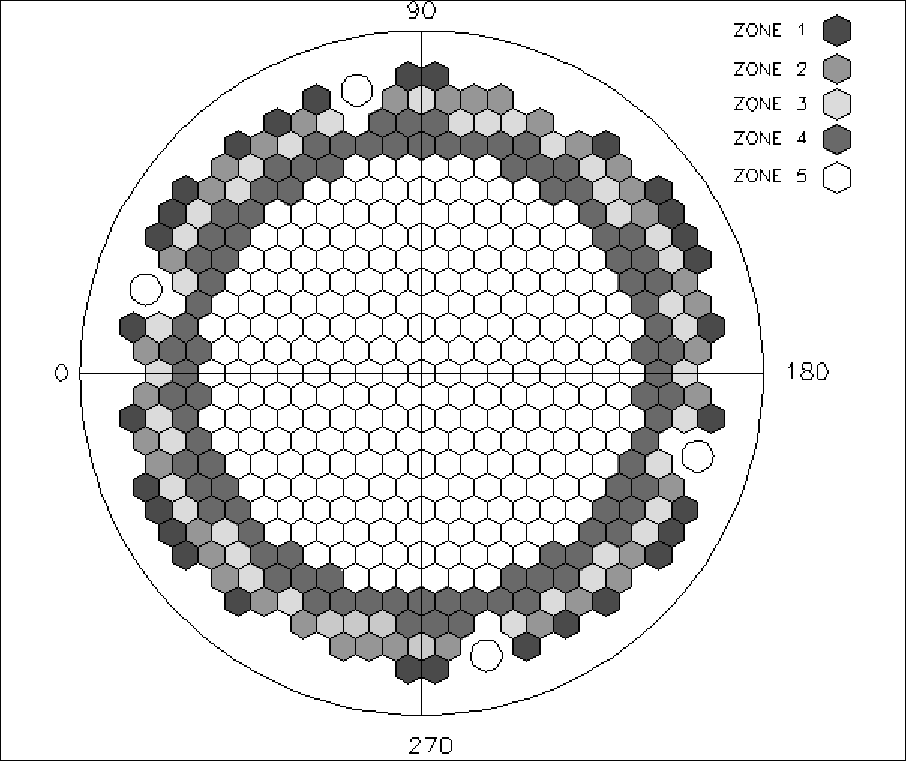
\includegraphics[width=.6\textwidth]{./Figures/zonas_hidraulicas.png}
	\caption{Esquematización de los canales refrigerantes en el núcleo de la CNA-UII y las 5 zonas hidráulicas. \citep{IFS_CNA2}}
	\label{fig:zonas_hidraulicas}
\end{figure}

Para cumplir con los criterios de diseño y operación segura establecidos en el IFS, se deben cumplir dos principales criterios en cuanto a la potencia a la que pueden operar los combustibles dentro del núcleo: el criterio de límite de vacío a la salida de los canales refrigerantes y el criterio de Apartamiento de la Ebullición Nucleada (DNB, del inglés \textit{Departure from Nucleate Boiling}).

En primer lugar, la fracción de vacío ($\alpha$) se define como el porcentaje del área a la salida del canal ocupada por vapor:
\begin{equation}
    \alpha = \frac{A_\text{vapor}}{A_\text{vapor} + A_\text{líquido}},
\end{equation}
y tiene un límite autoimpuesto para evitar vibraciones excesivas en los elementos combustibles y los componentes que aseguran su rigidez estructural. La fracción de vacío está relacionada con el título termodinámico ($x$) de la mezcla de vapor y líquido por la siguiente ecuación:
\begin{equation}
    \alpha = \cfrac{1}{1 + \cfrac{1-x}{x}\cdot \cfrac{\rho_v}{\rho_l}\cdot S},
\end{equation}
siendo $S$ el \textit{slip ratio}, definido como el cociente entre la velocidad del vapor y la velocidad del líquido:
\begin{equation}
    S = \frac{v_v}{v_l}.
\end{equation}

El límite por DNB se explica en la siguiente sección.

\section{Apartamiento de la Ebullición Nucleada (DNB)}

Para poder explicar el fenómeno de DNB, primero se debe introducir el régimen de flujo típico de un reactor de tipo PHWR. En este tipo de reactores el fluido refrigerante se encuentra subenfriado a la entrada del canal refrigerante, y a medida que asciende por el mismo puede transicionar a un régimen de ebullición nucleada, donde se forman burbujas de vapor en la superficie de las vainas combustibles. 

La ebullición nucleada es un régimen de transferencia de calor muy eficiente, ya que las burbujas que se forman en la superficie facilitan la transferencia de calor al líquido. En la Figura \ref{fig:nukiyama} se puede observar la curva de Nukiyama \citep{NUKIYAMA1966}, que representa la relación entre el flujo de calor y la diferencia entre la temperatura de pared y la temperatura de saturación del líquido, para el caso de un cable sumergido en una pileta de agua. Se observa que hasta el comienzo de la ebullición nucleada (ONB, del inglés \textit{Onset of Nucleate Boiling}), el flujo aumenta con la diferencia de temperatura. Luego del ONB, la pendiente se incrementa, es decir, que aumenta la capacidad de transferencia de calor. Sin embargo, este incremento tiene un límite, el punto B de la curva o CHF. En ese punto se tiene un salto repentino al punto D, donde la temperatura de pared aumenta drásticamente, entrando en un régimen de ebullición por película, donde la transferencia de calor es muy ineficiente por la película de vapor que aisla la pared calefaccionada del líquido.

En la Figura \ref{fig:dnb} se tiene el mismo fenómeno, pero representado en un tubo cuyas paredes están calefaccionadas, al cual ingresa líquido por la parte inferior. Se observa que al ascender el régimen pasa de transferencia por convección al líquido subenfriado, a ebullición subenfriada (es decir, con temperatura promedio del líquido por debajo de la temperatura de saturación), a ebullición nucleada en saturación, y finalmente al apartamiento de la ebullición nucleada y la ebullición en película.

El criterio de seguridad del diseño termohidráulico de una central es garantizar la integridad las vainas combustibles y las pastillas de combustible dentro de las mismas. Para esto, se requiere que la temperatura de las mismas esté por debajo de un cierto valor establecido en el diseño. Si retornamos a la curva de Nukiyama (Figura \ref{fig:nukiyama}), podemos comprender que evitar el DNB es entonces un principio fundamental en el diseño termohidráulico de un reactor PHWR. 

\begin{figure}[htbp]
	\centering
	% 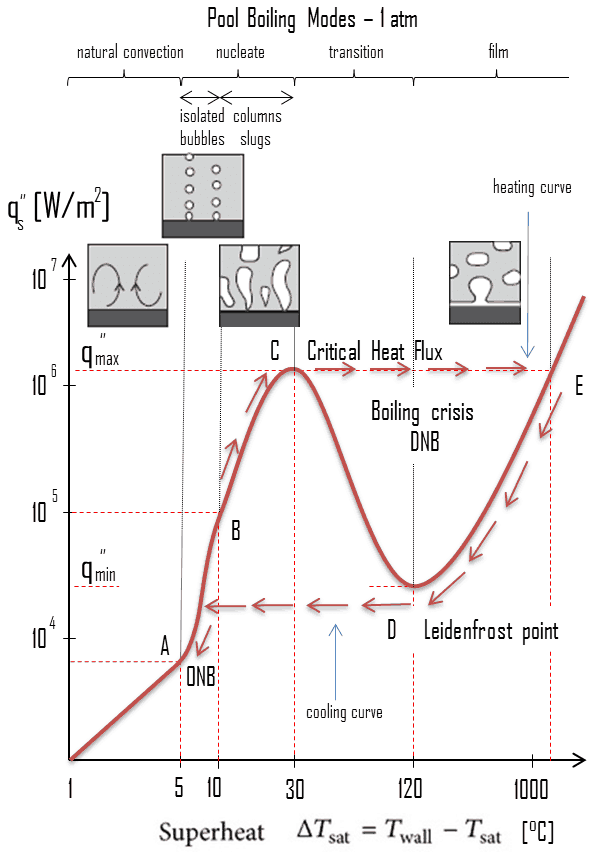
\includegraphics[width=.6\textwidth]{./Figures/curva_nukiyama.png}
	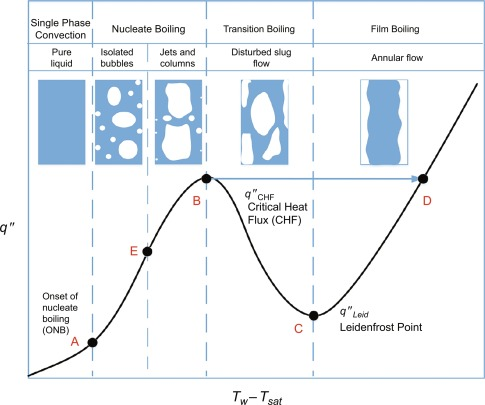
\includegraphics[width=.8\textwidth]{./Figures/nukiyama.jpg}
	\caption{Curva de Nukiyama.}
	\label{fig:nukiyama}
\end{figure}

\begin{figure}[htbp]
	\centering
	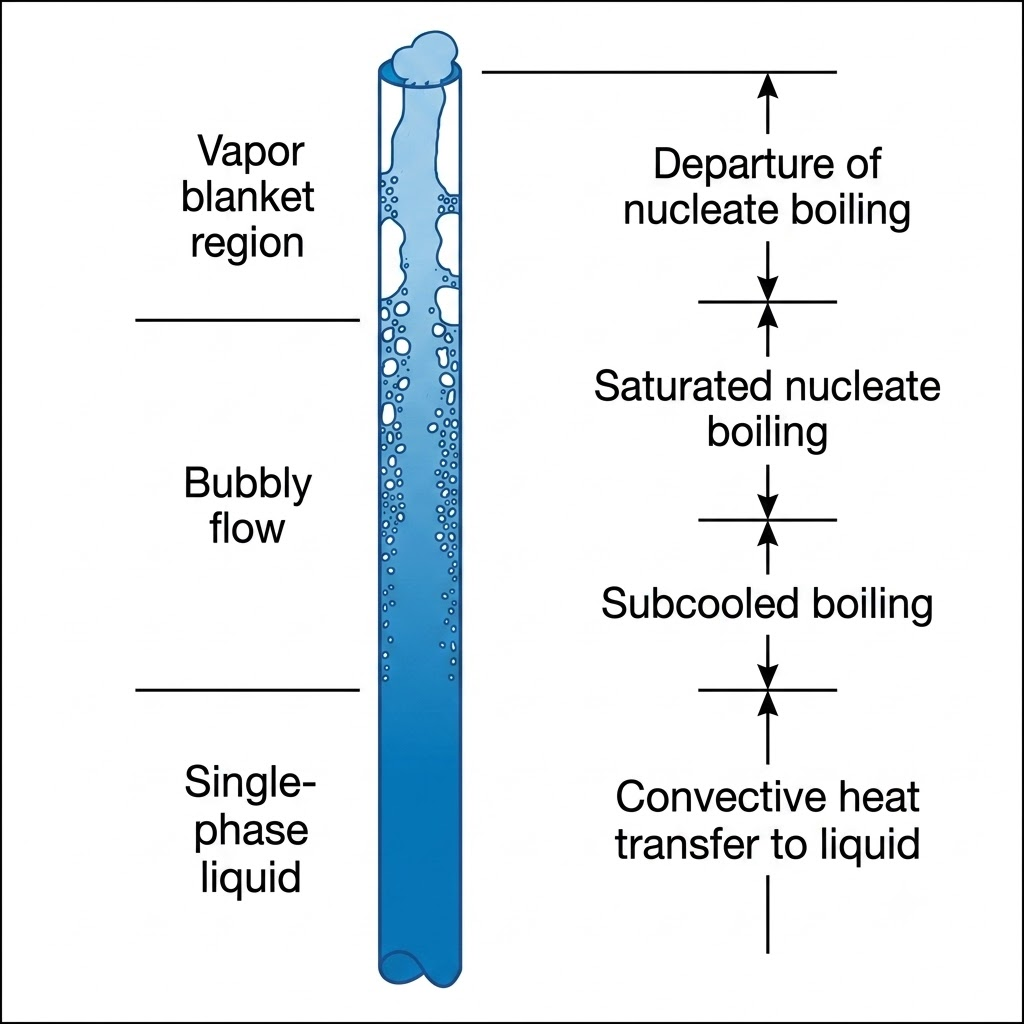
\includegraphics[width=.7\textwidth]{./Figures/dnb.jpg}
	\caption{Esquematización del Apartamiento de la Ebullición Nucleada (DNB) en un tubo.}
	\label{fig:dnb}
\end{figure}

\section{Cálculo de Potencia Límite de Canal}
Se tiene entonces dos límites relacionados a la potencia a la que puede operar un canal refrigerante: por fracción de vacío y por DNB. El cálculo de la Potencia Límite de Canal (PLC) consiste en determinar la potencia máxima a la que puede operar un canal refrigerante sin superar los límites de fracción de vacío y DNB.

Para tener en cuenta la incerteza en la estimación del CHF, la sensibilidad de ésta con respecto a las condiciones de operación del núcleo, y que todos los transitorios operacionales previstos deben cumplir con asegurar que no se tenga DNB, se debe plantea asegurar un márgen al DNB o DNBR (del inglés, \textit{Departure from Nucleate Boiling Ratio}). Entonces, la PLC por DNB en rigor es aquela potencia a la cual se mantiene el DNBR establecido en el IFS de la CNA-UII, el cual es característico para cada zona hidráulica.

El cálculo de las PLC para la CNA-UII se realiza utilizando dos códigos termohidráulicos. En primer lugar se utiliza el código COBRA3-CP \citep{cobra3cp}, un código de subcanales desarrollado originalmente por el MIT, modificado posteriormente por la empresa alemana Siemens-KWU en los años ochenta, y luego por INVAP en el año 2008. Estas modificaciones han permitido adaptar el código, pensado originalmente para reactores de tipo PWR, a la geometría específica del reactor de la CNA-UII. El código COBRA-3CP permite simular el comportamiento termohidráulico de un canal refrigerante, y determinar la potencia a la que se alcanza el límite por vacío y el límite por DNB.

Por otro lado, el código AXCNA \citep{axcna}, de desarrollo interno de la Gerencia de Análisis de Seguridad y Diseño del Núcleo (GASyDN) de NASA, permite simular el comportamiento hidráulico de todo el sistema primario para obtener la pérdida de carga en el reactor, a partir de la señal de salto de presión en las bombas del primario. Luego, se utiliza este valor para calcular la distribución de caudal entre los canales refrigerantes, en función de los restrictores de caudal y las pérdidas hidráulicas por la generación de vapor en los canales. Esto permite estimar en tiempo real el límite al DNB de cada canal refrigerante, y, en conjunto con los medidores de potencia in-core, provee al sistema de limitación de potencia (RELEB, del alemán \textit{Reaktor LeistungsBegrenzung}) la información necesaria para computar el márgen de potencia en tiempo real.

Las PLC también son utilizadas para el cómputo de las estrategias de recambios de combustibles, teniendo un proceso iterativo entre el cómputo neutrónico de las estrategias y el recálculo termohidráulico de las PLC. Por lo tanto, es de interés tener un método rápido y confiable para evaluar las estrategias de recambio, e identificar los estados del reactor más comprometido dentro de las mismas para su análisis detallado con AXCNA y COBRA3-CP.

\subsection{Códigos de subcanales}
A continuación se desarrolla la teoría base del método de los códigos de subcanales, utilizando como base el Manual de Modelos de COBRA3-CP \citep{cobra3cp}.

En la Figura \ref{fig:sch} se esquematiza la discretización en subcanales. Esta busca generar elementos prismáticos, los cuales tienen algunas caras en contacto con las vainas combustibles, y otras en contacto con subcanales adyacentes. De esta forma, se puede resolver por medio de las ecuaciones de conservación en su formato unidimensional, y sólo es necesario agregar una componente transversal debido a la comunicación entre subcanales y una ecuación de conservación para la cantidad de movimiento transversal.

\begin{figure}[htbp]
	\centering
	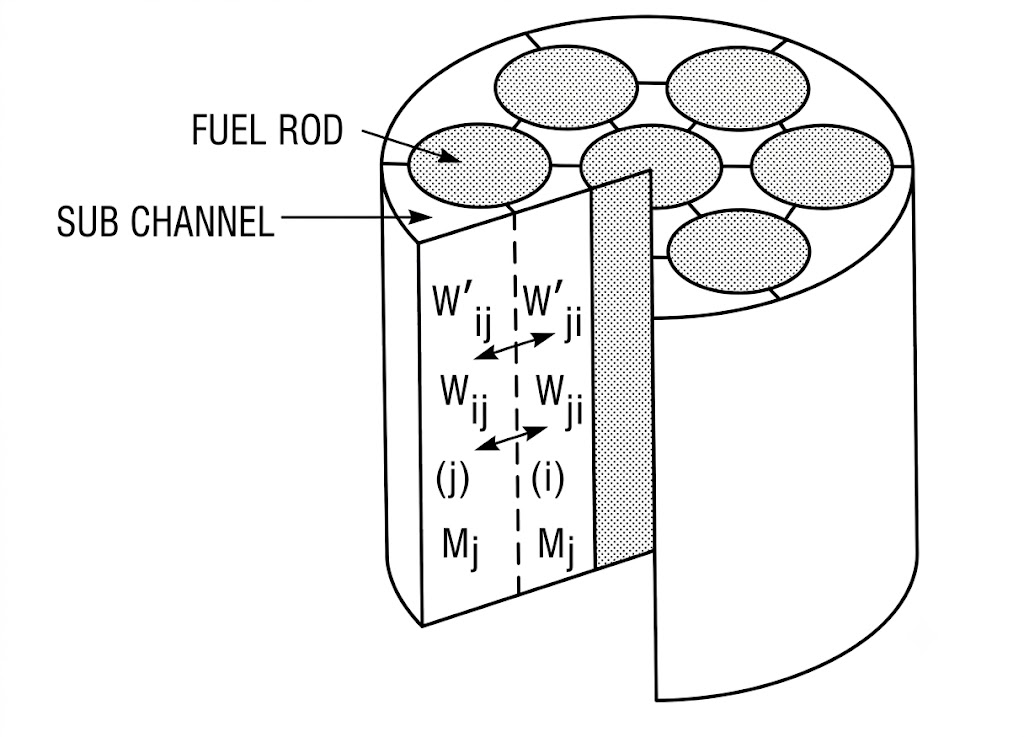
\includegraphics[width=.6\textwidth]{./Figures/subchannels.jpg}
	\caption{Esquematización de discretización en subcanales. Obtenido del Manual de Modelos de COBRA3-CP \citep{cobra3cp}}
	\label{fig:sch}
\end{figure}

Entonces se desarrollan las ecuaciones de conservación para un dado subcanal $i$ a continuación. En primer lugar, la conservación de la masa viene dada por:

\begin{equation}
    A \frac{\partial \rho_i}{\partial t} + \frac{\partial \dot{m}_i}{\partial z} + \sum_j w_{ij} = 0,
\end{equation}
siendo $A$ el área de paso, $\rho$ la densidad, $\dot{m}$ el caudal másico, $z$ la coordenada axial y $w_{ij}$ el factor de flujo cruzado por diversión.

Luego, se presenta la conservación de la energía:
\begin{equation}
    A \frac{\partial (\rho h)_i}{\partial t} + \frac{\partial (\dot{m} h)_i}{\partial z} = q'_i - \sum_j w^{*H}_{ij} (h_i - h_j) - \sum_j w_{ij} h^* + A \frac{Dp}{Dt},
\end{equation}
siendo $h$ la entalpía, $q'$ el flujo de calor, $w^{*H}_{ij}$ el factor de flujo cruzado efectivo por transporte de energía, $h^*$ la entalpía transportada por diversión y $p$ la presión.

En tercer lugar, se tiene la conservación de la cantidad de movimiento axial:
\begin{equation}
    \frac{\partial \dot{m}_i}{\partial t} + \sum_j w_{ij} u^*_j + \frac{\partial (\dot{m} u_z)_i}{\partial z} = -A \rho g_z - A \frac{\partial p}{\partial z} - \sum_j w^{*M}_{ij} (u_{zi} - u_{zj}) - F_{iz},
\end{equation}
siendo $u^*$ la velocidad axial transportada por diversión, $u$ la velocidad con subíndice según la dirección, $g_z$ la aceleración de la gravedad, $w^{*M}_{ij}$ el factor de flujo cruzado efectivo por transporte de momento y $F_i$ la fuerza de arrastre por fricción y forma con subíndice según la dirección.

Por último, la conservación de la cantidad de movimiento transversal viene dada por:
\begin{equation}
    \frac{\partial w_{ij}}{\partial t} + \frac{\partial w_{ij} u_x}{\partial x} + \frac{\partial w_{ij} u_z}{\partial x} = - s_{ij} \frac{\partial p}{\partial x} - F_{ix}.
\end{equation}

Es importante notar que los términos de flujo cruzado son de carácter empírico, y para su determinación se utilizan ensayos de mezclado en condiciones subenfriadas para la geometría específica que se quiere modelar. Estos términos han sido determinados de esta forma para el \textit{bundle} de la CNA-UII, y se continúan proponiendo mejoras para su modelado.
\chapter{Introducción específica} % Main chapter title
\label{Chapter2}

A continuación, se explican los frameworks, arquitecturas y bibliotecas utilizadas en el trabajo, los conjuntos de datos utilizados para el entrenamiento y validación de los modelos, y por último, una breve mención a la infraestructura de cómputo utilizada. 

\section{Frameworks y bibliotecas}

Las Redes Neuronales Profundas (DNN, del inglés \textit{Deep Neural Networks}) son el modelo fundamental de Aprendizaje Profundo. El objetivo de una DNN es aproximar una función $f^*$, definiendo un mapeo $\mathbf{y}=f(\mathbf{x};\mathbf{\theta})$ del cual se aprenden los parámetros $\mathbf{\theta}$ para lograr la mejor aproximación de la función objetivo. La unidad básica de las DNN es el perceptrón, el cual aplica una transformación lineal seguido de una transformación no-lineal, llamada activación. Decimos redes neuronales, debido a que se aplican múltiples perceptrones en capas consecutivas. Podemos pensar a las DNN como "máquinas de aproximación de funciones, diseñadas para obtener generalización estadísitica" \citep{GOODFELLOW_DEEPLEARNING}. Esto las hace interesantes para su aplicación en la resolución del primer problema planteado en este trabajo: la estimación rápida de PLC, aprovechando la basta cantidad de datos acumulados.

También es de interés en este trabajo analizar la aplicación de reducción de dimensionalidad a partir de algunos \textit{set} de \textit{features}. Para realizar esto, se utiliza una arquitectura \textit{encoder-decoder}. Esta arquitectura se encuentra representada en la figura \ref{fig:embedding}, donde se observa una primera DNN, llamada \textit{encoder}, que reduce de dimensión el \textit{input} al vector \textit{feature} o \textit{embedding}, y luego una segunda DNN, llamada \textit{decoder}, que reconstruye a partir del \textit{embedding} el \textit{input}. Esto permite representar la misma información con una menor dimensionalidad, capturando las características representativas del vector de entrada.

Por otro lado, para el planteo de una nueva metodología de estimación de CHF utilizando ML, nos centramos en dos arquitecturas particulares derivadas de las DNN. En el trabajo de Raissi, Perdikaris y Karniadakis \citep{RAISSI2019} se presentan las PINN, las cuales permiten obtener una función de pérdida que busque cumplir una ecuación diferencial en derivadas parciales (PDE, del inglés \textit{Partial Differential Equation}), además de la función de pérdida respecto de los datos tabulados para entrenamiento. 

En la figura \ref{fig:pinn} se presenta un esquema general de una arquitectura PINN. Se tiene una DNN que predice $\hat{u}$ a partir de las entradas $\mathbf{x}$ y $t$. Luego se computa por medio de diferenciación automática las derivadas necesarias de $\hat{u}$, como pueden ser la derivada temporal, el gradiente, el laplaciano, etc. Luego, se calcula el error cuadrático medio (MSE, del inglés \textit{Mean Squared Error}) del residuo del ajuste de los datos rotulados, el residuo de la ecuación de gobierno, el residuo de las condiciones de borde y el residuo de las condiciones iniciales, para luego computar la pérdida global y su gradiente para aplicar el algorítmo de aprendizaje basado en gradiente.

Este enfoque se puede denominar como \textit{grey box}, ya que el modelo, si bien tiene una componente desconocida al entrenarse y ajustar sus parámetros, tiene a la función de pérdida de forma conocida que nos da información de su funcionamiento interno. Los modelos de DNN típicamente se llaman \textit{black box}, mientras que modelos más tradicionales de resolución de problemas físicos como las diferencias finitas, los elementos finitos o los volúmenes finitos, son considerados modelos \textit{white box}. Esta característica es interesante para su aplicación en el ámbito nuclear, ya que este requiere de alta certeza en las predicciones debido a los altos estándares de seguridad que se deben cumplir.

Por otro lado, en el trabajo de Meng y Karniadakis \citep{MENG2020} se presenta una arquitectura novedosa de redes neuronales, llamadas Redes Neuronales Profundas de Multi-Fidelidad (MFDNN, del inglés \textit{Multi-Fidelity Deep Neural Networks}). Esta arquitectura permite considerar conjuntos de datos de distinta fidelidad, por ejemplo, datos obtenidos a partir de ensayos experimentales (alta fidelida, disponibilidad acotada o baja), datos obtenidos a partir de ensayos numéricos (baja fidelidad, disponibilidad acotada o alta), datos de ensayos experimentales en geometrías o condiciones diferentes (baja fidelidad, disponibilidad alta), etc. Para realizar esto, propone la hipótesis de que los datos de alta fidelidad tienen una relación no-lineal con los datos de baja fidelidad de la forma: 
\begin{equation}
	y_H = \mathcal{F}(\mathbf{x}, y_L),
\end{equation}
siendo $y_H$ la información de alta fidelidad, $y_L$ la información de baja fidelidad y $\mathbf{x}$ los datos de entrada. Esta relación no-lineal es posible de representar con una DNN, por lo que se construye una arquitectura que consiste de una DNN que estima $y_L$ a partir de $\mathbf{x}$, y luego otra que estima $y_H$ a partir de $\hat{y_L}$ y $\mathbf{x}$. En la figura \ref{fig:mfdnn} se esquematiza esta arquitectura. Debe notarse que el trabajo original propone estimar la relación entre alta y baja fidelidad por medio de dos redes, una lineal ($\mathcal{F}_l$) y otra no-lineal ($\mathcal{F}_{nl}$), pero esto es redundante, ya que una red no-lineal puede capturar la relación lineal.

Si agregamos una función de pérdida basada en lo propuesto en las PINN, obtenemos la variante informada por física de las MFDNN, las Redes Neuronales Informadas por Física de Multi-Fidelidad (MFPINN, del inglés \textit{Multi-Fidelity Physics-Informed Neural Networks}). Esto es lo que se representa en la figura \ref{fig:mfdnn} con el cómputo de las derivadas de $\hat{y_H}$ y el posterior cálculo de $f_e$.

Para realizar el desarrollo de las arquitecturas mencionadas, en este trabajo se utiliza la librería PyTorch \citep{PYTORCH} \citep{PYTORCH_WEBSITE}.

% \pagebreak
% \begin{equation}
% 	\text{MSE} = \text{MSE}_{y_L} + \text{MSE}_{y_H} + \text{MSE}_{f_e} + \lambda \sum \beta_i^2
% \end{equation}

\begin{figure}[htbp]
	\centering
	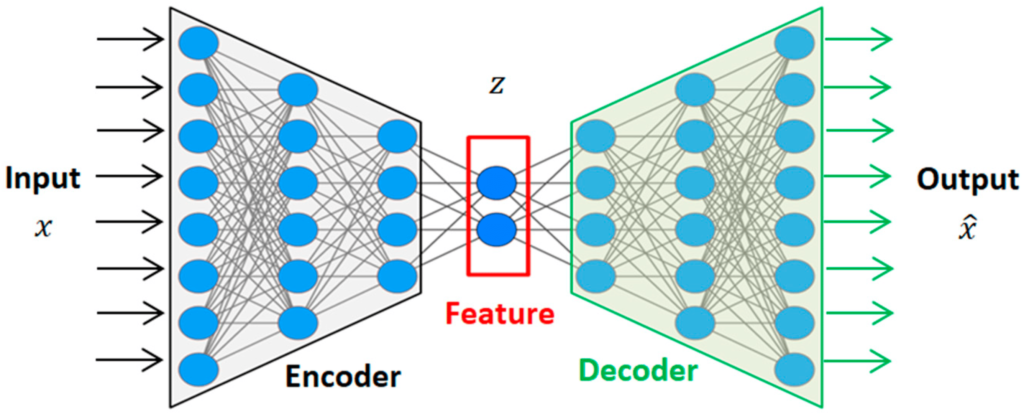
\includegraphics[width=.7\textwidth]{./Figures/encoder-decoder.png}
	\caption{Esquema de arquitectura encoder-decoder\protect\footnotemark{}.}
	\label{fig:embedding}
\end{figure}
\footnotetext{Imagen tomada de \href{https://muditb.com/neural-encoders-from-autoencoders-to-modern-retrieval-architectures/}{https://muditb.com}.}

\begin{figure}[htbp]
	\centering
	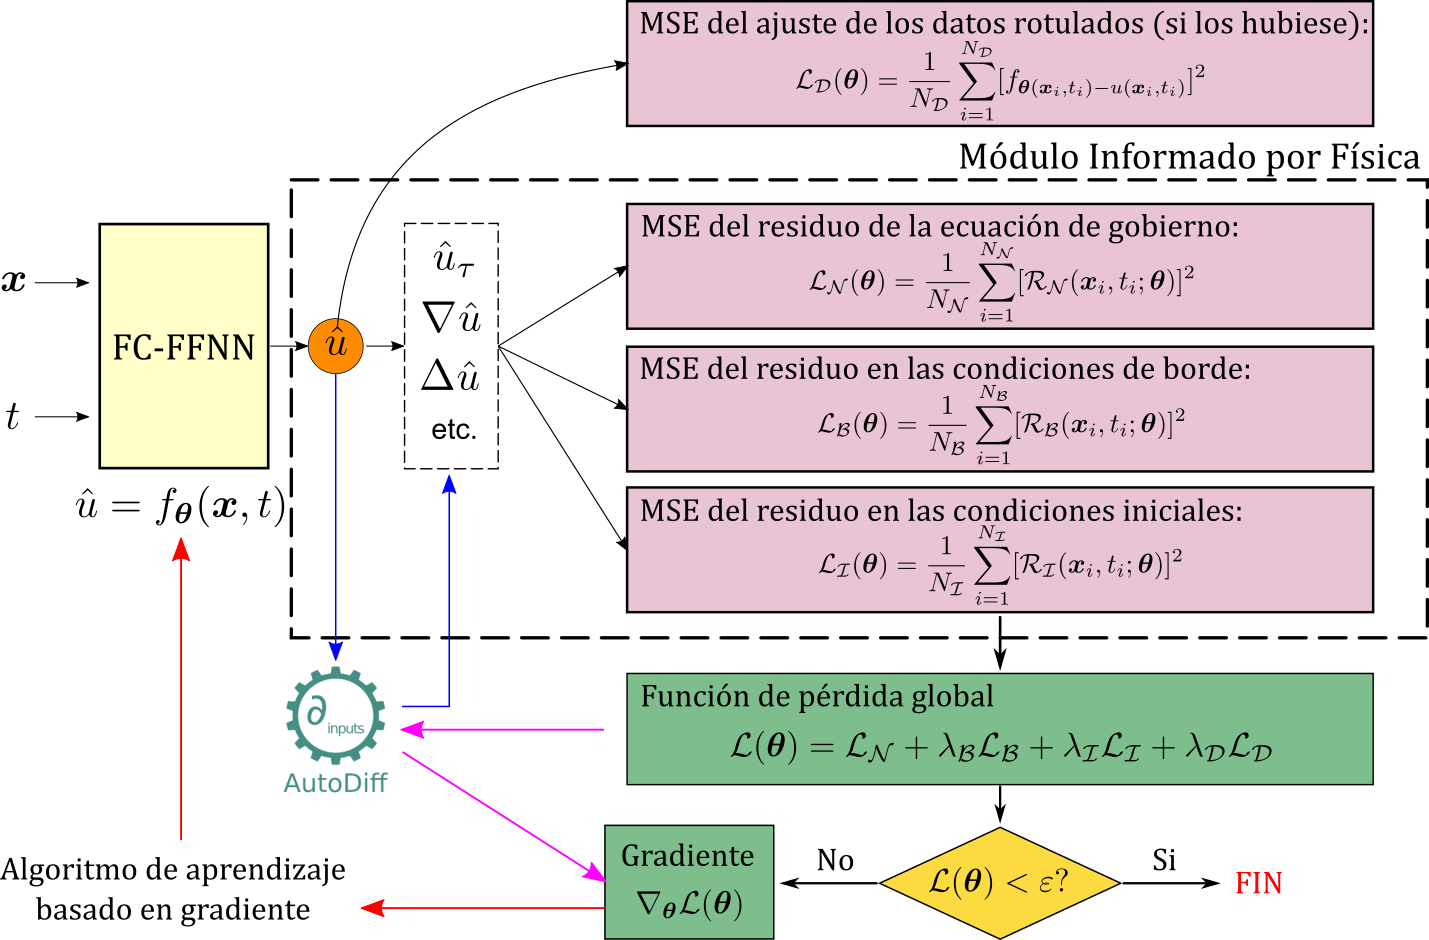
\includegraphics[width=.9\textwidth]{./Figures/pinn.png}
	\caption{Esquema de PINN\protect\footnotemark{}.}
	\label{fig:pinn}
\end{figure}
\footnotetext{Imagen tomada del curso \textit{Redes Neuronales Informadas por Física} de la CEIA.}

\begin{figure}[htbp]
	\centering
	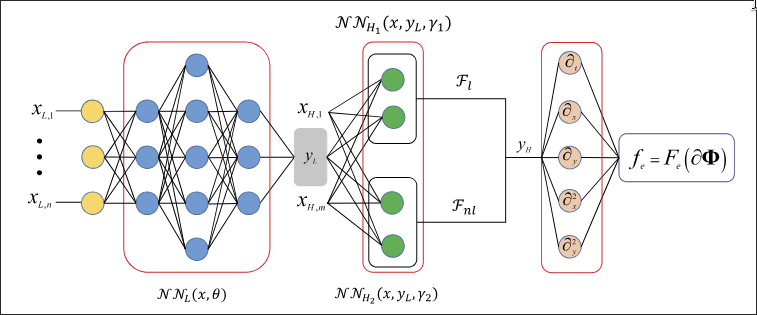
\includegraphics[width=.9\textwidth]{./Figures/mfdnn.png}
	\caption{Esquema de MFDNN y MFPINN\protect\footnotemark{}.}
	\label{fig:mfdnn}
\end{figure}
\footnotetext{Imagen tomada de Meng y Karniadakis \citep{MENG2020}.}

\pagebreak

\section{Datasets y datos de entrenamiento}

En cuanto a los datos de entrenamiento, debemos dividir esta sección en los datos utilizados para la estimación de las PLC y para la estimación de CHF.

Para la estimación de PLC, se utilizan datos de simulaciones realizadas por la División de Diseño Termohidráulico de la Gerencia de Análisis de Seguridad y Diseño del Núcleo (GASyDN) de Nucleoeléctrica Argentina S.A. (NA-SA), los cuales son de carácter confidencial. Los datos fueron generados con el código de simulación termohidráulica de subcanales COBRA3-CP \citep{cobra3cp}, a partir de estados del reactor calculados en las simulaciones de estrategias de recambio de combustibles. De las salidas de las simulaciones de COBRA3-CP se extrae:
\begin{itemize}
	\item Perfil axial de potencia.
	\item Perfil de potencia por barra combustible.
	\item Mínimo DNBR.
	\item Temperatura de entrada.
	\item Presión de salida.
	\item Potencia total.
	\item Zona hidráulica.
\end{itemize}

Por otro lado, para la estimación de CHF, se tiene múltiples fuentes de datos. Se incluyen: los datos de ensayos en un tubo usados por Groeneveld en su LUT 2006 \citep{GROENEVELD2007}, obtenidos de \citep{USNRC2019NUREGKM0011}; los datos de ensayos sobre el \textit{bundle} de la CNA-UII realizados por la Universidad de Columbia \citep{recopilacion_columbia}; y el replicado de los ensayos de Columbia con COBRA3-CP, ampliando la cantidad de puntos de ensayo. Estas últimas dos fuentes de datos son de carácter confidencial. 

Los datos de ensayos en un tubo tienen los siguientes datos disponibles: diámetro, longitud, presión a la salida, flujo másico, título termodinámico a la salida, entalpía a la entrada, flujo de calor y temperatura de entrada. 

Los datos de los ensayos de Columbia tienen los siguientes datos disponibles: presión a la salida, temperatura de entrada, flujo másico, flujo de calor, título termodinámico a la salida y diferencia de presión a la entrada.

\section{Infraestructura de cómputo}

En cuanto a infraestructura de cómputo, debido al carácter confidencial de los datos utilizados, se opta por realizar todo el proceso de entrenamiento en un entorno local. Para ello se dispone de dos computadoras, una provista por la empresa NA-SA, con una placa gráfica NVIDIA A2000 y 32GB de RAM, y otra de uso personal del autor, con una placa gráfica NVIDIA RTX 3090 y 64GB de RAM. Ambas computadoras tienen capacidad apta para el trabajo en cuestión. 
\chapter{Diseño e implementación} % Main chapter title

\label{Chapter3} 

En este capítulo se describe el diseño e implementación de los dos modelos desarrollados en este trabajo. Debido a la naturaleza del trabajo, se divide el capítulo en dos secciones, una para la estimación de PLC y otra para la de CHF.

\section{Estimación de PLC}
En esta sección se describe el modelo para estimar PLC. Se presentan el pipeline de datos, la arquitectura de la DNN para estimar DNBR y fracción de vacío, su entrenamiento y optimización, y la implementación del modelo para el cálculo de PLC.

Se construyó un archivo Python llamado \texttt{plc.py} con funciones de ayuda, que permiten realizar el flujo completo en unas pocas líneas.

\subsection{Pipeline de datos}
Para la estimación de PLC, los datos provienen de simulaciones con COBRA3-CP de estados del reactor simulados para el diseño de la estrategia de recambio de combustibles. Se evaluaron 100 estados del reactor, cada uno implica 451 simulaciones.

De las simulaciones de COBRA3-CP, se extraen dos conjuntos de información: por un lado la información de entrada al código, y por otro la información de salida del código. La información de entrada al código de interés es: la zona hidráulica de ejecución, el perfil axial de potencia, el perfil por barra o radial de potencia, la potencia total del EECC, el caudal de entrada, la temperatura de entrada y la presión a la salida. En cuanto a la información de salida, se tiene: la fracción de vacío promedio a la salida del canal, y el MDNBR. Esta información es extraída para cada caso y canal.

Debido a que los datos de una estrategia están alrededor de los parámetros de operación del reactor, se agregó una varianza a los parámetros de potencia total, temperatura de entrada, y presión a la salida. Esto fue realizado por medio de un \textit{script} de Python, con las funciones \texttt{random()} y \texttt{randint()} de la biblioteca random, que proveen una distribución uniforme en el rango establecido. Se varió la potencia con aumentos de entre 5\% y 30\%, con intervalos de 5\%. La temperatura se varió en un intervalo uniforme entre 268 \degree C y 288 \degree C ($\pm$ 10 \degree C respecto de la temperatura nominal de operación), y la presión entre 105 bar y 125 bar ($\pm$ 10 bar respecto de la presión nominal de operación).

Las simulaciones se realizaron en paralelo y fueron procesadas al finalizar, para luego borrar el directorio de ejecución. De esta manera se evitó un excesivo volumen de datos en disco que no proveían valor.

La distribución de fracción de vacío y MDNBR obtenida se presenta en la figura \ref{fig:hist_void_mdnbr}. Se observa que el MDNBR tiene una fuerte dependencia con la ZH. Esto es esperable ya que cada ZH tiene una relación potencia-caudal característica, y los límites de DNBR son mayores cuanto más periférica la ZH. Es entonces un criterio de evaluación del modelo final la correcta predicción para cada ZH de la PLC. Por otro lado, la fracción de vacío presenta una distribución uniforme en casi todo el dominio, con un pico en 0, es decir líquido sin vapor a la salida del canal.

\begin{figure}[hbt]
    \centering
    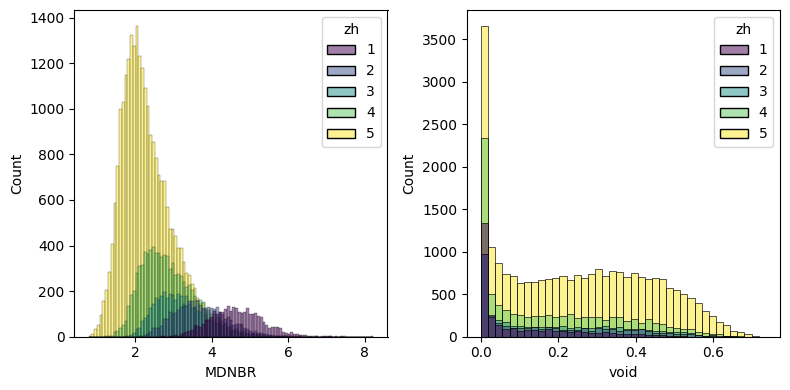
\includegraphics[width=\textwidth]{Figures/hist_void_mdnbr.png}
    \caption{Histogramas de fracción de vacío y MDNBR para las simulaciones con COBRA3-CP.}
    \label{fig:hist_void_mdnbr}
\end{figure}

Al realizar las simulaciones y procesarlas se generó un archivo con extensión \texttt{csv}, que tiene las siguientes columnas: \texttt{caso}, \texttt{canal}, \texttt{zh}, \texttt{pa1}, \texttt{...}, \texttt{pa22}, \texttt{pr1}, \texttt{...}, \texttt{pr37}, \texttt{power}, \texttt{void}, \texttt{caudal}, \texttt{temperatura}, \texttt{presion}, \texttt{MDNBR}. Este archivo fue importado como un objeto \texttt{pandas.DataFrame}, de la biblioteca pandas.

Se filtraron los resultados a utilizar por el valor de MDNBR y fracción de vacío, para utilizar sólo valores en el rango de interés al calcular las PLC. Los datos por fuera de estos rangos sirven de set adicional de evaluación, para determinar la capacidad de generalización del modelo por fuera del rango entrenado. Se filtraron los casos con MDNBR entre 1,7 y 2,5, o fracción de vacío entre 15\% y 35\%.

Con los resultados filtrados el pipeline es el siguiente:
\begin{enumerate}
    \item Conversión a tensores (\texttt{torch.tensor(, dtype=torch.float32)}) para las \textit{features} (todas las variables menos \texttt{MDNBR} y \texttt{void}) y \textit{target}.
    \item División entre \textit{train} y \textit{test} por medio de \texttt{train\_test\_split} de scikit-learn.
    \item Normalización de tensores de \textit{features} y \textit{targets} por medio de la función \texttt{plc.scale\_tensors()}, que utiliza por dentro \texttt{StandardScaler()} de scikit-learn.
\end{enumerate}

\subsection{Arquitectura del modelo, entrenamiento y optimización}
El estimador de PLC utiliza una arquitectura estándar de DNN, a partir del módulo \texttt{torch.nn.Sequential} y su método \texttt{add\_module()}. Los hiperparámetros a configurar son: cantidad de capas ocultas, cantidad de neuronas en las capas ocultas, función de activación, \textit{learning rate}, y tamaño del \textit{batch} de entrenamiento. 

En la figura \ref{fig:mlp-arquitectura} se esquematiza la arquitectura implementada. La entrada reúne las 63 variables mencionadas previamente: 22 componentes del perfil axial, las 37 componentes del perfil radial, y las condiciones de operación: potencia, caudal, temperatura y presión. A estas se aplica en la capa de entrada una función de activación $\sigma$. A continuación, estas variables ingresan en una red de \texttt{L} capas ocultas con \texttt{h} neuronas cada una, que aplican $\sigma$ en cada nodo. Por último la capa de salida tiene 2 variables: MDNBR y fracción de vacío.

% Arquitectura del perceptron multicapa (MLP).
%
% Fragmento para % Arquitectura del perceptron multicapa (MLP).
%
% Fragmento para \input{Figures/mlp_arquitectura}.
% Requiere en el preambulo del documento principal:
%   \usepackage{tikz}
%   \usetikzlibrary{decorations.pathreplacing}
%   \usepackage{amsmath,amssymb}
%
% Entradas (63): pa_1..pa_22, pr_1..pr_37, power, caudal, temperatura, presion.
% Salidas (2):   MDNBR, void.
% h = hidden_dim, L = cantidad de bloques lineal+activacion repetidos,
% sigma = funcion de activacion.
% La red tiene L+1 capas ocultas: la primera proviene de la capa lineal de
% entrada y las L restantes del bloque repetido.

\begin{figure}[htbp]
  \centering
  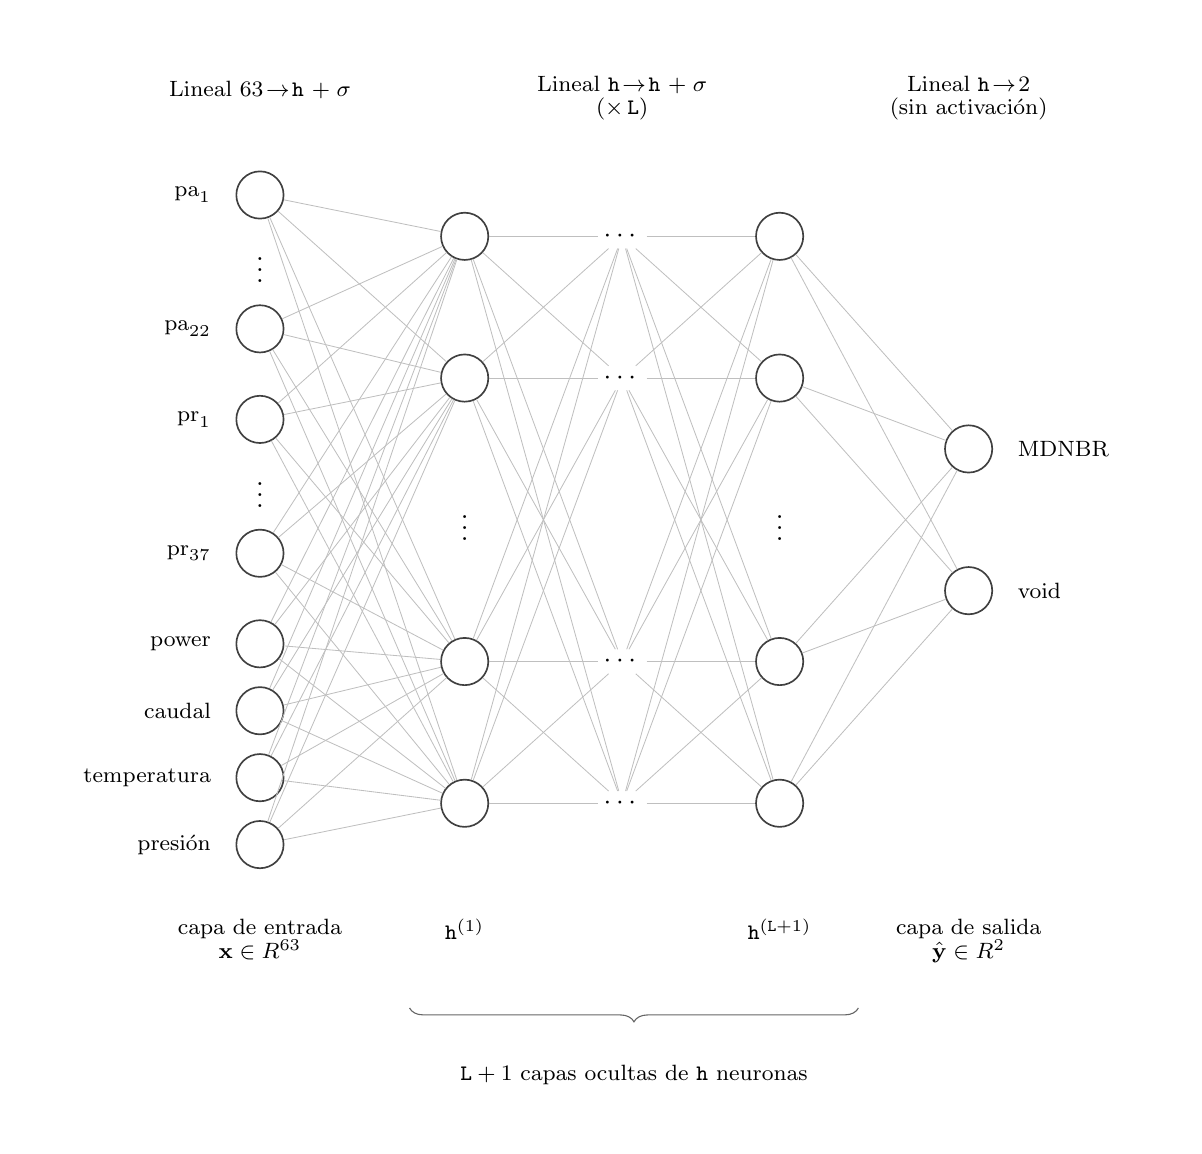
\begin{tikzpicture}[
      neurona/.style  = {circle, draw=black!75, fill=white, line width=0.6pt,
                         minimum size=6mm, inner sep=0pt},
      conexion/.style = {draw=black!25, line width=0.3pt},
      puntos/.style   = {inner sep=2pt},
      nombre/.style   = {font=\footnotesize},
      texto/.style    = {font=\footnotesize, align=center},
    ]
    \useasboundingbox (-2.95,-7.7) rectangle (11.6,6.25);

    %------------------------------------------------ capa de entrada (63)
    \foreach \y/\etq [count=\i] in {%
        4.125/$\mathrm{pa}_{1}$,
        2.425/$\mathrm{pa}_{22}$,
        1.275/$\mathrm{pr}_{1}$,
        -0.425/$\mathrm{pr}_{37}$,
        -1.575/power,
        -2.425/caudal,
        -3.275/temperatura,
        -4.125/presi\'on} {
      \node[neurona] (I-\i) at (0,\y) {};
      \node[nombre, anchor=east] at (-0.5,\y) {\etq};
    }
    \node[puntos] at (0,3.275) {$\vdots$};
    \node[puntos] at (0,0.425) {$\vdots$};

    %------------------------------------------------ primera capa oculta
    \foreach \y [count=\i] in {3.6, 1.8, -1.8, -3.6}
      \node[neurona] (H-\i) at (2.6,\y) {};
    \node[puntos] at (2.6,0) {$\vdots$};

    %------------------------------------------------ capas ocultas elididas
    \foreach \y [count=\i] in {3.6, 1.8, -1.8, -3.6}
      \node[puntos] (D-\i) at (4.6,\y) {$\cdots$};

    %------------------------------------------------ ultima capa oculta
    \foreach \y [count=\i] in {3.6, 1.8, -1.8, -3.6}
      \node[neurona] (G-\i) at (6.6,\y) {};
    \node[puntos] at (6.6,0) {$\vdots$};

    %------------------------------------------------ capa de salida (2)
    \foreach \y/\etq [count=\i] in {0.9/MDNBR, -0.9/void} {
      \node[neurona] (O-\i) at (9.0,\y) {};
      \node[nombre, anchor=west] at (9.5,\y) {\etq};
    }

    %------------------------------------------------ conexiones densas
    \foreach \a in {1,...,8}
      \foreach \b in {1,...,4}
        \draw[conexion] (I-\a) -- (H-\b);
    \foreach \a in {1,...,4}
      \foreach \b in {1,...,4} {
        \draw[conexion] (H-\a) -- (D-\b);
        \draw[conexion] (D-\a) -- (G-\b);
      }
    \foreach \a in {1,...,4}
      \foreach \b in {1,2}
        \draw[conexion] (G-\a) -- (O-\b);

    %------------------------------------------------ transformaciones
    \node[texto, anchor=south] at (0,4.95)
      {Lineal $63\!\to\!\texttt{h}$ $+\;\sigma$\\[-1pt]};
    \node[texto, anchor=south] at (4.6,4.95)
      {Lineal $\texttt{h}\!\to\!\texttt{h}$ $+\;\sigma$\\[-1pt] ($\times\,\texttt{L}$)};
    \node[texto, anchor=south] at (9,4.95)
      {Lineal $\texttt{h}\!\to\!2$\\[-1pt] (sin activaci\'on)};

    %------------------------------------------------ nombres de las capas
    \node[texto, anchor=north] at (0,-4.95)
      {capa de entrada\\[-1pt] $\mathbf{x}\in\mathbb{R}^{63}$};
    \node[texto, anchor=north] at (2.6,-4.95) {$\mathbf{\texttt{h}}^{(1)}$};
    \node[texto, anchor=north] at (6.6,-4.95) {$\mathbf{\texttt{h}}^{(\texttt{L}+1)}$};
    \node[texto, anchor=north] at (9.0,-4.95)
      {capa de salida\\[-1pt] $\hat{\mathbf{y}}\in\mathbb{R}^{2}$};

    %------------------------------------------------ llave de capas ocultas
    \draw[decorate, decoration={brace, amplitude=5pt, mirror}, draw=black!60]
      (1.9,-6.2) -- (7.6,-6.2);
    \node[texto, anchor=north] at (4.75,-6.8)
      {$\texttt{L}+1$ capas ocultas de \texttt{h} neuronas};
  \end{tikzpicture}
  \caption{Arquitectura de la DNN para estimación de MDNBR y fracción de vacío, para predicción de PLC.}
  \label{fig:mlp-arquitectura}
\end{figure}
.
% Requiere en el preambulo del documento principal:
%   \usepackage{tikz}
%   \usetikzlibrary{decorations.pathreplacing}
%   \usepackage{amsmath,amssymb}
%
% Entradas (63): pa_1..pa_22, pr_1..pr_37, power, caudal, temperatura, presion.
% Salidas (2):   MDNBR, void.
% h = hidden_dim, L = cantidad de bloques lineal+activacion repetidos,
% sigma = funcion de activacion.
% La red tiene L+1 capas ocultas: la primera proviene de la capa lineal de
% entrada y las L restantes del bloque repetido.

\begin{figure}[htbp]
  \centering
  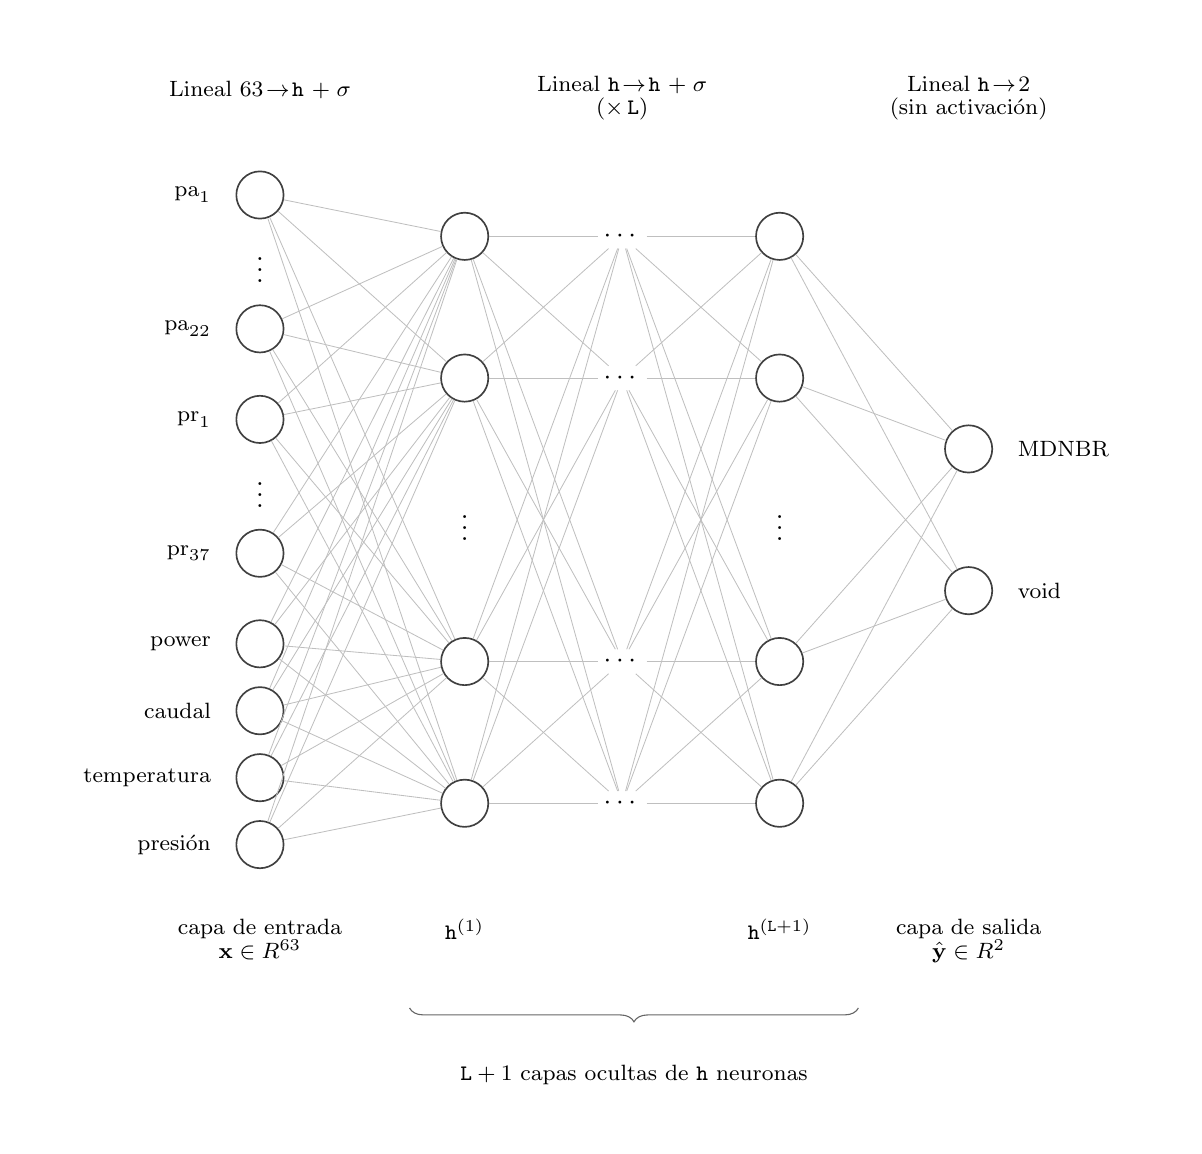
\begin{tikzpicture}[
      neurona/.style  = {circle, draw=black!75, fill=white, line width=0.6pt,
                         minimum size=6mm, inner sep=0pt},
      conexion/.style = {draw=black!25, line width=0.3pt},
      puntos/.style   = {inner sep=2pt},
      nombre/.style   = {font=\footnotesize},
      texto/.style    = {font=\footnotesize, align=center},
    ]
    \useasboundingbox (-2.95,-7.7) rectangle (11.6,6.25);

    %------------------------------------------------ capa de entrada (63)
    \foreach \y/\etq [count=\i] in {%
        4.125/$\mathrm{pa}_{1}$,
        2.425/$\mathrm{pa}_{22}$,
        1.275/$\mathrm{pr}_{1}$,
        -0.425/$\mathrm{pr}_{37}$,
        -1.575/power,
        -2.425/caudal,
        -3.275/temperatura,
        -4.125/presi\'on} {
      \node[neurona] (I-\i) at (0,\y) {};
      \node[nombre, anchor=east] at (-0.5,\y) {\etq};
    }
    \node[puntos] at (0,3.275) {$\vdots$};
    \node[puntos] at (0,0.425) {$\vdots$};

    %------------------------------------------------ primera capa oculta
    \foreach \y [count=\i] in {3.6, 1.8, -1.8, -3.6}
      \node[neurona] (H-\i) at (2.6,\y) {};
    \node[puntos] at (2.6,0) {$\vdots$};

    %------------------------------------------------ capas ocultas elididas
    \foreach \y [count=\i] in {3.6, 1.8, -1.8, -3.6}
      \node[puntos] (D-\i) at (4.6,\y) {$\cdots$};

    %------------------------------------------------ ultima capa oculta
    \foreach \y [count=\i] in {3.6, 1.8, -1.8, -3.6}
      \node[neurona] (G-\i) at (6.6,\y) {};
    \node[puntos] at (6.6,0) {$\vdots$};

    %------------------------------------------------ capa de salida (2)
    \foreach \y/\etq [count=\i] in {0.9/MDNBR, -0.9/void} {
      \node[neurona] (O-\i) at (9.0,\y) {};
      \node[nombre, anchor=west] at (9.5,\y) {\etq};
    }

    %------------------------------------------------ conexiones densas
    \foreach \a in {1,...,8}
      \foreach \b in {1,...,4}
        \draw[conexion] (I-\a) -- (H-\b);
    \foreach \a in {1,...,4}
      \foreach \b in {1,...,4} {
        \draw[conexion] (H-\a) -- (D-\b);
        \draw[conexion] (D-\a) -- (G-\b);
      }
    \foreach \a in {1,...,4}
      \foreach \b in {1,2}
        \draw[conexion] (G-\a) -- (O-\b);

    %------------------------------------------------ transformaciones
    \node[texto, anchor=south] at (0,4.95)
      {Lineal $63\!\to\!\texttt{h}$ $+\;\sigma$\\[-1pt]};
    \node[texto, anchor=south] at (4.6,4.95)
      {Lineal $\texttt{h}\!\to\!\texttt{h}$ $+\;\sigma$\\[-1pt] ($\times\,\texttt{L}$)};
    \node[texto, anchor=south] at (9,4.95)
      {Lineal $\texttt{h}\!\to\!2$\\[-1pt] (sin activaci\'on)};

    %------------------------------------------------ nombres de las capas
    \node[texto, anchor=north] at (0,-4.95)
      {capa de entrada\\[-1pt] $\mathbf{x}\in\mathbb{R}^{63}$};
    \node[texto, anchor=north] at (2.6,-4.95) {$\mathbf{\texttt{h}}^{(1)}$};
    \node[texto, anchor=north] at (6.6,-4.95) {$\mathbf{\texttt{h}}^{(\texttt{L}+1)}$};
    \node[texto, anchor=north] at (9.0,-4.95)
      {capa de salida\\[-1pt] $\hat{\mathbf{y}}\in\mathbb{R}^{2}$};

    %------------------------------------------------ llave de capas ocultas
    \draw[decorate, decoration={brace, amplitude=5pt, mirror}, draw=black!60]
      (1.9,-6.2) -- (7.6,-6.2);
    \node[texto, anchor=north] at (4.75,-6.8)
      {$\texttt{L}+1$ capas ocultas de \texttt{h} neuronas};
  \end{tikzpicture}
  \caption{Arquitectura de la DNN para estimación de MDNBR y fracción de vacío, para predicción de PLC.}
  \label{fig:mlp-arquitectura}
\end{figure}


Para el armado de la arquitectura se desarrolló la función \texttt{plc.build\_model} que permite en una línea obtener el modelo con los hiperparámetros deseados.

Para entrenar al modelo se utilizó Adam \citep{kingma2015adam} como optimizador, debido a su alta capacidad y adopción en casos clásicos de DNN. Como función de pérdida se utilizó la raíz del error cuadrático medio (RMSE, del inglés \textit{Root Mean Squared Error}), debido a que penaliza fuertemente los errores grandes y tiene magnitud del orden de las variables a optimizar.

Durante el entrenamiento se evalúa, además de la función de pérdida, el coeficiente de correlación $\text{R}^2$, tanto para el set de entrenamiento como el de evaluación. Al predecir sobre el set de evaluación, se utiliza la condición \texttt{torch.no\_grad()} para evitar que se aprenda de este set de datos y genere \textit{data leakage}. Se desarrolló la función de ayuda \texttt{plc.train\_model} para realizar el entrenamiento sobre la cantidad de épocas deseadas de forma sencilla.

La definición de los hiperparámetros se realiza por medio de su optimización con optuna. Para ello se plantea un estudio de hiperparámetros con 50 \textit{trials} de 200 épocas cada uno. Se consideraron DNN con entre 2 y 15 capas ocultas, de entre 32 y 512 neuronas cada uno, con un \textit{learning rate} de entre $10^{-2}$ y $10^{-5}$ y \textit{batches} de entrenamiento de entre 16 y 236.
Las funciones de activación consideradas fueron: ReLU \citep{nair2010rectified}, GELU \citep{hendrycks2016gaussian}, SiLU/Swish \citep{elfwing2018sigmoid}, Tanh, Leaky ReLU \citep{maas2013rectifier} y ELU \citep{clevert2015fast}.

En el capítulo \ref{Chapter4} se presentan los resultados de la optimización realizada.

\subsection{Integración e implementación del sistema}
La integración consiste en realizar el lazo de cálculo de PLC de COBRA, pero con la DNN entrenada en su lugar. Se tiene un lazo para cada límite de PLC, pero son idénticos en concepto. Únicamente se debe modificar la variable objetivo según si es criterio de DNB o de fracción de vacío.

El lazo de cálculo se esquematiza en la figura \ref{fig:dnb-dnn-loop}. En la misma se observa que en primer lugar se deben definir las condiciones operativas, esto es, temperatura y presión, y el límite objetivo, ya sea de MDNBR o de fracción de vacío. Luego se realizan dos cálculos, uno de piso y otro de techo, donde se evalúan los flujos de calor mínimo y máximo. Estos valores se establecen de antemano y se deben proveer valores que contengan al flujo de calor correspondiente al límite objetivo, por lo que un rango amplio es recomendable. Se obtiene el valor del límite para el flujo de calor mínimo y máximo, y por el método de la secante se estima el flujo de calor que debería obtener el límite objetivo. Se recalcula el caudal másico con dicho flujo de calor, y se vuelve a estimar el límite. Si se obtiene convergencia tanto en el límite objetivo, como en caudal y flujo de calor, se termina el lazo de cálculo. Si no se obtiene convergencia, se realiza una nueva iteración del método de la secante.

Para calcular el flujo másico en función del flujo de calor, se recurre a la relación caudal-potencia desarrollada por INVAP en \citep{invap_caudal_potencia}, donde para cada ZH y condición operativa se tiene una tabla para interpolar caudal másico a partir de potencia de canal.

% Lazo de calculo del flujo de calor que alcanza el MDNBR objetivo.
%
% Fragmento para % Lazo de calculo del flujo de calor que alcanza el MDNBR objetivo.
%
% Fragmento para \input{Figures/dnb_dnn_loop}.
% Requiere en el preambulo del documento principal:
%   \usepackage{tikz}
%   \usetikzlibrary{arrows.meta}
%   \usepackage{amsmath,amssymb}
%
% Estructura: condiciones de operacion -> ramas paralelas de piso (q''_min) y
% techo (q''_max), cada una con establecer flujo, calcular caudal masico y
% predecir MDNBR con la DNN -> lazo de la secante, con el calculo del caudal
% masico y la prediccion de la DNN como pasos separados, hasta cumplir el
% criterio de convergencia.
%
% Los tres pasos que invocan a la red llevan un esquema en miniatura de la DNN
% (pic "dnnmini"), consistente con fig:mlp-arquitectura.

\begin{figure}[htbp]
  \centering
  \resizebox{\textwidth}{!}{
  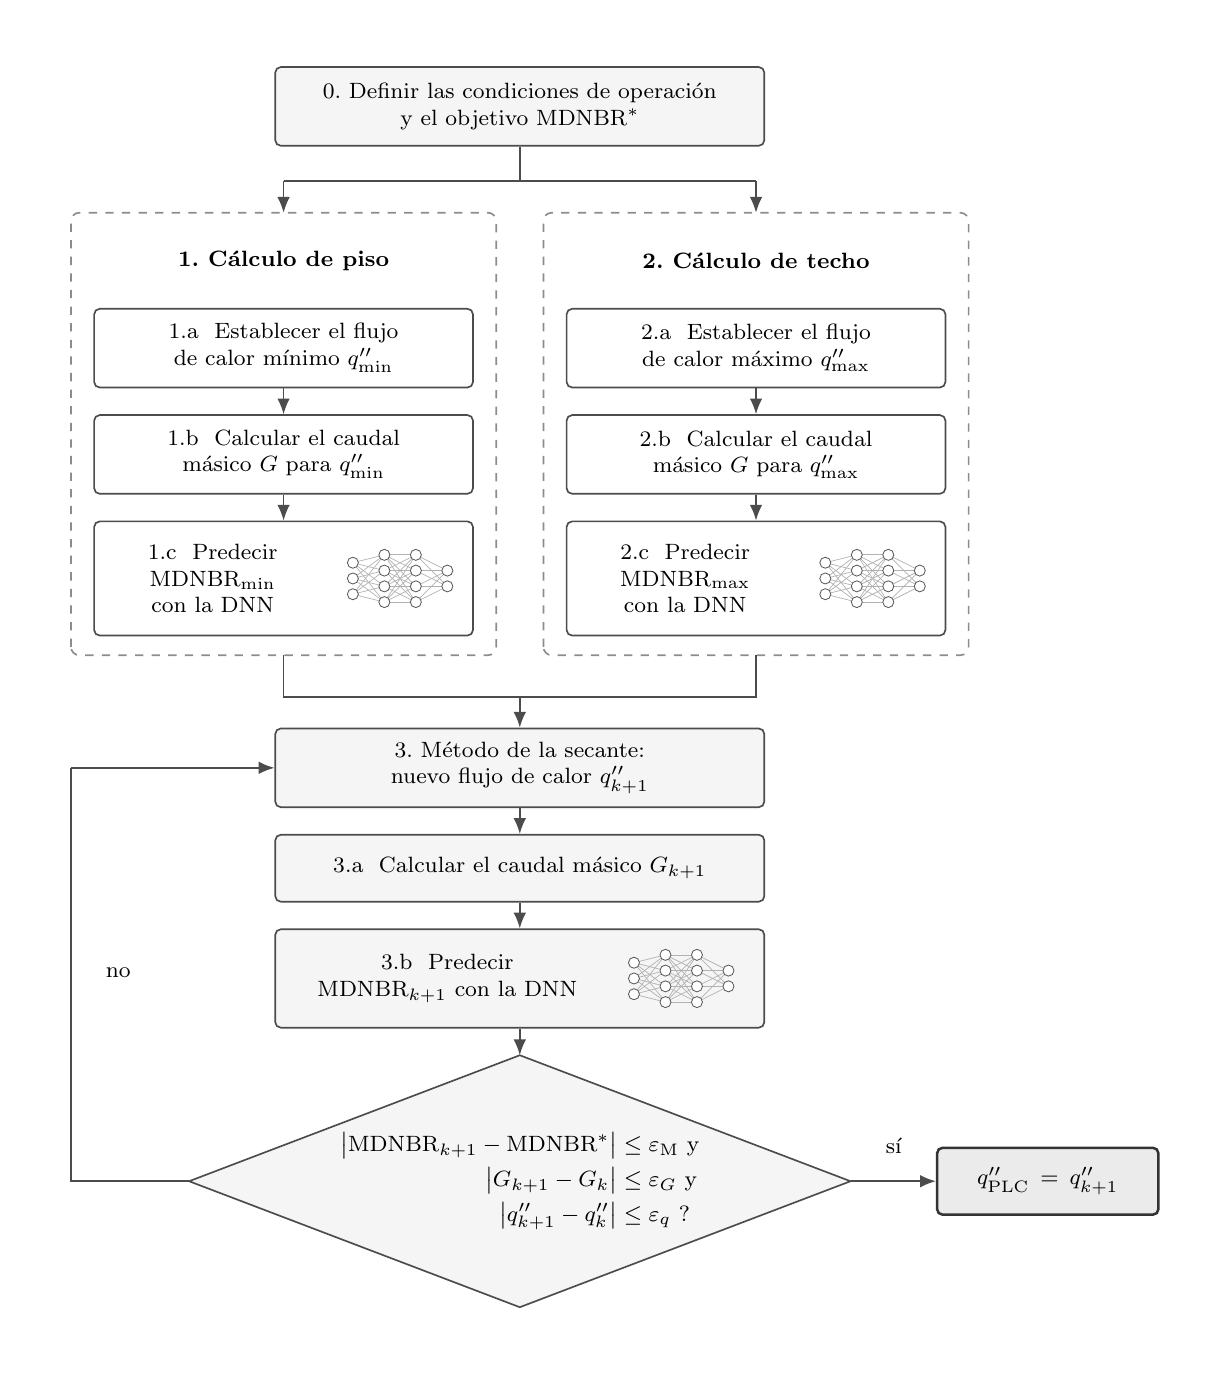
\begin{tikzpicture}[
      caja/.style   = {rectangle, rounded corners=2pt, draw=black!70,
                       fill=black!4, line width=0.6pt, text width=6.0cm,
                       align=center, font=\footnotesize, minimum height=1.0cm,
                       inner sep=3pt},
      subcaja/.style= {rectangle, rounded corners=2pt, draw=black!70,
                       fill=white, line width=0.6pt, text width=4.6cm,
                       align=center, font=\footnotesize, minimum height=1.0cm,
                       inner sep=3pt},
      final/.style  = {rectangle, rounded corners=2pt, draw=black!80,
                       fill=black!8, line width=0.9pt, text width=2.6cm,
                       align=center, font=\footnotesize, minimum height=0.85cm,
                       inner sep=3pt},
      grupo/.style  = {rectangle, rounded corners=3pt, draw=black!45,
                       line width=0.6pt, dashed},
      titulo/.style = {font=\footnotesize\bfseries, inner sep=1pt},
      rombo/.style  = {draw=black!70, fill=black!4, line width=0.6pt},
      texto/.style  = {font=\footnotesize, align=center, inner sep=1pt},
      nombre/.style = {font=\footnotesize, inner sep=1pt},
      flecha/.style = {-{Latex[length=2mm,width=1.6mm]}, draw=black!70,
                       line width=0.6pt},
      linea/.style  = {draw=black!70, line width=0.6pt},
      %--- estilos del esquema en miniatura de la red
      nnnodo/.style = {circle, draw=black!65, fill=white, line width=0.3pt,
                       minimum size=1.4mm, inner sep=0pt},
      nnarco/.style = {draw=black!30, line width=0.25pt},
      %--- esquema en miniatura de la DNN (3 entradas, 4+4 ocultas, 2 salidas)
      dnnmini/.pic  = {
        \foreach \ya in {0.20,0,-0.20}
          \foreach \yb in {0.30,0.10,-0.10,-0.30}
            \draw[nnarco] (0,\ya) -- (0.4,\yb);
        \foreach \ya in {0.30,0.10,-0.10,-0.30}
          \foreach \yb in {0.30,0.10,-0.10,-0.30}
            \draw[nnarco] (0.4,\ya) -- (0.8,\yb);
        \foreach \ya in {0.30,0.10,-0.10,-0.30}
          \foreach \yb in {0.10,-0.10}
            \draw[nnarco] (0.8,\ya) -- (1.2,\yb);
        \foreach \y in {0.20,0,-0.20}
          \node[nnnodo] at (0,\y) {};
        \foreach \y in {0.30,0.10,-0.10,-0.30} {
          \node[nnnodo] at (0.4,\y) {};
          \node[nnnodo] at (0.8,\y) {};
        }
        \foreach \y in {0.10,-0.10}
          \node[nnnodo] at (1.2,\y) {};
      },
    ]
    \useasboundingbox (-6.25,-15.80) rectangle (8.61,1.0);

    %-------------------------------------------------- 0. condiciones
    \node[caja] (A) at (0,0)
      {0.~Definir las condiciones de operaci\'on\\
       y el objetivo $\mathrm{MDNBR}^{*}$};

    %-------------------------------------------------- marcos de las ramas
    \draw[grupo] (-5.7,-6.97) rectangle (-0.3,-1.35);
    \draw[grupo] ( 0.3,-6.97) rectangle ( 5.7,-1.35);

    \node[titulo] at (-3.0,-1.96) {1.~C\'alculo de piso};
    \node[titulo] at ( 3.0,-1.96) {2.~C\'alculo de techo};

    %-------------------------------------------------- rama de piso
    \node[subcaja] (P1) at (-3.0,-3.07)
      {1.a~~Establecer el flujo\\ de calor m\'inimo $q''_{\min}$};
    \node[subcaja] (P2) at (-3.0,-4.42)
      {1.b~~Calcular el caudal\\ m\'asico $G$ para $q''_{\min}$};
    \node[subcaja, minimum height=1.45cm] (P3) at (-3.0,-5.995) {};
    \node[texto, text width=2.5cm] at (-3.90,-5.995)
      {1.c~~Predecir $\mathrm{MDNBR}_{\min}$ con la DNN};
    \pic at (-2.12,-5.995) {dnnmini};

    %-------------------------------------------------- rama de techo
    \node[subcaja] (T1) at (3.0,-3.07)
      {2.a~~Establecer el flujo\\ de calor m\'aximo $q''_{\max}$};
    \node[subcaja] (T2) at (3.0,-4.42)
      {2.b~~Calcular el caudal\\ m\'asico $G$ para $q''_{\max}$};
    \node[subcaja, minimum height=1.45cm] (T3) at (3.0,-5.995) {};
    \node[texto, text width=2.5cm] at (2.10,-5.995)
      {2.c~~Predecir $\mathrm{MDNBR}_{\max}$ con la DNN};
    \pic at (3.88,-5.995) {dnnmini};

    %-------------------------------------------------- lazo de la secante
    \node[caja] (C) at (0,-8.40)
      {3.~M\'etodo de la secante:\\
       nuevo flujo de calor $q''_{k+1}$};

    \node[caja, minimum height=0.85cm] (D1) at (0,-9.675)
      {3.a~~Calcular el caudal m\'asico $G_{k+1}$};

    \node[caja, minimum height=1.25cm] (D2) at (0,-11.075) {};
    \node[texto, text width=3.6cm] at (-0.92,-11.075)
      {3.b~~Predecir $\mathrm{MDNBR}_{k+1}$ con la DNN};
    \pic at (1.45,-11.075) {dnnmini};

    %-------------------------------------------------- criterio de convergencia
    \draw[rombo] (0,-12.05) -- (4.2,-13.65) -- (0,-15.25) -- (-4.2,-13.65)
      -- cycle;
    \node[texto] at (0,-13.65)
      {$\begin{aligned}
         \bigl|\mathrm{MDNBR}_{k+1}-\mathrm{MDNBR}^{*}\bigr|
           &\le\varepsilon_{\mathrm{M}} \ \text{y} \\[-1pt]
         \bigl|G_{k+1}-G_{k}\bigr| &\le\varepsilon_{G} \ \text{y} \\[-1pt]
         \bigl|q''_{k+1}-q''_{k}\bigr| &\le\varepsilon_{q} \ ?
       \end{aligned}$};

    \node[final] (F) at (6.705,-13.65) {$q''_{\mathrm{PLC}}=q''_{k+1}$};

    %-------------------------------------------------- flujo: 0 -> ramas
    \draw[linea]  (A.south) -- (0,-0.95);
    \draw[linea]  (-3.0,-0.95) -- (3.0,-0.95);
    \draw[flecha] (-3.0,-0.95) -- (-3.0,-1.35);
    \draw[flecha] ( 3.0,-0.95) -- ( 3.0,-1.35);

    %-------------------------------------------------- flujo dentro de cada rama
    \draw[flecha] (P1.south) -- (P2.north);
    \draw[flecha] (P2.south) -- (P3.north);
    \draw[flecha] (T1.south) -- (T2.north);
    \draw[flecha] (T2.south) -- (T3.north);

    %-------------------------------------------------- ramas -> secante
    \draw[linea]  (-3.0,-6.97) -- (-3.0,-7.50) -- (0,-7.50);
    \draw[linea]  ( 3.0,-6.97) -- ( 3.0,-7.50) -- (0,-7.50);
    \draw[flecha] (0,-7.50) -- (C.north);

    %-------------------------------------------------- lazo
    \draw[flecha] (C.south)  -- (D1.north);
    \draw[flecha] (D1.south) -- (D2.north);
    \draw[flecha] (D2.south) -- (0,-12.05);

    \draw[flecha] (4.2,-13.65) -- (F.west);
    \node[nombre] at (4.75,-13.20) {s\'i};

    \draw[linea]  (-4.2,-13.65) -- (-5.7,-13.65) -- (-5.7,-8.40);
    \draw[flecha] (-5.7,-8.40) -- (C.west);
    \node[nombre, anchor=west] at (-5.3,-11.0) {no};
  \end{tikzpicture}}
  \caption{Lazo de c\'alculo del flujo de calor que alcanza el MDNBR objetivo.}
  \label{fig:dnb-dnn-loop}
\end{figure}
.
% Requiere en el preambulo del documento principal:
%   \usepackage{tikz}
%   \usetikzlibrary{arrows.meta}
%   \usepackage{amsmath,amssymb}
%
% Estructura: condiciones de operacion -> ramas paralelas de piso (q''_min) y
% techo (q''_max), cada una con establecer flujo, calcular caudal masico y
% predecir MDNBR con la DNN -> lazo de la secante, con el calculo del caudal
% masico y la prediccion de la DNN como pasos separados, hasta cumplir el
% criterio de convergencia.
%
% Los tres pasos que invocan a la red llevan un esquema en miniatura de la DNN
% (pic "dnnmini"), consistente con fig:mlp-arquitectura.

\begin{figure}[htbp]
  \centering
  \resizebox{\textwidth}{!}{
  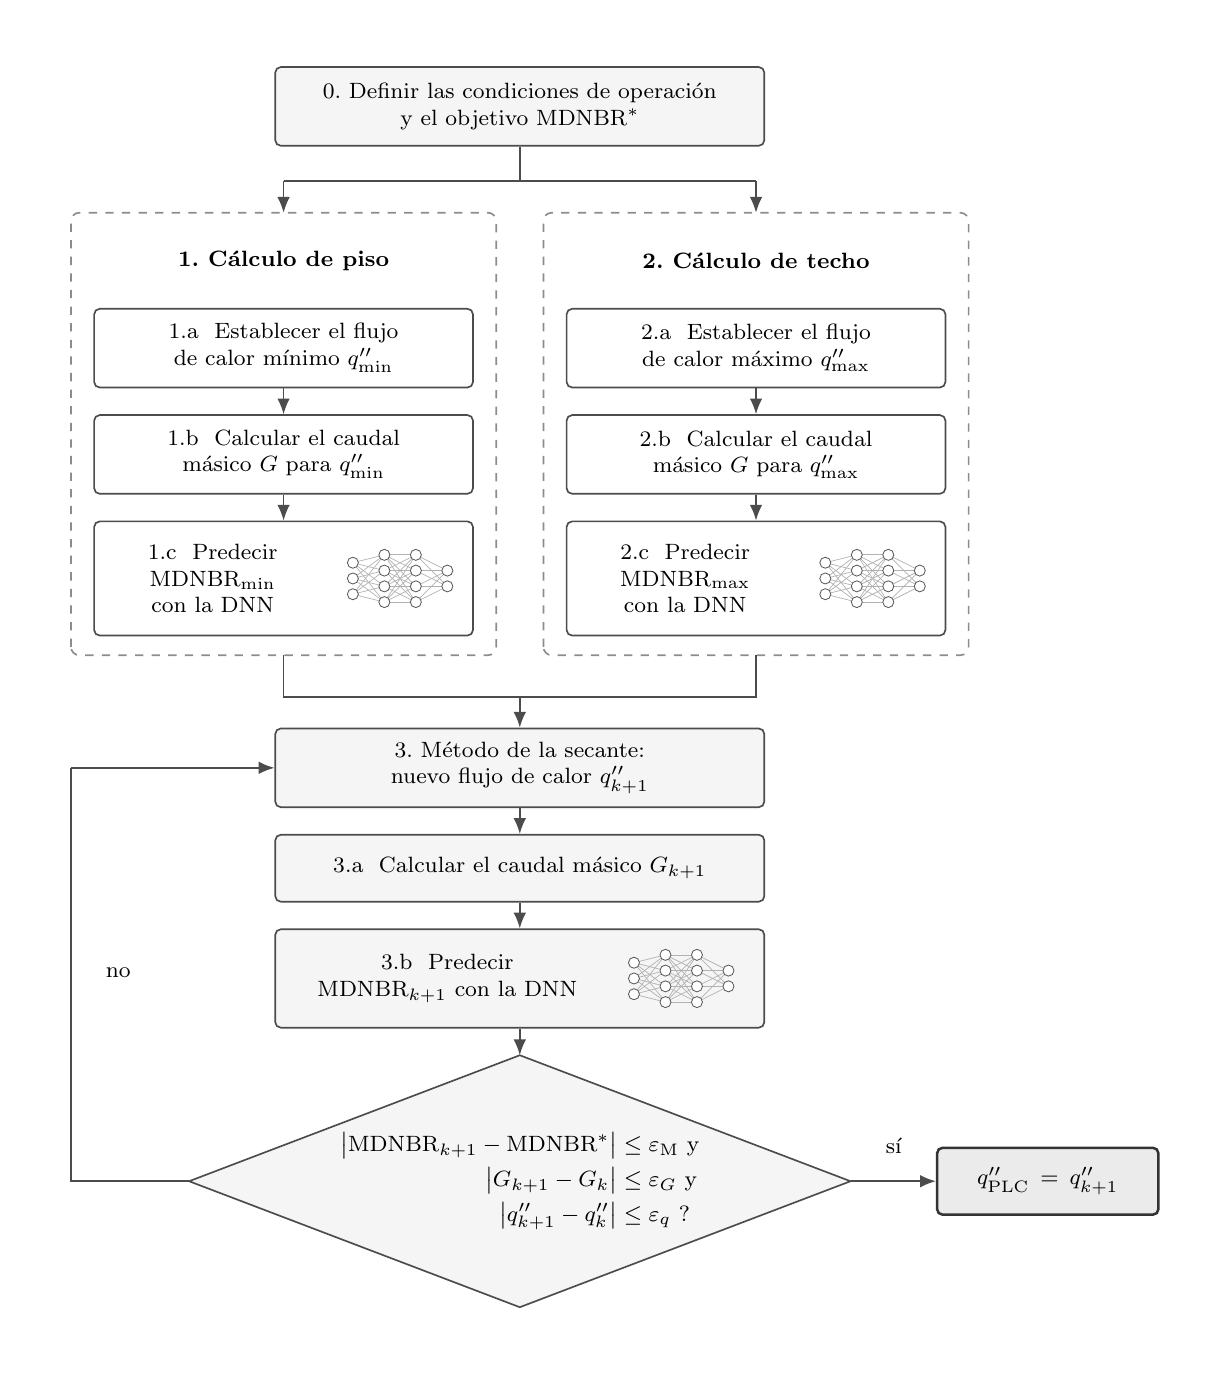
\begin{tikzpicture}[
      caja/.style   = {rectangle, rounded corners=2pt, draw=black!70,
                       fill=black!4, line width=0.6pt, text width=6.0cm,
                       align=center, font=\footnotesize, minimum height=1.0cm,
                       inner sep=3pt},
      subcaja/.style= {rectangle, rounded corners=2pt, draw=black!70,
                       fill=white, line width=0.6pt, text width=4.6cm,
                       align=center, font=\footnotesize, minimum height=1.0cm,
                       inner sep=3pt},
      final/.style  = {rectangle, rounded corners=2pt, draw=black!80,
                       fill=black!8, line width=0.9pt, text width=2.6cm,
                       align=center, font=\footnotesize, minimum height=0.85cm,
                       inner sep=3pt},
      grupo/.style  = {rectangle, rounded corners=3pt, draw=black!45,
                       line width=0.6pt, dashed},
      titulo/.style = {font=\footnotesize\bfseries, inner sep=1pt},
      rombo/.style  = {draw=black!70, fill=black!4, line width=0.6pt},
      texto/.style  = {font=\footnotesize, align=center, inner sep=1pt},
      nombre/.style = {font=\footnotesize, inner sep=1pt},
      flecha/.style = {-{Latex[length=2mm,width=1.6mm]}, draw=black!70,
                       line width=0.6pt},
      linea/.style  = {draw=black!70, line width=0.6pt},
      %--- estilos del esquema en miniatura de la red
      nnnodo/.style = {circle, draw=black!65, fill=white, line width=0.3pt,
                       minimum size=1.4mm, inner sep=0pt},
      nnarco/.style = {draw=black!30, line width=0.25pt},
      %--- esquema en miniatura de la DNN (3 entradas, 4+4 ocultas, 2 salidas)
      dnnmini/.pic  = {
        \foreach \ya in {0.20,0,-0.20}
          \foreach \yb in {0.30,0.10,-0.10,-0.30}
            \draw[nnarco] (0,\ya) -- (0.4,\yb);
        \foreach \ya in {0.30,0.10,-0.10,-0.30}
          \foreach \yb in {0.30,0.10,-0.10,-0.30}
            \draw[nnarco] (0.4,\ya) -- (0.8,\yb);
        \foreach \ya in {0.30,0.10,-0.10,-0.30}
          \foreach \yb in {0.10,-0.10}
            \draw[nnarco] (0.8,\ya) -- (1.2,\yb);
        \foreach \y in {0.20,0,-0.20}
          \node[nnnodo] at (0,\y) {};
        \foreach \y in {0.30,0.10,-0.10,-0.30} {
          \node[nnnodo] at (0.4,\y) {};
          \node[nnnodo] at (0.8,\y) {};
        }
        \foreach \y in {0.10,-0.10}
          \node[nnnodo] at (1.2,\y) {};
      },
    ]
    \useasboundingbox (-6.25,-15.80) rectangle (8.61,1.0);

    %-------------------------------------------------- 0. condiciones
    \node[caja] (A) at (0,0)
      {0.~Definir las condiciones de operaci\'on\\
       y el objetivo $\mathrm{MDNBR}^{*}$};

    %-------------------------------------------------- marcos de las ramas
    \draw[grupo] (-5.7,-6.97) rectangle (-0.3,-1.35);
    \draw[grupo] ( 0.3,-6.97) rectangle ( 5.7,-1.35);

    \node[titulo] at (-3.0,-1.96) {1.~C\'alculo de piso};
    \node[titulo] at ( 3.0,-1.96) {2.~C\'alculo de techo};

    %-------------------------------------------------- rama de piso
    \node[subcaja] (P1) at (-3.0,-3.07)
      {1.a~~Establecer el flujo\\ de calor m\'inimo $q''_{\min}$};
    \node[subcaja] (P2) at (-3.0,-4.42)
      {1.b~~Calcular el caudal\\ m\'asico $G$ para $q''_{\min}$};
    \node[subcaja, minimum height=1.45cm] (P3) at (-3.0,-5.995) {};
    \node[texto, text width=2.5cm] at (-3.90,-5.995)
      {1.c~~Predecir $\mathrm{MDNBR}_{\min}$ con la DNN};
    \pic at (-2.12,-5.995) {dnnmini};

    %-------------------------------------------------- rama de techo
    \node[subcaja] (T1) at (3.0,-3.07)
      {2.a~~Establecer el flujo\\ de calor m\'aximo $q''_{\max}$};
    \node[subcaja] (T2) at (3.0,-4.42)
      {2.b~~Calcular el caudal\\ m\'asico $G$ para $q''_{\max}$};
    \node[subcaja, minimum height=1.45cm] (T3) at (3.0,-5.995) {};
    \node[texto, text width=2.5cm] at (2.10,-5.995)
      {2.c~~Predecir $\mathrm{MDNBR}_{\max}$ con la DNN};
    \pic at (3.88,-5.995) {dnnmini};

    %-------------------------------------------------- lazo de la secante
    \node[caja] (C) at (0,-8.40)
      {3.~M\'etodo de la secante:\\
       nuevo flujo de calor $q''_{k+1}$};

    \node[caja, minimum height=0.85cm] (D1) at (0,-9.675)
      {3.a~~Calcular el caudal m\'asico $G_{k+1}$};

    \node[caja, minimum height=1.25cm] (D2) at (0,-11.075) {};
    \node[texto, text width=3.6cm] at (-0.92,-11.075)
      {3.b~~Predecir $\mathrm{MDNBR}_{k+1}$ con la DNN};
    \pic at (1.45,-11.075) {dnnmini};

    %-------------------------------------------------- criterio de convergencia
    \draw[rombo] (0,-12.05) -- (4.2,-13.65) -- (0,-15.25) -- (-4.2,-13.65)
      -- cycle;
    \node[texto] at (0,-13.65)
      {$\begin{aligned}
         \bigl|\mathrm{MDNBR}_{k+1}-\mathrm{MDNBR}^{*}\bigr|
           &\le\varepsilon_{\mathrm{M}} \ \text{y} \\[-1pt]
         \bigl|G_{k+1}-G_{k}\bigr| &\le\varepsilon_{G} \ \text{y} \\[-1pt]
         \bigl|q''_{k+1}-q''_{k}\bigr| &\le\varepsilon_{q} \ ?
       \end{aligned}$};

    \node[final] (F) at (6.705,-13.65) {$q''_{\mathrm{PLC}}=q''_{k+1}$};

    %-------------------------------------------------- flujo: 0 -> ramas
    \draw[linea]  (A.south) -- (0,-0.95);
    \draw[linea]  (-3.0,-0.95) -- (3.0,-0.95);
    \draw[flecha] (-3.0,-0.95) -- (-3.0,-1.35);
    \draw[flecha] ( 3.0,-0.95) -- ( 3.0,-1.35);

    %-------------------------------------------------- flujo dentro de cada rama
    \draw[flecha] (P1.south) -- (P2.north);
    \draw[flecha] (P2.south) -- (P3.north);
    \draw[flecha] (T1.south) -- (T2.north);
    \draw[flecha] (T2.south) -- (T3.north);

    %-------------------------------------------------- ramas -> secante
    \draw[linea]  (-3.0,-6.97) -- (-3.0,-7.50) -- (0,-7.50);
    \draw[linea]  ( 3.0,-6.97) -- ( 3.0,-7.50) -- (0,-7.50);
    \draw[flecha] (0,-7.50) -- (C.north);

    %-------------------------------------------------- lazo
    \draw[flecha] (C.south)  -- (D1.north);
    \draw[flecha] (D1.south) -- (D2.north);
    \draw[flecha] (D2.south) -- (0,-12.05);

    \draw[flecha] (4.2,-13.65) -- (F.west);
    \node[nombre] at (4.75,-13.20) {s\'i};

    \draw[linea]  (-4.2,-13.65) -- (-5.7,-13.65) -- (-5.7,-8.40);
    \draw[flecha] (-5.7,-8.40) -- (C.west);
    \node[nombre, anchor=west] at (-5.3,-11.0) {no};
  \end{tikzpicture}}
  \caption{Lazo de c\'alculo del flujo de calor que alcanza el MDNBR objetivo.}
  \label{fig:dnb-dnn-loop}
\end{figure}


\subsection{Arquitectura de embeddings, entrenamiento y aplicación}


\pagebreak
\section{Estimación de CHF}
En esta sección se presenta el modelo de multifidelidad informado por física para estimar CHF. Se presenta el pipeline de datos, la arquitectura del modelo y la metodología para su evaluación.

Se desarrollaron múltiples códigos Python para ayudar con el desarrollo de las distintas tareas necesarias, a saber: \texttt{chf.py}, \texttt{ahmad\_scaling.py}, \texttt{softmin.py}, \texttt{import\_cobra.py}. 

\subsection{Pipeline de datos}
Los datos disponibles para estimación de CHF se dividen en tres fuentes:
\begin{itemize}
    \item Datos de ensayo en tubo, utilizados por Groeneveld para sus LUT (versión 2006).
    \item Datos de ensayos de la Universidad de Columbia, sobre el bundle de la CNA-UII.
    \item Datos de simulaciones de COBRA3-CP, que modelan la geometría y condiciones de los ensayos de la Universidad de Columbia.
\end{itemize}
Estas fuentes tienen distintas características. Los datos de ensayos experimentales tienen una disponibilidad similar de datos, aunque los ensayos de bundle conllevan una mayor complejidad geométrica, propia del bundle, que podría ser tenida en cuenta por el modelo. Es posible realizar \textit{data augmentation} de los datos experimentales por medio de modelos y relaciones termodinámicas. Por otro lado, las simulaciones permiten obtener datos muy detallados, tanto espacialmente como en variables termodinámicas informadas.

Por otro lado, se debe definir con cautela qué \textit{features} dar al modelo para predecir CHF. Si se considera que no hay pérdidas de calor, la evolución de la entalpía del fluido en función de la coordenada $z$ va a venir dada por:
\begin{equation}
    h(z) = h_\mathrm{inlet} + \frac{\pi\,D}{\dot{m}} \int_0^z q''\,dz'.
    \label{eq:hz}
\end{equation}
Por otro lado, el título termodinámico de equilibrio se relaciona con la entalpía de la siguiente forma:
\begin{equation}
    x(z) = \frac{h(z) - h_f}{h_{fg}}.
    \label{eq:xz}
\end{equation}
Si $q''=\mathrm{cte}$, como lo es tanto en los ensayos de un tubo y del bundle de la \cna{}, al reemplazar \ref{eq:hz} en \ref{eq:xz} se tiene:
\begin{equation}
    x(z) = x_\mathrm{inlet} + \frac{\pi\,D\,q''\,z}{\dot{m}\,h_{fg}},
\end{equation}
por lo que el modelo, dado $x(z=1)=x_\mathrm{outlet}$, puede despejar $q''$. Esto tiene dos implicancias: en primer lugar el modelo está asumiendo perfil de flujo de calor constante; y en segundo lugar, está considerando que las variables de entrada corresponden a un estado de CHF. Ninguna de estas dos implicancias son deseables, ya que el modelo no podrá generalizar a los casos de interés: cuando no se conoce el valor del CHF, ni se tiene un perfil de potencia uniforme.

En la bibliografía clásica de CHF existen dos enfoques: el método de sustitución directa (DSM, del inglés \textit{Direct Substitution Method}) y el método de balance de calor (HBM, del inglés \textit{Heat Balance Method}). El DSM tiene como principal hipótesis que el CHF es un fenómeno local, por lo que utiliza directamente variables locales para predecir CHF. Esta hipótesis se ha considerado relativamente válida en caso de DNB, como lo sugieren \citep{weisman1983, tong1997boiling, lecorre2010}. Por otro lado, el HBM, como lo indica su nombre, realiza el balance de calor a partir de las condiciones de entrada al tubo.
Groeneveld et al. evaluaron sus tres versiones de las LUT (1986 \citep{GROENEVELD1986}, 1995 y 2006) mediante ambos métodos, y obtuvieron predicciones más precisas mediante el HBM. 
Sin embargo, el DSM es el más utilizado en la práctica, y el más adecuado para su aplicación en códigos termohidráulicos, como señala Siman\=/Tov \citep{SIMANTOV1996}. Esto se debe, por un lado, a su simplicidad, y por otro, a que los ensayos realizados en geometrías reales (de bundle) informan las condiciones promedio, mientras que el CHF ocurre a nivel de subcanal. Las condiciones locales a nivel de subcanal pueden ser estimadas por medio de códigos de subcanal como COBRA3-CP, pero esto agregaría un error de la herramienta de cálculo que sería deseable evitar.
Adicionalmente, el DSM es el método utilizado en la estimación de CHF para el bundle de la \cna{}, por medio de las LUT 1995 y los TMF de INVAP.

% Entonces, en este trabajo, se analizarán dos \textit{pipelines} de datos, ambos basadas en DSM. En primer lugar considerar las mismas entradas que toma el método actual: \textcolor{red}{completar con lo que toma la LUT + lo que toman los factores de correccion de Groeneveld y los TMF de INVAP. Hay algunos datos que son específicos de la corrección de bundle.}. A este pipeline lo llamaremos \texttt{pipeline vanilla}.

% En segundo lugar, se realizará una transformación de las variables en números adimensionales, y se evaluará por medio de regularización y validación cruzada su relevancia. Las variables planteadas en este pipeline son: \textcolor{red}{completar!! Tener en cuenta que algunos datos son particulares de bundle (distancia al separador por ej)}. 
% \begin{equation}
%     \mathrm{We} = 
% \end{equation}
% \begin{equation}
%     \mathrm{Re} = 
% \end{equation}
% A este pipeline lo llamaremos \texttt{pipeline novel}.

Adicionalmente, se debe considerar un detalle importante de los ensayos realizados en la Universidad de Columbia. La mayoría de estos ensayos fueron realizados en agua liviana ($H_2 O$), pero una serie de los mismos fue realizada en agua pesada ($D_2 O$), el fluido de trabajo de la \cna{}. Esto impone la necesidad de traducir los ensayos a un único fluido. Debido a que tradicionalmente los ensayos se han hecho con agua liviana en vistas de reactores PWR (del inglés, \textit{Pressurized Water Reactors}), y que los ensayos en un tubo se realizaron con agua liviana, tradicionalmente se escaló el ensayo de agua pesada a agua liviana. Luego, la predicción de CHF para agua liviana se debe escalar a agua pesada, para poder predecir las condiciones dentro del reactor. En este trabajo se continúa con esta línea de trabajo. El escaleo de propiedades entre fluidos es dependiente del fenómeno estudiado, en particular, para CHF se utiliza la regla de escaleo de Ahmad \citep{ahmad1973}. Esta regla de escaleo propone cuatro números adimensionales a conservar entre el fluido ``prototipo''  y el fluido ``modelo'':
\begin{equation}
    \begin{cases}
        \left( \Psi_\mathrm{CHF} \right)_\mathrm{prototipo} = \left( \Psi_\mathrm{CHF} \right)_\mathrm{modelo}, \\
        \left( \nicefrac{\Delta H}{\lambda} \right)_\mathrm{prototipo} = \left( \nicefrac{\Delta H}{\lambda} \right)_\mathrm{modelo}, \\ 
        \left( \nicefrac{\rho_L}{\rho_V} \right)_\mathrm{prototipo} = \left( \nicefrac{\rho_L}{\rho_V} \right)_\mathrm{modelo}, \\ 
        \left( \nicefrac{L}{D} \right)_\mathrm{prototipo} = \left( \nicefrac{L}{D} \right)_\mathrm{modelo}.
    \end{cases}
\end{equation}

$\Delta H$ es el subenfriamiento a la entrada, $\lambda$ es el calor latente de vaporización, $\rho_L$ y $\rho_V$ son las densidades de la fase líquida y vapor respectivamente, $L$ es el largo de la sección de ensayo, $D$ es el diámetro de la sección de ensayo, y $\Psi_\mathrm{CHF}$ es el número adimensional propuesto específicamente para CHF por Ahmad:
\begin{equation}
    \Psi_\mathrm{CHF} = \left[\left(\frac{G\,D}{\mu_L}\right) \cdot \left(\frac{\mu_L^2}{\sigma\,D\,\rho_L}\right)^{\nicefrac{2}{3}} \cdot \left(\frac{\mu_V}{\mu_L}\right)^{\nicefrac{1}{5}} \right],
\end{equation}
donde $G$ es el flujo másico por unidad de área, $\mu_L$ y $\mu_V$ son las viscosidades dinámicas de la fase líquido y vapor respectivamente, y $\sigma$ es la tensión superficial. Esta regla de escaleo se encuentra implementada en un código python, por medio de la función \texttt{scaling\_ahmad()}.

Al aplicar una arquitectura de red neuronal de multifidelidad, el pipeline se divide en dos: el pipeline para entrenar la DNN de baja fidelidad a partir de los datos de ensayos en tubo; y el pipeline para entrenar la PINN de alta fidelidad con los datos de los ensayos de la Universidad de Columbia y las simulaciones en COBRA3-CP de ellos.

Como se mencionó previamente, los datos de ensayos en tubo proveen los siguientes labels: diámetro, longitud, presión a la salida, flujo másico, título termodinámico a la salida, entalpía a la entrada, flujo de calor y temperatura de entrada. De éstos, se utilizan la presión a la salida \texttt{p}, el flujo másico \texttt{G}, el título termodinámico a la salida \texttt{x} y el cociente entre la longitud y el diámetro \texttt{LD}.

Para el pipeline de alta fidelidad, de las simulaciones de COBRA se extrae, en cada nodo axial, para cada subcanal y en promedio en el bundle: diferencia de presión respecto de la salida (en $[\mathrm{bar}]$), entalpía (en $[\nicefrac{\mathrm{kJ}}{\mathrm{kg}}]$), temperatura (en $[\mathrm{C}]$), título termodinámico, fracción de vapor, caudal másico (en $[\nicefrac{\mathrm{kg}}{\mathrm{s}}]$) y flujo másico (en $[\nicefrac{\mathrm{kg}}{\mathrm{m}^2\,\mathrm{s}}]$). Luego se realiza un aumento de la información en cada uno de los nodos. Se agrega la siguiente información: 
\begin{itemize}
    \item presión en el nodo, ya que se debe evaluar en condiciones locales;
    \item distancia axial al último separador adimensionalizada, para que la red pueda tener en cuenta el efecto del separador;
    \item desbalance entre título local y título promedio del bundle, para que la red pueda contemplar que un subcanal con alto título rodeado de subcanales fríos retrasará el DNB gracias a la transferencia lateral de masa;
    \item factor de pico máximo del subcanal, ya que no todos los subcanales están expuestos a la misma potencia;
    \item relación entre perímetro calefaccionado y mojado del subcanal, para distinguir entre distintos tipos geométricos de subcanal;
    \item derivadas respecto de la posición axial de la presión, la entalpía, la temperatura, el título termodinámico y el flujo másico, serán utilizadas para la formulación de pérdida informada por física en la PINN. 
\end{itemize}

A continuación se describe la metodología para obtener cada una de estas variables. La presión en el nodo se computa como la suma entre la diferencia de presión en el nodo en cuestión y la presión a la salida. La distancia axial al último separador adimensionalizada se calcula a partir de las posiciones adimensionalizadas de los separadores en la sección de ensayo, tomadas de \citep{recopilacion_columbia}. Se adimensionaliza la posición del nodo con la longitud total, y se busca el separador más próximo aguas arriba. Para el desbalance entre el título local y el título promedio en el bundle, se computa la resta entre el título en el nodo y el título promedio del bundle a la misma altura. Los factores de pico se toman de \citep{recopilacion_columbia}, y se asigna a cada subcanal el máximo al que está expuesto, es decir, el factor de pico de la corona de barras más exterior a la que está en contacto. La relación de perímetro calefaccionado y mojado depende del subcanal, y se toma de las entradas de COBRA3-CP, para luego aplicarse a cada nodo según su subcanal. 

Las derivadas de las variables mencionadas respecto de la coordenada axial se calculan por medio de la función \texttt{numpy.gradient}, que calcula de forma numérica el gradiente de un dado \texttt{numpy.array} respecto de otro, evaluado en los valores de este último.

Ya que la red de multifidelidad realiza predicción tanto con la red de baja fidelidad como con la de alta fidelidad a partir de las mismas entradas, las redes deben ser entrenadas a partir de datos escalados de la misma manera. En la figura \ref{fig:eda_cobra_groeneveld} se comparan entre los datos de ensayos de un tubo y los datos de todos los puntos de los ensayos numéricos con COBRA3-CP, los gráficos de densidad de probabilidad para las 4 variables de mayor interés: flujo másico, presión, temperatura y título termodinámico. Se observa que los puntos de las simulaciones de COBRA3-CP tienen un mayor \textit{bias} hacia flujos másicos elevados; los valores de presión se encuentran concentrados alrededor de las 5 presiones de ensayo distintivas; la temperatura se concentra en valores elevados; y el título termodinámico tiene una distribución más concentrada en valores menores a 0, esperable al considerar todos los puntos de la sección ensayada a la que ingresa líquido subenfriado. Los casos de ensayos de un tubo presentan distribuciones casi uniformes en presión y temperatura.  

\begin{figure}[hbtp]
    \centering
    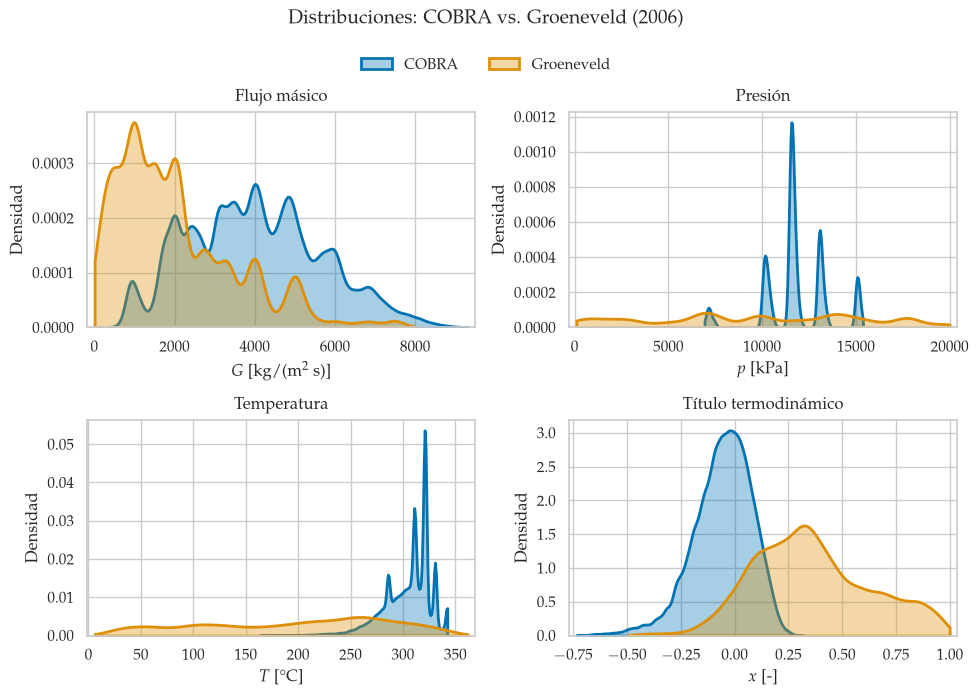
\includegraphics[width=\textwidth]{Figures/eda_cobra_groeneveld.png}
    \caption{Comparativa de distribuciones de datos de flujo másico, presión, temperatura y título termodinámico entre ensayos de un tubo de Groeneveld y todos los puntos de los ensayos numéricos con COBRA3-CP.}
    \label{fig:eda_cobra_groeneveld} 
\end{figure}

Entonces, se deben combinar los tensores de datos de entrenamiento de los datos de un tubo y de las simulaciones de COBRA3-CP para conformar el \texttt{Standard\allowbreak Scaler}. Las features adicionales que utiliza la red de alta fidelidad se escalan independientemente, por medio de un \texttt{Standard\allowbreak Scaler}. Para el valor del CHF también se pueden tener diferencias importantes, pero se realiza un escaleo independiente de las distribuciones, mediante la aplicación del logaritmo natural.

\subsection{Arquitectura del modelo}
Como se explicó previamente, el modelo planteado es una red de multifidelidad informada por física; se la denotará \texttt{MFPINN}. La \texttt{MFPINN} está compuesta por dos redes, una de baja fidelidad y otra de alta fidelidad. La de baja fidelidad es entrenada para predecir CHF en geometría de tubo, a partir de los datos crudos de las LUT de Groeneveld, y se la denotará \texttt{LFDNN}. Esta no tendrá información física, ya que se tiene una gran cantidad de datos, y un enfoque puro sobre ellos es suficiente. Su entrenamiento se realiza de forma previa, y sus pesos quedan congelados. Por otro lado, la componente de alta fidelidad sí utiliza información física, y se la denotará \texttt{HFPINN}. Los datos para su entrenamiento serán las simulaciones con COBRA3-CP de los ensayos experimentales de la Universidad de Columbia. En la figura \ref{fig:mfpinn} se presenta un esquema de la arquitectura de \texttt{MFPINN} explicada.

% Red neuronal multifidelidad:
%   - red de baja fidelidad (BF) pre-entrenada, con pesos fijos, que usa solo el
%     subconjunto de entradas x_1..x_n;
%   - red de alta fidelidad (AF) informada por la fisica (PINN), que usa todas las
%     entradas x_1..x_N mas la prediccion u_BF.
% La columna de entradas se dibuja UNA sola vez y es compartida: las entradas del
% subconjunto (recuadro sombreado) salen dos veces, hacia la red BF y hacia el bus
% de todas las entradas, mientras que las restantes salen solo hacia el bus.
%
% Fragmento para \input directo (sin el paquete standalone).
% NO necesita ninguna libreria de TikZ: solo \usepackage{tikz} y \usepackage{amsmath}.
% Uso tipico:
%   \begin{figure}[htbp]\centering
%     \resizebox{\textwidth}{!}{% Red neuronal multifidelidad:
%   - red de baja fidelidad (BF) pre-entrenada, con pesos fijos, que usa solo el
%     subconjunto de entradas x_1..x_n;
%   - red de alta fidelidad (AF) informada por la fisica (PINN), que usa todas las
%     entradas x_1..x_N mas la prediccion u_BF.
% La columna de entradas se dibuja UNA sola vez y es compartida: las entradas del
% subconjunto (recuadro sombreado) salen dos veces, hacia la red BF y hacia el bus
% de todas las entradas, mientras que las restantes salen solo hacia el bus.
%
% Fragmento para \input directo (sin el paquete standalone).
% NO necesita ninguna libreria de TikZ: solo \usepackage{tikz} y \usepackage{amsmath}.
% Uso tipico:
%   \begin{figure}[htbp]\centering
%     \resizebox{\textwidth}{!}{\input{Figures/mfnn_pinn.tex}}
%     \caption{...}\label{fig:mfnn_pinn}
%   \end{figure}
%
% Notas de implementacion (todas para que el fragmento no dependa del preambulo):
%  - Sin \usetikzlibrary aqui adentro: ejecutado en modo horizontal (dentro de un
%    \resizebox) deja ~55pt de espacios que ensanchan la caja del \input y hacen que
%    \resizebox empequenezca el dibujo; y no se puede encerrar en un grupo o \hbox
%    para absorberlos porque las definiciones de las librerias son locales.
%  - Sin la libreria backgrounds: los recuadros de las entradas se dibujan ANTES que
%    los circulos, de modo que el relleno queda debajo sin necesidad de capas.
%  - Sin la libreria fit: los recuadros de las redes se dan por coordenadas explicitas.
%  - Sin la libreria arrows.meta: las puntas son `stealth`, que ya trae pgf. Ademas se
%    escriben como -stealth y no con la clave >=, para no depender de que babel-spanish
%    tenga desactivado el shorthand `>`.
%  - Los tamanos de fuente son absolutos (\fontsize) para que la geometria no dependa
%    del tamano base del documento que hace el \input.
%  - El dibujo es casi cuadrado (15.3 x 15.3 cm) para que al escalarlo al ancho del
%    texto las etiquetas no queden diminutas.
\begin{figure}[hbtp]
  \centering
  \resizebox{\textwidth}{!}{
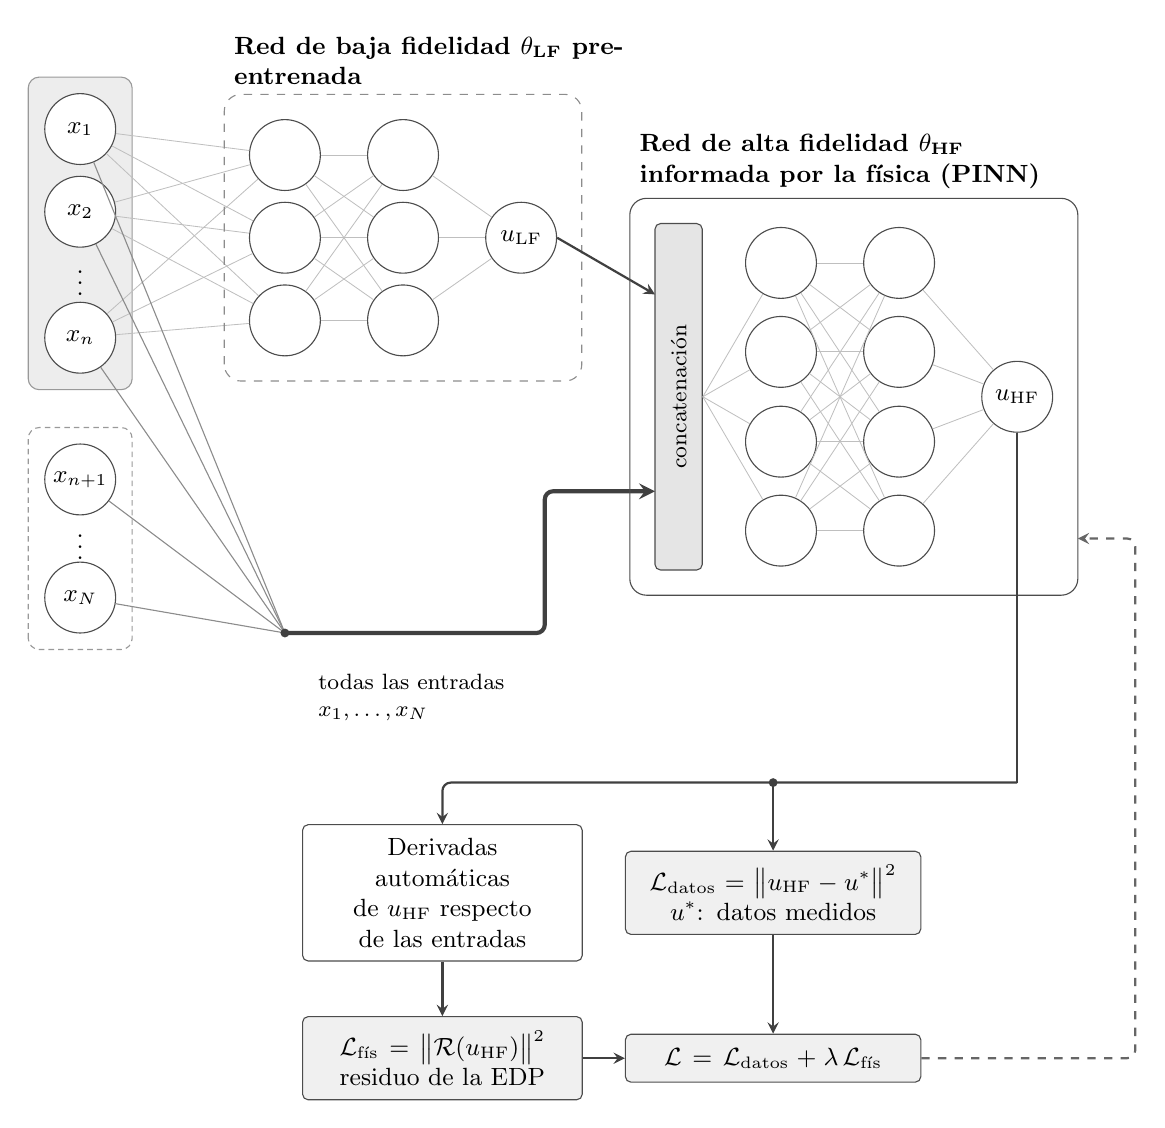
\begin{tikzpicture}[
  chico/.style={font=\fontsize{9}{11}\selectfont},
  % un unico estilo de circulo: entradas, neuronas y salidas miden todas lo mismo
  entrada/.style={circle,draw=black!70,fill=white,minimum size=0.9cm,inner sep=0pt,
                  font=\fontsize{9}{11}\selectfont},
  entradaG/.style={entrada},
  neurona/.style={entrada},
  salida/.style={entrada},
  syn/.style={draw=black!25,line width=0.3pt},
  reparto/.style={draw=black!45,line width=0.4pt},
  flujo/.style={-stealth,draw=black!75,line width=0.8pt},
  tronco/.style={draw=black!75,line width=0.8pt},
  bus/.style={-stealth,draw=black!75,line width=1.5pt},
  bloque/.style={rounded corners=2pt,draw=black!70,align=center,inner sep=5pt,
                 font=\fontsize{9}{11}\selectfont,text width=3.2cm},
  perdida/.style={bloque,fill=black!6},
  barra/.style={rounded corners=2pt,draw=black!70,fill=black!10,
                minimum width=0.6cm,minimum height=4.4cm,inner sep=0pt},
  grupoSub/.style={rounded corners=4pt,draw=black!40,fill=black!7},
  grupoResto/.style={rounded corners=4pt,draw=black!40,dash pattern=on 2pt off 1.5pt},
  grupoBF/.style={draw=black!45,dashed,rounded corners=6pt},
  grupoAF/.style={draw=black!70,rounded corners=6pt},
  etiqueta/.style={font=\fontsize{9}{11}\bfseries\selectfont,align=left,text width=5.2cm},
  nota/.style={font=\fontsize{8}{9.6}\selectfont,align=left},
  notac/.style={font=\fontsize{8}{9.6}\selectfont,align=center},
  bp/.style={-stealth,dashed,draw=black!60,line width=0.8pt},
]

%=============== COLUMNA DE ENTRADAS (UNICA Y COMPARTIDA) ==============
% los recuadros van primero para que el relleno quede por debajo de los circulos
\draw[grupoSub]   (-0.66, 0.09) rectangle (0.66, 4.06);
\draw[grupoResto] (-0.66,-3.21) rectangle (0.66,-0.39);

% subconjunto que ve la red de baja fidelidad
\node[entrada]  (e1)  at (0, 3.40) {$x_1$};
\node[entrada]  (e2)  at (0, 2.35) {$x_2$};
\node[chico]    (ev1) at (0, 1.55) {$\vdots$};
\node[entrada]  (en)  at (0, 0.75) {$x_n$};
% entradas restantes, exclusivas de la red de alta fidelidad
\node[entradaG] (er1) at (0,-1.05) {$x_{n+1}$};
\node[chico]    (ev2) at (0,-1.80) {$\vdots$};
\node[entrada]  (eN)  at (0,-2.55) {$x_N$};

% \node[notac,rotate=90] at (-1.35, 2.02) {primeras $n$\\ entradas};
% \node[notac,rotate=90] at (-1.35,-1.80) {entradas\\ restantes};

%=================== RED DE BAJA FIDELIDAD (BF) ========================
\foreach \j/\y in {1/3.07,2/2.02,3/0.97} {
  \node[neurona] (bf1-\j) at (2.6,\y) {};
  \node[neurona] (bf2-\j) at (4.1,\y) {};
}
\node[salida] (ubf) at (5.6,2.02) {$u_\text{LF}$};

% solo el subconjunto alimenta la red BF
\foreach \e in {e1,e2,en} {
  \foreach \j in {1,2,3} { \draw[syn] (\e) -- (bf1-\j); }
}
\foreach \i in {1,2,3} {
  \foreach \j in {1,2,3} { \draw[syn] (bf1-\i) -- (bf2-\j); }
  \draw[syn] (bf2-\i) -- (ubf);
}

\draw[grupoBF] (1.83,0.20) rectangle (6.37,3.84);
\node[etiqueta,anchor=south west] at (1.83,3.84)
  {Red de baja fidelidad $\theta_\text{LF}$ pre-entrenada};

%=========== BUS CON TODAS LAS ENTRADAS HACIA LA RED AF ================
% cada entrada, del subconjunto y de las restantes, se reparte al bus
\coordinate (nodoBus) at (2.6,-3.0);
\foreach \e in {e1,e2,en,er1,eN} { \draw[reparto] (\e) -- (nodoBus); }
\fill[black!75] (nodoBus) circle (1.6pt);

\draw[bus,rounded corners=3pt] (nodoBus) -- (5.9,-3.0) -- (5.9,-1.2) -- (7.30,-1.2);
\node[nota,anchor=north west] at (2.9,-3.4) {todas las entradas\\ $x_1,\dots,x_N$};

%=================== RED DE ALTA FIDELIDAD (AF) ========================
\node[barra] (concat) at (7.6,0) {};
\node[nota,rotate=90] at (7.6,0) {concatenación};

\foreach \j/\y in {1/1.70,2/0.57,3/-0.57,4/-1.70} {
  \node[neurona] (af1-\j) at (8.9,\y) {};
  \node[neurona] (af2-\j) at (10.4,\y) {};
}
\node[salida] (uaf) at (11.9,0) {$u_\text{HF}$};

\draw[flujo] (ubf.east) -- (7.30,1.3);
\foreach \j in {1,2,3,4} { \draw[syn] (concat.east) -- (af1-\j); }
\foreach \i in {1,2,3,4} {
  \foreach \j in {1,2,3,4} { \draw[syn] (af1-\i) -- (af2-\j); }
  \draw[syn] (af2-\i) -- (uaf);
}

\draw[grupoAF] (6.98,-2.52) rectangle (12.67,2.52);
\node[etiqueta,anchor=south west] at (6.98,2.52)
  {Red de alta fidelidad $\theta_\text{HF}$\\ informada por la física (PINN)};

%=============== RAMAS DE PÉRDIDA (FÍSICA Y DATOS) =====================
\node[bloque]  (ad)   at (4.6,-6.3)
  {Derivadas\\ automáticas\\ de $u_\text{HF}$ respecto\\ de las entradas};
\node[perdida] (lfis) at (4.6,-8.4)
  {$\mathcal{L}_{\text{fís}}=\big\|\mathcal{R}(u_\text{HF})\big\|^{2}$\\ residuo de la EDP};
\node[perdida,text width=3.4cm] (ldat) at (8.8,-6.3)
  {$\mathcal{L}_{\text{datos}}=\big\|u_\text{HF}-u^{*}\big\|^{2}$\\ $u^{*}$: datos medidos};
\node[perdida,text width=3.4cm] (ltot) at (8.8,-8.4)
  {$\mathcal{L}=\mathcal{L}_{\text{datos}}+\lambda\,\mathcal{L}_{\text{fís}}$};

% tronco desde u_AF, con derivacion hacia la rama de datos
\coordinate (bif) at (11.9,-4.9);
\draw[tronco] (uaf.south) -- (bif);
\draw[flujo,rounded corners=3pt] (bif) -- (4.6,-4.9) -- (ad.north);
\fill[black!75] (8.8,-4.9) circle (1.6pt);
\draw[flujo] (8.8,-4.9) -- (ldat.north);

\draw[flujo] (ad.south)   -- (lfis.north);
\draw[flujo] (ldat.south) -- (ltot.north);
\draw[flujo] (lfis.east)  -- (ltot.west);

%=================== RETROPROPAGACIÓN (SOLO RED AF) ====================
% vuelve por la derecha y entra al costado de la red AF, sin cruzar el tronco
\draw[bp,rounded corners=3pt]
  (ltot.east) -- (13.4,-8.4) -- (13.4,-1.8) -- (12.67,-1.8);
% \node[notac,anchor=north,text width=4.2cm] at (8.8,-9.3)
%   {retropropagación: sólo se\\ actualizan los pesos $\theta_{AF}$};

%============================ ACLARACIÓN ===============================
% \node[nota,anchor=north west,text width=4.0cm] at (-1.75,-4.9)
%   {la red BF sólo usa $x_1,\dots,x_n$; la red AF usa todas las entradas y
%    además $u_{BF}$};

\end{tikzpicture}
  }
  \caption{Esquema de la arquitectura de red neuronal de multifidelidad informada por física.}
  \label{fig:mfpinn}
\end{figure}
}
%     \caption{...}\label{fig:mfnn_pinn}
%   \end{figure}
%
% Notas de implementacion (todas para que el fragmento no dependa del preambulo):
%  - Sin \usetikzlibrary aqui adentro: ejecutado en modo horizontal (dentro de un
%    \resizebox) deja ~55pt de espacios que ensanchan la caja del \input y hacen que
%    \resizebox empequenezca el dibujo; y no se puede encerrar en un grupo o \hbox
%    para absorberlos porque las definiciones de las librerias son locales.
%  - Sin la libreria backgrounds: los recuadros de las entradas se dibujan ANTES que
%    los circulos, de modo que el relleno queda debajo sin necesidad de capas.
%  - Sin la libreria fit: los recuadros de las redes se dan por coordenadas explicitas.
%  - Sin la libreria arrows.meta: las puntas son `stealth`, que ya trae pgf. Ademas se
%    escriben como -stealth y no con la clave >=, para no depender de que babel-spanish
%    tenga desactivado el shorthand `>`.
%  - Los tamanos de fuente son absolutos (\fontsize) para que la geometria no dependa
%    del tamano base del documento que hace el \input.
%  - El dibujo es casi cuadrado (15.3 x 15.3 cm) para que al escalarlo al ancho del
%    texto las etiquetas no queden diminutas.
\begin{figure}[hbtp]
  \centering
  \resizebox{\textwidth}{!}{
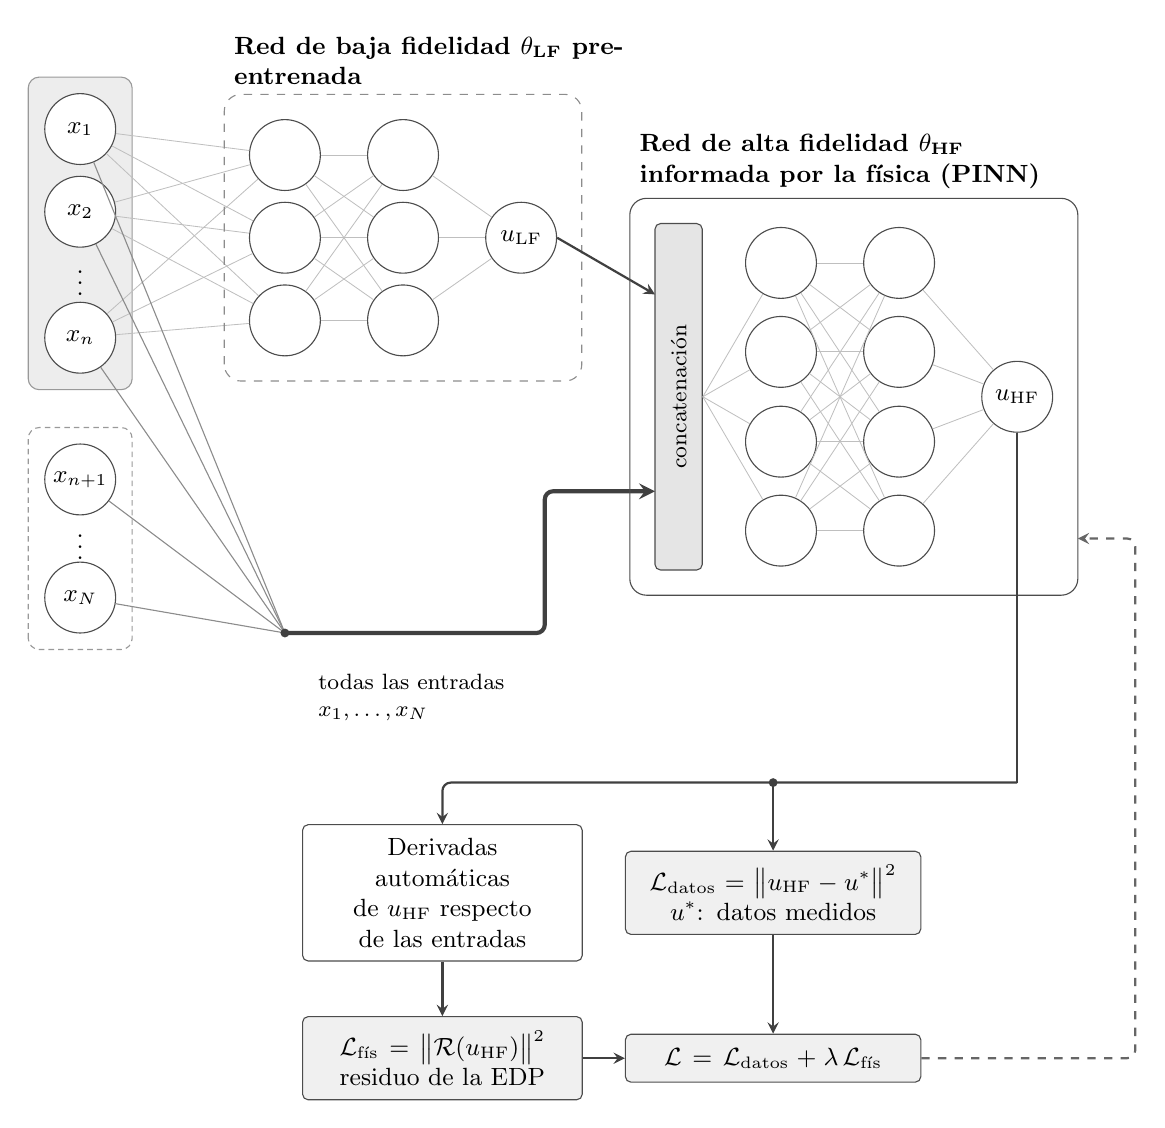
\begin{tikzpicture}[
  chico/.style={font=\fontsize{9}{11}\selectfont},
  % un unico estilo de circulo: entradas, neuronas y salidas miden todas lo mismo
  entrada/.style={circle,draw=black!70,fill=white,minimum size=0.9cm,inner sep=0pt,
                  font=\fontsize{9}{11}\selectfont},
  entradaG/.style={entrada},
  neurona/.style={entrada},
  salida/.style={entrada},
  syn/.style={draw=black!25,line width=0.3pt},
  reparto/.style={draw=black!45,line width=0.4pt},
  flujo/.style={-stealth,draw=black!75,line width=0.8pt},
  tronco/.style={draw=black!75,line width=0.8pt},
  bus/.style={-stealth,draw=black!75,line width=1.5pt},
  bloque/.style={rounded corners=2pt,draw=black!70,align=center,inner sep=5pt,
                 font=\fontsize{9}{11}\selectfont,text width=3.2cm},
  perdida/.style={bloque,fill=black!6},
  barra/.style={rounded corners=2pt,draw=black!70,fill=black!10,
                minimum width=0.6cm,minimum height=4.4cm,inner sep=0pt},
  grupoSub/.style={rounded corners=4pt,draw=black!40,fill=black!7},
  grupoResto/.style={rounded corners=4pt,draw=black!40,dash pattern=on 2pt off 1.5pt},
  grupoBF/.style={draw=black!45,dashed,rounded corners=6pt},
  grupoAF/.style={draw=black!70,rounded corners=6pt},
  etiqueta/.style={font=\fontsize{9}{11}\bfseries\selectfont,align=left,text width=5.2cm},
  nota/.style={font=\fontsize{8}{9.6}\selectfont,align=left},
  notac/.style={font=\fontsize{8}{9.6}\selectfont,align=center},
  bp/.style={-stealth,dashed,draw=black!60,line width=0.8pt},
]

%=============== COLUMNA DE ENTRADAS (UNICA Y COMPARTIDA) ==============
% los recuadros van primero para que el relleno quede por debajo de los circulos
\draw[grupoSub]   (-0.66, 0.09) rectangle (0.66, 4.06);
\draw[grupoResto] (-0.66,-3.21) rectangle (0.66,-0.39);

% subconjunto que ve la red de baja fidelidad
\node[entrada]  (e1)  at (0, 3.40) {$x_1$};
\node[entrada]  (e2)  at (0, 2.35) {$x_2$};
\node[chico]    (ev1) at (0, 1.55) {$\vdots$};
\node[entrada]  (en)  at (0, 0.75) {$x_n$};
% entradas restantes, exclusivas de la red de alta fidelidad
\node[entradaG] (er1) at (0,-1.05) {$x_{n+1}$};
\node[chico]    (ev2) at (0,-1.80) {$\vdots$};
\node[entrada]  (eN)  at (0,-2.55) {$x_N$};

% \node[notac,rotate=90] at (-1.35, 2.02) {primeras $n$\\ entradas};
% \node[notac,rotate=90] at (-1.35,-1.80) {entradas\\ restantes};

%=================== RED DE BAJA FIDELIDAD (BF) ========================
\foreach \j/\y in {1/3.07,2/2.02,3/0.97} {
  \node[neurona] (bf1-\j) at (2.6,\y) {};
  \node[neurona] (bf2-\j) at (4.1,\y) {};
}
\node[salida] (ubf) at (5.6,2.02) {$u_\text{LF}$};

% solo el subconjunto alimenta la red BF
\foreach \e in {e1,e2,en} {
  \foreach \j in {1,2,3} { \draw[syn] (\e) -- (bf1-\j); }
}
\foreach \i in {1,2,3} {
  \foreach \j in {1,2,3} { \draw[syn] (bf1-\i) -- (bf2-\j); }
  \draw[syn] (bf2-\i) -- (ubf);
}

\draw[grupoBF] (1.83,0.20) rectangle (6.37,3.84);
\node[etiqueta,anchor=south west] at (1.83,3.84)
  {Red de baja fidelidad $\theta_\text{LF}$ pre-entrenada};

%=========== BUS CON TODAS LAS ENTRADAS HACIA LA RED AF ================
% cada entrada, del subconjunto y de las restantes, se reparte al bus
\coordinate (nodoBus) at (2.6,-3.0);
\foreach \e in {e1,e2,en,er1,eN} { \draw[reparto] (\e) -- (nodoBus); }
\fill[black!75] (nodoBus) circle (1.6pt);

\draw[bus,rounded corners=3pt] (nodoBus) -- (5.9,-3.0) -- (5.9,-1.2) -- (7.30,-1.2);
\node[nota,anchor=north west] at (2.9,-3.4) {todas las entradas\\ $x_1,\dots,x_N$};

%=================== RED DE ALTA FIDELIDAD (AF) ========================
\node[barra] (concat) at (7.6,0) {};
\node[nota,rotate=90] at (7.6,0) {concatenación};

\foreach \j/\y in {1/1.70,2/0.57,3/-0.57,4/-1.70} {
  \node[neurona] (af1-\j) at (8.9,\y) {};
  \node[neurona] (af2-\j) at (10.4,\y) {};
}
\node[salida] (uaf) at (11.9,0) {$u_\text{HF}$};

\draw[flujo] (ubf.east) -- (7.30,1.3);
\foreach \j in {1,2,3,4} { \draw[syn] (concat.east) -- (af1-\j); }
\foreach \i in {1,2,3,4} {
  \foreach \j in {1,2,3,4} { \draw[syn] (af1-\i) -- (af2-\j); }
  \draw[syn] (af2-\i) -- (uaf);
}

\draw[grupoAF] (6.98,-2.52) rectangle (12.67,2.52);
\node[etiqueta,anchor=south west] at (6.98,2.52)
  {Red de alta fidelidad $\theta_\text{HF}$\\ informada por la física (PINN)};

%=============== RAMAS DE PÉRDIDA (FÍSICA Y DATOS) =====================
\node[bloque]  (ad)   at (4.6,-6.3)
  {Derivadas\\ automáticas\\ de $u_\text{HF}$ respecto\\ de las entradas};
\node[perdida] (lfis) at (4.6,-8.4)
  {$\mathcal{L}_{\text{fís}}=\big\|\mathcal{R}(u_\text{HF})\big\|^{2}$\\ residuo de la EDP};
\node[perdida,text width=3.4cm] (ldat) at (8.8,-6.3)
  {$\mathcal{L}_{\text{datos}}=\big\|u_\text{HF}-u^{*}\big\|^{2}$\\ $u^{*}$: datos medidos};
\node[perdida,text width=3.4cm] (ltot) at (8.8,-8.4)
  {$\mathcal{L}=\mathcal{L}_{\text{datos}}+\lambda\,\mathcal{L}_{\text{fís}}$};

% tronco desde u_AF, con derivacion hacia la rama de datos
\coordinate (bif) at (11.9,-4.9);
\draw[tronco] (uaf.south) -- (bif);
\draw[flujo,rounded corners=3pt] (bif) -- (4.6,-4.9) -- (ad.north);
\fill[black!75] (8.8,-4.9) circle (1.6pt);
\draw[flujo] (8.8,-4.9) -- (ldat.north);

\draw[flujo] (ad.south)   -- (lfis.north);
\draw[flujo] (ldat.south) -- (ltot.north);
\draw[flujo] (lfis.east)  -- (ltot.west);

%=================== RETROPROPAGACIÓN (SOLO RED AF) ====================
% vuelve por la derecha y entra al costado de la red AF, sin cruzar el tronco
\draw[bp,rounded corners=3pt]
  (ltot.east) -- (13.4,-8.4) -- (13.4,-1.8) -- (12.67,-1.8);
% \node[notac,anchor=north,text width=4.2cm] at (8.8,-9.3)
%   {retropropagación: sólo se\\ actualizan los pesos $\theta_{AF}$};

%============================ ACLARACIÓN ===============================
% \node[nota,anchor=north west,text width=4.0cm] at (-1.75,-4.9)
%   {la red BF sólo usa $x_1,\dots,x_n$; la red AF usa todas las entradas y
%    además $u_{BF}$};

\end{tikzpicture}
  }
  \caption{Esquema de la arquitectura de red neuronal de multifidelidad informada por física.}
  \label{fig:mfpinn}
\end{figure}


La \texttt{HFPINN} entrena con los datos de las simulaciones con COBRA3-CP; cada una de ellas provee datos en 151 nodos axiales y 60 subcanales, para un total de 9060 datos por ensayo. Por otro lado, la información provista por los ensayos de Columbia provee 1 dato por ensayo, correspondiente al punto, desconocido, en el que comienza el DNB. Se tiene entonces un desajuste de dimensionalidad entre el producto de la red al evaluar en los ensayos numéricos y lo medido en los ensayos reales:
\begin{equation}
    \underbrace{\mathbf{y} \in \mathbb{R}^{9060}}_{\text{campo predicho}}
    \quad\longrightarrow\quad
    \underbrace{\hat{y} \in \mathbb{R}}_{\text{campo medido}}.
    \label{eq:dim_red}
\end{equation}
La flecha en la ecuación \ref{eq:dim_red} es la reducción de dimensionalidad que se debe hacer antes de poder comparar contra los datos experimentales. La elección natural es el mínimo, ya que el DNB ocurre en el nodo más limitante del bundle. Pero, en cuanto a la optimización numérica, la utilización del mínimo es poco eficiente, e incluso puede hacer imposible el entrenamiento de un modelo de red neuronal, ya que el mínimo genera un gradiente \textit{one-hot}:
\begin{equation}
    \frac{\partial}{\partial y_j}\min_i y_i =
    \begin{cases}
    1 & \text{si } j = \arg\min_i y_i \\
    0 & \text{en caso contrario}
    \end{cases}.
\end{equation}
De esta forma el optimizador sólo recibe información del punto mínimo. Adicionalmente, al comenzar el entrenamiento, el punto que resulta mínimo es completamente aleatorio, por lo que es muy fácil condicionar negativamente la red y que esta no pueda salir del mínimo inicial.

Se plantea entonces utilizar un enfoque de mínimo suave o \textit{softmin}, que permita utilizar una mayor cantidad de nodos para el aprendizaje. Un problema similar que utiliza este enfoque es el promedio ponderado o \textit{attention pooling} propuesto por Ilse \citep{ilse2018attention} en el contexto de MIL (del inglés, \textit{Multiple Instance Learning}). Se propone utilizar un softmin de la forma:
\begin{equation}
    \mathrm{softmin}_\tau (\mathbf{y}) = \sum_i w_i y_i,
\end{equation}
donde $w_i$ son los pesos para ponderar las distintas predicciones. En el trabajo de Ilse los pesos se aprenden con una red de atención aparte, pero en este trabajo se utiliza el propio campo predicho, a través de la función softmax de Bridle \citep{bridle1990softmax} y el parámetro de temperatura propuesto por Hinton, Vinyals y Dean \citep{hinton2015distilling}:
\begin{equation}
    w_i = \mathrm{softmax}\left(-\frac{\mathbf{y}}{\tau}\right)_i .
\end{equation}
De esta forma, los nodos con baja predicción se ponderan con un mayor peso que los nodos con predicciones altas. El sesgo de esta concentración es controlado por el parámetro de temperatura $\tau$, que viene dado a partir del desvío estándar del vector de predicción:
\begin{equation}
    \tau = \alpha \cdot \mathrm{std}(\mathbf{y}).
\end{equation}
El parámetro $\alpha$ permite controlar la temperatura con la evolución del entrenamiento, y se lo controla por medio de un recocido o \textit{annealing}, que lo recorre geométricamente desde $\alpha_0$ hasta $\alpha_f$.

Para evaluar si la temperatura $\tau$ a la que converge el entrenamiento es o no correcta, se debe analizar sobre cuántos nodos se está promediando realmente. Para ello, se computa el número efectivo de nodos, que viene dado por la exponencial de la entropía de los pesos:
\begin{equation}
    N_\mathrm{eff} = \exp\left[ -\sum_i w_i\,\log(w_i) \right].
\end{equation}
Esta definición es el número de Hill de orden 1 \citep{hill1973diversity}, la forma estándar de obtener un conteo efectivo a partir de una entropía. Si el entrenamiento es satisfactorio, $N_\mathrm{eff}$ debe ser menor a 5 para su final.

Esta metodología, además de solucionar el problema del gradiente one-hot, tiene la ventaja de, al ser una combinación convexa de los $y_i$, estar acotada superiormente por la media de la predicción. Esto asegura que el valor predicho sea un valor físicamente válido y sin sesgo dependiente de la cantidad de nodos utilizados.

En cuanto a la información física que se le brindará a la \texttt{HFPINN}, se debe notar que no es posible hacer un planteo tradicional de PINN que provea una ecuación diferencial de conservación de alguna cantidad como función de pérdida. Esto es así puesto que la variable a predecir, el CHF, no responde a una ecuación de conservación, sino que es una propiedad del estado termodinámico y la geometría. Se podría realizar el ejercicio de proveer a la red de, por ejemplo, la ecuación de conservación de la energía. Esto haría que la red aprenda que siempre que le den un set de datos locales, los mismos corresponden a una condición de CHF, ya que la red fue entrenada con casos en que se tiene DNB. Pero en el campo de aplicación del modelo, se busca estimar el CHF sin estar en DNB.

Se plantean entonces, distintos tipos de ecuaciones diferenciales a satisfacer por el modelo. Se tendrán relaciones monotónicas, de derivada cruzada, de convexidad y de coincidencia entre la predicción del modelo y la simulación de COBRA3-CP.

Las relaciones monotónicas del CHF con las variables de entrada implementadas son: positiva con el flujo másico, negativa con el título termodinámico y negativa con la presión. Estas relaciones tienen fundamento físico y aseguran que las salidas de la red en condiciones de extrapolación mantengan sentido físico. Vale aclarar que esta última es válida para el rango de aplicación de reactores PWR o PHWR, es decir, por encima de 100 bar.

Se implementa una relación negativa con la derivada cruzada respecto del flujo másico y el título termodinámico, fundamentada en que a mayor flujo másico, la caída del CHF con el título termodinámico es más pronunciada. Esto es consistente con las estimaciones de las LUT de Groeneveld.

En cuanto a la relación de convexidad, se plantea una derivada segunda positiva del CHF respecto del título termodinámico para la zona de alto título ($x>0,2$). Si bien de la figura \ref{fig:eda_cobra_groeneveld} puede afirmarse que se tienen pocos datos que se encuentran en esa región, esta restricción es útil en puntos de colocación para asegurar que el modelo no obtiene resultados indeseados al extrapolar fuera de los datos de entrenamiento.

Por último, se realiza la comparación de la derivada axial del valor predicho de CHF calculada por dos métodos. En primer lugar se computa la derivada observada como:
\begin{equation}
    \left. \frac{d\mathrm{CHF}}{dz} \right|_\text{obs} = \frac{\mathrm{CHF}_{z_{i+1}} - \mathrm{CHF}_{z_{i}}}{z_{i+1} - z_i}.
\end{equation}
Luego la derivada por regla de la cadena viene dada por:
\begin{equation}
    \left. \frac{d\mathrm{CHF}}{dz} \right|_\text{cadena} = \sum_{j\in\mathrm{feats}} \frac{\partial \mathrm{CHF}}{\partial j} \frac{dj}{dz} ,
\end{equation}
donde las derivadas de las variables respecto de la coordenada axial $\nicefrac{dj}{dz}$ fueron computadas previamente a partir de los resultados de las simulaciones con COBRA3-CP. De esta manera se penaliza que la red invente dependencias axiales que no provengan de las condiciones locales, y de alguna forma, es una expresión de la hipótesis de condiciones locales como PDE.

Para el entrenamiento del modelo, en primer lugar se entrena la \texttt{LFDNN} con sus datos. Su entrenamiento es estándar y puede realizarse con optimizador Adam y métrica MSE.
Luego, con los pesos de la \texttt{LFDNN} congelados, se entrena la \texttt{HFPINN} con la estructura completa de la \texttt{MFPINN}. Para ello se realizaron pruebas para determinar si es necesario, debido a las restricciones tipo PINN, un optimizador de segundo orden como L-BFGS \citep{liu1989lbfgs}. El resultado de las mismas se expone en el capítulo \ref{Chapter4}.

\subsection{Evaluación del modelo}
Para la evaluación del modelo se utilizaron las métricas estadísticas tradicionales en conjunto con métricas particulares al problema en particular. Las métricas estadísticas utilizadas son el error cuadrático medio (MSE, del inglés \textit{Mean Squared Error}), su raíz (RMSE, del inglés \textit{Root Mean Squared Error}), y el coeficiente de correlación $\mathrm{R}^2$. En cuanto a la métricas particulares al problema, se utiliza el $\mathrm{DNBR}_\mathrm{min}$ del diseño termohidráulico de la \cna{}, explicado en detalle en \citep{IFS_CNA2, invap_thdesign}. Este es el valor para el cual, si la predicción de DNBR está por encima, se asegura con 95\% de probabilidad y confianza que no se tiene DNB. Se define como:
\begin{equation}
    \mathrm{DNBR}_\mathrm{min} = \overline{\mathrm{DNBR}} + k_{95}\cdot \sigma(\mathrm{DNBR}) ,
\end{equation}
donde DNBR son las predicciones en las condiciones de los ensayos de la Universidad de Columbia, y $k_{95}$ es el intervalo de tolerancia de una distribución normal para asegurar 95\% de probabilidad y confianza según la cantidad de observaciones \citep{nist_e_handbook_tolerance}. Se compara con la metodología actual (LUT + TMF), que obtiene $\mathrm{DNBR}_\mathrm{min} = 1,21$.
% Chapter Template

\chapter{Ensayos y resultados} % Main chapter title
\label{Chapter4}
En este capítulo se presentan los resultados de los estudios realizados sobre los modelos de predicción de PLC y CHF. 

\section{Estimación de PLC}
A continuación, se presentan los resultados para el modelo de estimación de PLC: la optimización de hiperparámetros, las predicciones de DNBR y fracción de vacío del mejor modelo y la estimación de PLC por ambos criterios.

\subsection{Optimización de hiperparámetros}
Como se mencionó en la sección \ref{sec:plc_arq}, la optimización de hiperparámetros se realizó por medio de la biblioteca Optuna. Las métricas objetivo se establecieron por separado para cada criterio. Para el DNBR se utilizó el error porcentual medio, mientras que para la fracción de vacío se usó el error absoluto medio escalado 100 veces. Esta decisión se tomó al considerar que la fracción de vacío tiene valor exactamente igual a 0 para un porcentaje importante de los datos y con el objetivo de lograr una contribución equitativa de ambos criterios al rendimiento del modelo. De esta forma, se obtiene un único modelo con error similar en ambos criterios y se evita entrenar uno por cada uno de ellos.

La figura \ref{fig:plc_opt_results} muestra los resultados durante el proceso de optimización, mientras que la arquitectura final se resume en la tabla \ref{tab:plc_arq_hp}.

\begin{table}[H]
	\centering
	\caption{Hiperparámetros de la arquitectura final.}
	\begin{tabular}{l c}    
        \toprule
        \textbf{Hiperparámetro} & \textbf{Valor} \\
        \hline
        Cantidad de capas ocultas & $3$ \\
        Cantidad de neuronas por capa & $478$ \\
        Learning rate & $1.38 \cdot 10^{-4}$ \\
        Batch & 64 \\
        Función de activación & ReLU \\
		\bottomrule
	\end{tabular}
	\label{tab:plc_arq_hp}
\end{table}

\begin{figure}[H]
    \centering
    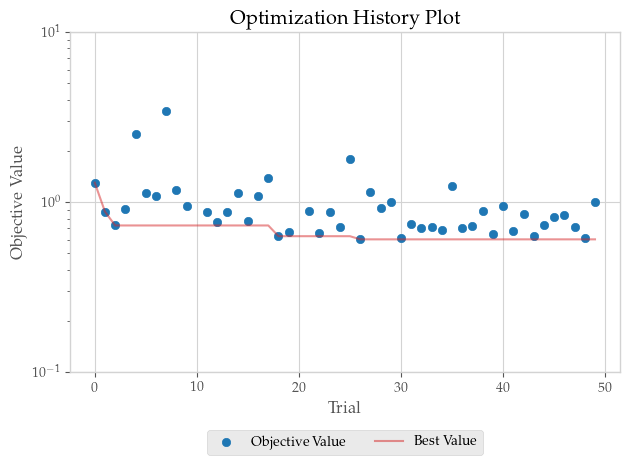
\includegraphics[width=0.7\textwidth]{Figures/plc_opt_result.png}
    \caption{Resultados de los distintos intentos de la optimización.}
    \label{fig:plc_opt_results}
\end{figure}

\subsection{Resultados de DNBR y fracción de vacío}

En esta sección, se evalúan los resultados del modelo en cuanto a la predicción de DNBR y fracción de vacío. En la figura \ref{fig:plc_results_dnbr_vacio} se presentan los gráficos de valores predichos contra reales, para los conjuntos de test y train. Se observa una buena predicción del modelo en ambos objetivos y una distribución equivalente entre conjuntos. No obstante, se aprecia una tendencia a subestimar la fracción de vacío en la región cercana a 25\%.

\begin{figure}[h]
    \centering
    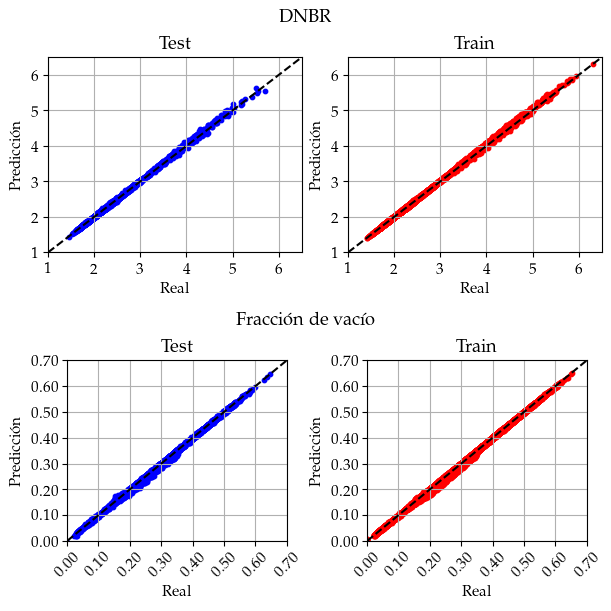
\includegraphics[width=0.8\textwidth]{Figures/plc_pred.png}
    \caption{Resultados de predicción de DNBR y fracción de vacío, para los conjuntos de test y train.}
    \label{fig:plc_results_dnbr_vacio}
\end{figure}

En la tabla \ref{tab:plc_errors_dnbr_vacio} se presentan la media y el desvío estándar del error con signo para cada objetivo. El error con signo se define como la diferencia entre el valor real y el predicho, por lo que valores positivos de la media implican una subpredicción del objetivo, y los negativos una sobrepredicción. Para la fracción de vacío, se aplica un factor de 10 para que las magnitudes entre objetivos sean comparables. Se observa una tendencia a subpredecir DNBR y a sobrepredecir la fracción de vacío, ambas tendencias en igual magnitud en train y test. Los desvíos estándar son menores en test que en train para DNBR, y a la inversa para la fracción de vacío. En ambos casos, los valores de desvío estándar son bajos. 

La tendencia general de la predicción de vacío es a sobrepredecir, mientras que el gráfico de predicho contra real indica lo contrario. Para analizar esta discrepancia, se realizó el mismo cálculo del error al dividir en 5 regiones el dominio de cada variable objetivo. Los resultados se presentan en la tabla \ref{tab:plc_errors_dnbr_vacio_segmentado}. Se obtiene, para DNBR, una media aún más baja en la región de interés ($1.7-2.5$) y una subpredicción general del DNBR, lo que representa una tendencia conservativa. En cuanto a la fracción de vacío, no se tiene el mínimo de error en la zona de interés, sino alrededor de ella. En la zona de interés ($0.15-0.35$) se tiene una sobrepredicción de la fracción de vacío, también una tendencia conservativa. Se puede concluir entonces que el modelo tiene un buen rendimiento en ambos objetivos y tendencias conservativas respecto de las referencias.

\begin{table}[h]
	\centering
	\caption{Media y desvío estándar del error con signo para cada objetivo.}
	\begin{tabular}{c c c c c} 
        \toprule
        \multirow{2}{*}{\textbf{Conjunto}} & \multicolumn{2}{c}{\textbf{DNBR}} & \multicolumn{2}{c}{\textbf{Fracción de vacío}} \\
                & media     & $\sigma$  & media & $\sigma$  \\
        Train   & $-0.006$    & $0.021$     & $0.018$ & $0.040$     \\
        Test    & $-0.006$    & $0.017$     & $0.018$ & $0.032$     \\
		\bottomrule
	\end{tabular}
	\label{tab:plc_errors_dnbr_vacio}
\end{table}

\begin{table}[h]
	\centering
	\caption{Media y desvío estándar del error con signo para cada objetivo, segmentado por rangos de cada objetivo.}
	\begin{tabular}{c c c c c c} 
        \toprule
        \multirow{3}{1.5cm}{\textbf{Objetivo}} & \multirow{3}{*}{\textbf{Rango}} & \multicolumn{4}{c}{\textbf{Conjunto}} \\
        &                                               & \multicolumn{2}{c}{Train} & \multicolumn{2}{c}{Test} \\ 
        &                                               & media & $\sigma$  & media & $\sigma$  \\
        \multirow{5}{1.5cm}{DNBR}               
                        &$   <1.7$  & $0.003$ &   $0.004$   & $0.000$ &  $0.008$    \\ 
                        &$1.7-2.5$  & $-0.001$&   $0.009$   & $-0.001$&  $0.013$    \\
                        &$2.5-3.5$  & $-0.013$&   $0.013$   & $-0.015$&  $0.019$    \\
                        &$  3.5-5$  & $-0.044$&   $0.038$   & $-0.042$&  $0.051$    \\
                        &$     >5$  & $-0.051$&   $0.039$   & $-0.015$&  $0.076$    \\
        \hline
        \multirow{5}{1.5cm}{Fracción de vacío}
                        &$        0$  & $-0.035$ & $0.033$ & $0.061$ & $0.037$ \\ 
                        &$   0-0.15$  &  $0.013$ & $0.021$ & $0.010$ & $0.032$ \\
                        &$0.15-0.35$  &  $0.024$ & $0.036$ & $0.025$ & $0.044$ \\
                        &$ 0.35-0.6$  &  $0.007$ & $0.021$ & $0.007$ & $0.027$ \\
                        &$     >0.6$  &  $0.031$ & $0.022$ & $0.024$ & $0.014$ \\

		\bottomrule
	\end{tabular}
	\label{tab:plc_errors_dnbr_vacio_segmentado}
\end{table}

Como se explicó en la sección \ref{sec:plc_pipeline}, se filtraron los datos disponibles para entrenar en la región de interés en ambas variables objetivo. El filtro conservó los valores de MDNBR entre $1.7$ y $2.5$, o de fracción de vacío entre 15\% y 35\%. Por ello, resulta de interés evaluar la precisión del modelo por fuera de la región de entrenamiento. En la figura \ref{fig:plc_results_excluidos} se presentan las predicciones comparadas con los valores reales, para MDNBR y fracción de vacío.
En primer lugar, se evidencia la dificultad del modelo para predecir en las regiones excluidas del entrenamiento, algo esperable en una arquitectura DNN.
Luego, para DNBR se observa un comportamiento correcto en valores inferiores a los de interés, pero una tendencia a subpredecir al aumentar. Si bien esto podría interpretarse generalmente como un resultado desfavorable, se puede considerar que el modelo entrega predicciones conservativas fuera de su zona de entrenamiento y brinda seguridad en su aplicación. Por último, para la fracción de vacío, por debajo de la zona de interés se observan predicciones menores a 0, lo que constituye un resultado no físico. Se podría realizar un clipping de la predicción para que los valores negativos se conviertan en 0, lo que daría un buen rendimiento por debajo de la zona de entrenamiento. Por encima de la zona de entrenamiento, se puede observar en primer lugar una tendencia a subpredecir hasta 60\% y luego una sobrepredicción. 

Para cuantificar el aumento del error en el conjunto excluido, la figura \ref{fig:plc_errores} presenta los errores para cada variable objetivo en los conjuntos de train, test y excluidos. Tal como se comentó previamente, los conjuntos de train y test presentan errores muy similares, y el conjunto excluido un error considerablemente mayor. Adicionalmente, se grafican los cuantiles del 5\% y 95\%, que evidencian que el conjunto de excluidos también tiene una dispersión mucho mayor en su error.

\begin{figure}[H]
    \centering
    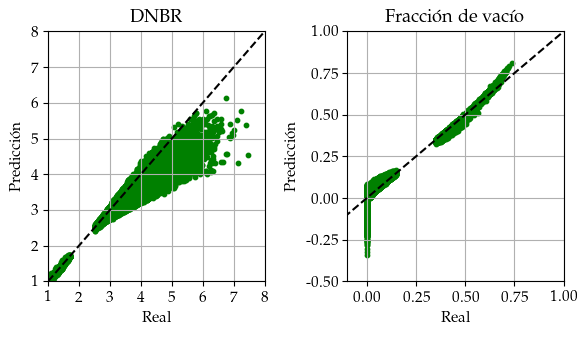
\includegraphics[width=0.8\textwidth]{Figures/plc_pred_excluidos.png}
    \caption{Resultados de predicción de DNBR y fracción de vacío, para el conjunto excluido.}
    \label{fig:plc_results_excluidos}
\end{figure}

\begin{figure}[H]
    \centering
    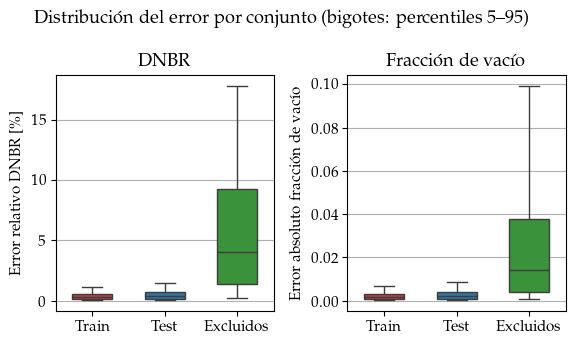
\includegraphics[width=0.8\textwidth]{Figures/plc_error.png}
    \caption{Distribución del error para cada objetivo, por conjunto de datos.}
    \label{fig:plc_errores}
\end{figure}

\subsection{Estimación de PLC por DNBR y fracción de vacío}
La evaluación del modelo realizada hasta aquí responde a su capacidad de estimar el mínimo DNBR y la fracción de vacío a la salida de un canal refrigerante, dadas sus condiciones termohidráulicas y distribuciones de potencia. Sin embargo, este no es el objetivo último del modelo, sino que se debe estimar la PLC por DNBR y fracción de vacío. Esto responde a un lazo de cálculo iterativo, explicado en detalle en la sección \ref{sec:plc_integracion}. A continuación, se analiza el comportamiento del modelo en dicho escenario, por medio del criterio del factor de ajuste $F_\mathrm{PLC}$ explicado en la sección \ref{sec:plc_evaluacion}.

Para esta evaluación, se utilizaron 100 estados del reactor correspondientes a una estrategia de recambio de elementos combustibles de la \cna{}, con un total de $43\,811$ simulaciones. El cálculo de las PLC se realizó con COBRA3-CP según la metodología tradicional, para obtener los valores de referencia y los tiempos requeridos en este tipo de cálculos. 

En la figura \ref{fig:plc_results_corr} se presentan los resultados, segmentados por ZH, para la versión base de la DNN y con la corrección por $F_\mathrm{PLC}$. En la tabla \ref{tab:plc_f} se observan los valores de media y desvío estándar para el cociente entre el valor predicho y el real, y el $F_\mathrm{PLC}$, factor de ajuste para asegurar con 95\% de probabilidad y confianza que la PLC predicha está por debajo de la real. Los tres valores se encuentran segmentados por ZH y para los criterios de DNBR y fracción de vacío.

Se observa un buen desempeño, especialmente para las ZZHH 4 y 5, donde la nube de puntos azul, correspondiente a la DNN sin corregir, se encuentra muy cerca de la recta identidad. Para las ZZHH 1 a 3, el desempeño es inferior, aunque los resultados se encuentran dentro de parámetros aceptables. Este comportamiento resulta esperable, ya que en el conjunto de datos de entrenamiento la representación de las ZZHH era equivalente a la cantidad de canales de cada una en el reactor, distribución que es muy despareja. Esto también se evidencia en los valores de media y desvío estándar del cociente predicho-real. La media y el desvío estándar son decrecientes de ZH 1 a 5, con un valor casi unitario en la última. Los factores de ajuste muestran una mayor sobreestimación de las PLC en las ZZHH periféricas.

Debe tenerse en cuenta que para las ZZHH 1 a 3 el límite siempre se obtiene por fracción de vacío. Por lo tanto, el error en predicción de DNBR no es un problema, y el buen rendimiento en fracción de vacío hace al modelo apto para predecir en estas ZZHH. La ZH 4, en este caso, también está limitada por vacío, por lo que se le puede aplicar la misma conclusión.

En la tabla \ref{tab:plc_tiempos} se presenta un resumen de los tiempos de cómputo para el cálculo de PLC. Los resultados son contundentes: la mejora o speedup del proceso de cálculo alcanza una media de entre $8\,409$ y $9\,519$ para DNBR, y de entre $2\,197$ y $2\,486$ para fracción de vacío. El tiempo total de cómputo pasó de las 380 h con COBRA3-CP a alrededor de 4 minutos con la DNN. Esto sustenta el valor de este modelo, que no solo logra una predicción de las PLC con un error acotado, sino que además requiere un tiempo de cómputo varios órdenes de magnitud inferior. Por otra parte, no se implementaron lógicas adicionales para lograr un cómputo más eficiente por medio de la DNN, como el procesamiento en batch. Se computaron todos los casos en serie, tanto en CPU como en GPU. Estos aspectos representan oportunidades de mejora, como se explica en el capítulo \ref{Chapter5}.

\begin{figure}[hbtp]
    \centering
    % 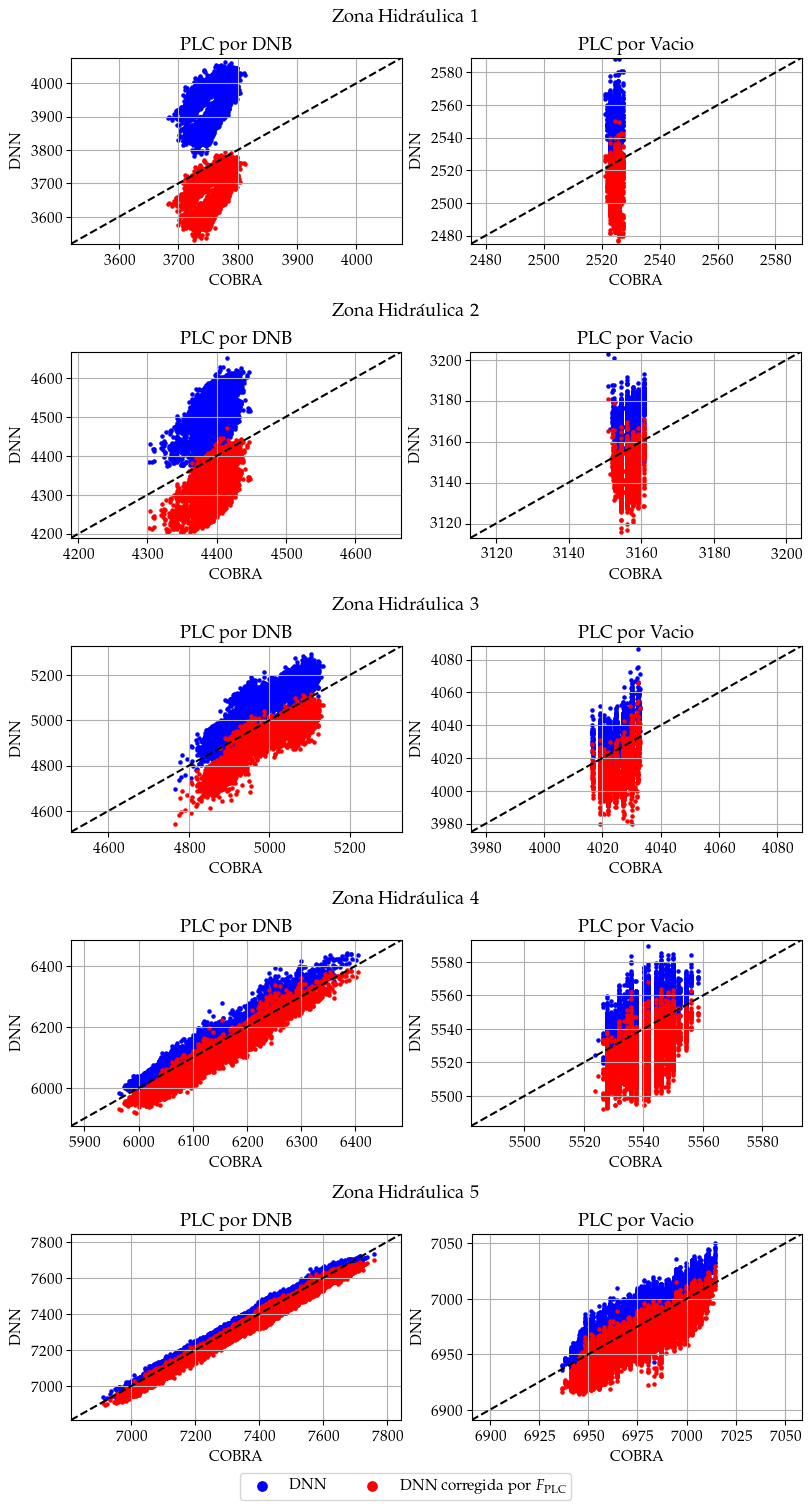
\includegraphics[width=\textwidth]{Figures/plc_pred_corr.png}
    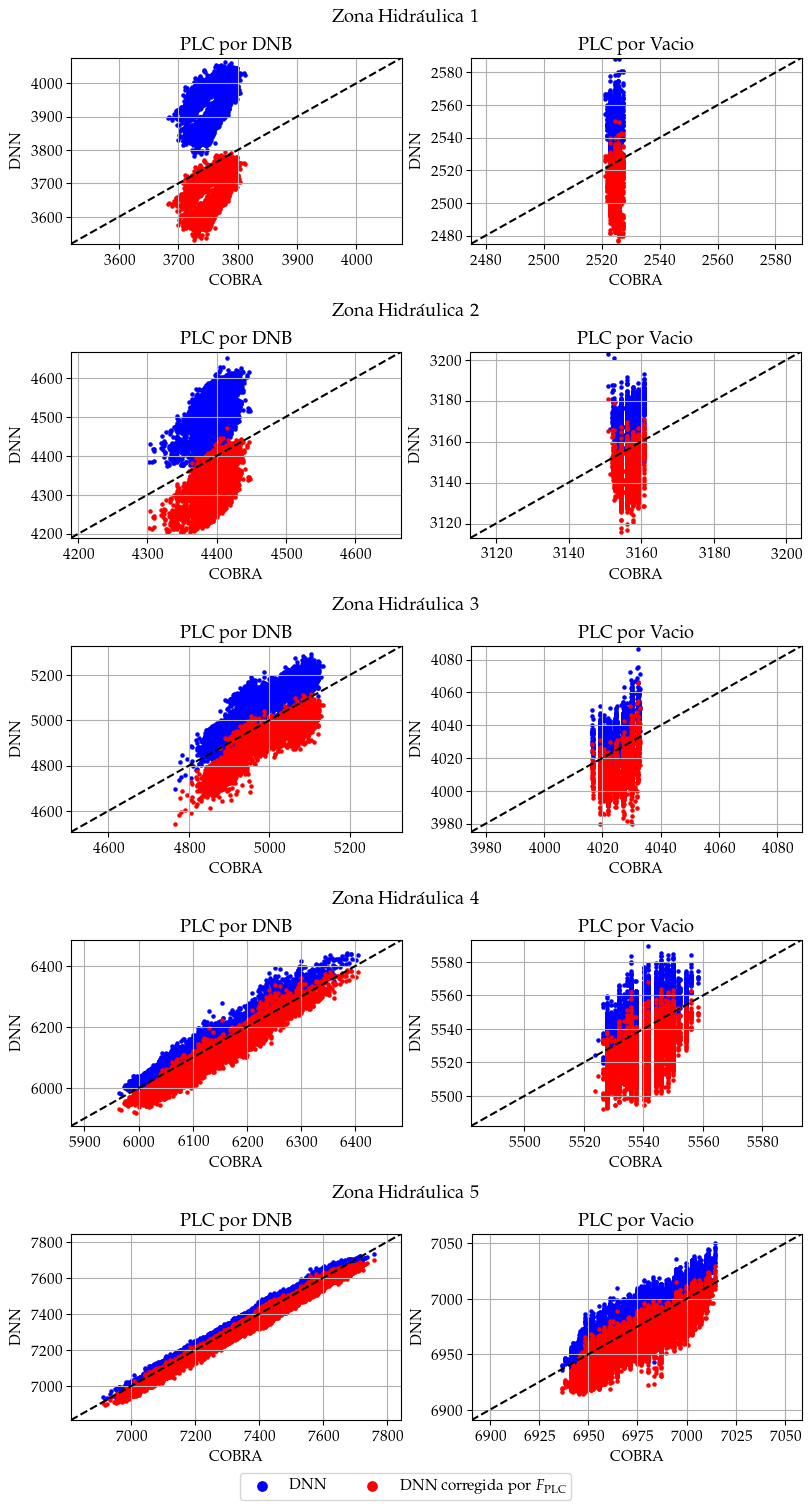
\includegraphics[height=\textheight]{Figures/plc_pred_corr.png}
    \caption{Resultados de estimación de PLC por DNBR y fracción de vacío con factor de corrección, por zona hidráulica.}
    \label{fig:plc_results_corr}
\end{figure}

\begin{table}[H]
	\centering
	\caption{Media y desvío estándar de cociente predicho-real, y factor de 95\% de probabilidad y confianza. Por zona hidráulica.}
	\begin{tabular}{c c c c c c c } 
        \toprule
        \multirow{2}{*}{\textbf{Zona Hidráulica}} & \multicolumn{3}{c}{\textbf{DNBR}} & \multicolumn{3}{c}{\textbf{Fracción de vacío}} \\
            & media & $\sigma$  & F     & media & $\sigma$  & F     \\
        1 & $1.047$ & $0.015$ & $0.933$ & $1.008$ & $0.004$ & $0.985$ \\
        2 & $1.025$ & $0.010$ & $0.961$ & $1.003$ & $0.002$ & $0.993$ \\
        3 & $1.018$ & $0.010$ & $0.967$ & $1.002$ & $0.002$ & $0.995$ \\
        4 & $1.003$ & $0.003$ & $0.991$ & $1.001$ & $0.002$ & $0.996$ \\
        5 & $1.001$ & $0.002$ & $0.995$ & $1.001$ & $0.001$ & $0.997$ \\
		\bottomrule
	\end{tabular}
	\label{tab:plc_f}
\end{table}

\begin{table}[H]
	\centering
	\caption{Tiempos de cómputo para cálculo de PLC.}
	\begin{tabular}{l l c c c c c} 
        \toprule
        & & \multicolumn{3}{c}{\textbf{Tiempo}} & \multicolumn{2}{c}{\multirow{2}{*}{\textbf{Mejora}}} \\
        & & \multirow{2}{*}{\textbf{COBRA3-CP [s]}} & \multicolumn{2}{c}{\textbf{DNN [ms]}} &  \\
        & &                                     & CPU & GPU & CPU & GPU \\
        \hline
        \multirow{4}{1.5cm}{DNBR}   
                                & mínimo        & $8.53$      & $0.28$  & $0.47$ & 3 562   & 406 \\
                                & media         & $25.16$     & $2.66$  & $3.03$ & 9 519   & 8 409\\
                                & máximo        & $137.95$    & $5.88$  & $5.51$ & 57 882 & 48 363\\
                                & \textbf{total}& 306 h     & 117 s & 130 s& 9 445  & 8 503\\
        \hline
        \multirow{4}{1.5cm}{Fracción de vacío}  
                                & mínimo        & $1.07$      & $0.21$  & $0.33$  & 432   & 405\\
                                & media         & $6.09$      & $2.46$  & $2.80$  & 2 486  & 2 197\\
                                & máximo        & $14.70$     & $5.70$  & $6.69$  & 5 955  & 5 385\\
                                & \textbf{total}& 74 h     & 108 s & 120 s & 2 479  & 2 224\\
		\bottomrule
	\end{tabular}
	\label{tab:plc_tiempos}
\end{table}

Por último, en la tabla \ref{tab:plc_margen_perdido} se observan los márgenes de potencia perdidos al aplicar la predicción de DNN. Es decir, la diferencia porcentual de potencia entre el valor de referencia y el predicho, corregido por $F_\mathrm{PLC}$. Se presentan los valores de margen medio y de margen máximo. Luego se computa el total como el promedio ponderado por la cantidad de canales que pertenecen a cada ZH.
Se obtuvieron valores decrecientes de la ZH 1 a la 5 tanto por DNBR como por fracción de vacío, a excepción de la ZH 3, que presenta el valor máximo de margen perdido por DNBR. Los valores máximos en las zonas periféricas resultan altos, aunque dentro de los porcentajes de margen tomados como criterio de seguridad al calcular una estrategia de recambio de combustibles.
Es importante tener en cuenta que las ZZHH 1 a 4 están actualmente limitadas por fracción de vacío, y la ZH 5 por DNBR. 

Finalmente, los márgenes perdidos totales medios son del $0.7$\% para DNBR y $0.5$\% para fracción de vacío. Esto expresa la capacidad del modelo de predecir con precisión y seguridad la PLC, sin un resultado demasiado conservativo. Además, debe tenerse en cuenta que las zonas periféricas operan con un importante margen, muy superior al perdido por la utilización del modelo para fracción de vacío. Por lo tanto, el margen expuesto como perdido en rigor no se pierde.

\begin{table}[H]
	\centering
	\caption{Margen perdido medio y máximo por utilizar DNN, según zona hidráulica y total.}
	\begin{tabular}{c c c c c } 
        \toprule
        \multirow{3}{*}{\textbf{Zona Hidráulica}} & \multicolumn{4}{c}{\textbf{Margen perdido [\%]}} \\ \cline{2-5}
        & \multicolumn{2}{c}{\textbf{DNBR}} & \multicolumn{2}{c}{\textbf{Fracción de vacío}} \\
          & medio & máximo & medio & máximo \\ \hline
        1 & $1.56$ & $4.56$ & $2.58$ & $5.22$ \\
        2 & $1.35$ & $4.29$ & $1.05$ & $2.28$ \\
        3 & $1.88$ & $5.37$ & $0.74$ & $1.87$ \\
        4 & $0.58$ & $2.12$ & $0.41$ & $1.25$ \\
        5 & $0.38$ & $1.37$ & $0.24$ & $0.89$ \\ \hline
        \textbf{total} & $0.71$ & $2.34$ & $0.54$ & $1.45$ \\
		\bottomrule
	\end{tabular}
	\label{tab:plc_margen_perdido}
\end{table}

\subsection{Aplicación de embeddings}
Como se explicó en la sección \ref{sec:arq_embeddings}, se aplicó una arquitectura de autoencoder para obtener el espacio latente de los perfiles de potencia axial y por barras. La arquitectura empleada fue simple, ya que esta tarea no requiere una red densa. Se optó por un encoder con 2 capas ocultas, la primera de 64 neuronas y la segunda de 32. El decoder, por su parte, es el espejo del encoder.

Se buscó el espacio latente de menor dimensión tal que la reconstrucción del vector de entrada en el conjunto de entrenamiento tuviera un coeficiente de determinación $\mathrm{R}^2>0.99$. El proceso de cálculo recorrió desde un espacio latente de dimensión 1 hasta la primera dimensión que cumpliera con la condición establecida. Para el entrenamiento se utilizó el mismo conjunto de datos que para el estimador de PLC.

Para ambos perfiles de potencia se obtuvo un espacio latente de 3 dimensiones. En la figura \ref{fig:embeddings_axial} se presentan, para cada componente del espacio latente, los 3 perfiles con mayor valor de la componente, los 3 con valores medianos y los 3 con menor valor. La primera componente puede interpretarse como el clásico factor de forma de los perfiles axiales, donde los perfiles de menor valor corresponden a la forma típicamente llamada ``panza arriba''. La segunda componente tiene un significado similar; se asocia con perfiles cuya zona inferior o superior está aplanada. Por último, la tercera componente representa potencia disminuida en el centro del perfil.

\begin{figure}[H]
    \centering
    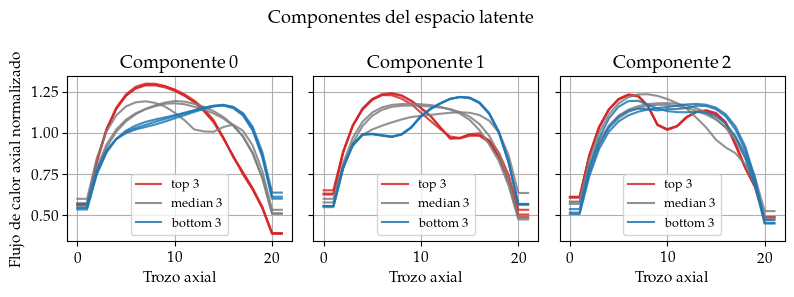
\includegraphics[width=\textwidth]{Figures/embeddings_axial_componentes_latente.png}
    \caption{Gráficos de perfiles axiales con valores más altos, medianos y bajos de cada componente del espacio latente.}
    \label{fig:embeddings_axial}
\end{figure}

En la figura \ref{fig:embeddings_radial} se presenta el gráfico análogo para el perfil por barras. En este caso, resulta más difícil obtener una explicación de cada componente.

\begin{figure}[hbtp]
    \centering
    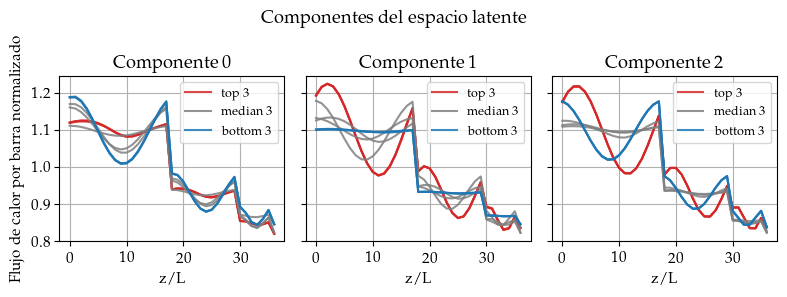
\includegraphics[width=\textwidth]{Figures/embeddings_radial_componentes_latente.png}
    \caption{Gráficos de perfiles radiales con valores más altos, medianos y bajos de cada componente del espacio latente.}
    \label{fig:embeddings_radial}
\end{figure}

Una vez entrenado el encoder, se evaluó la arquitectura del predictor de PLC, pero con el espacio latente de los perfiles de potencia como entradas. Se plantearon tres modelos, que utilizan el espacio latente del perfil axial, el del perfil por barras y ambos espacios latentes. En la tabla \ref{tab:plc_emb_errors_dnbr_vacio} se presentan la media y el desvío estándar del error con signo, para los tres modelos con embeddings y el modelo base. Los tres modelos presentan una reducción de la media del error en ambas variables objetivo. En cuanto al desvío estándar, para DNBR no se obtiene una reducción significativa, pero para fracción de vacío se reduce a aproximadamente la mitad. Es importante señalar que los modelos con embeddings del perfil por barras y de ambos perfiles presentan una media positiva del error de DNBR. Por otro lado, los tres modelos presentan un error medio negativo para la fracción de vacío. Estos dos puntos son un resultado no conservativo, aunque no de forma excesiva.

\begin{table}[h]
	\centering
	\caption{Media y desvío estándar del error con signo para cada objetivo, para modelos con embeddings.}
	\begin{tabular}{l c c c c c} 
        \toprule
        \multirow{2}{*}{\textbf{Modelo}} & \multirow{2}{*}{\textbf{Conjunto}} & \multicolumn{2}{c}{\textbf{DNBR}} & \multicolumn{2}{c}{\textbf{Fracción de vacío}} \\
        &         & media     & $\sigma$  & media & $\sigma$  \\ \hline
        \multirow{2}{*}{Base}
        & Train   &  $-0.006$    & $0.021$     & $0.018$ & $0.040$ \\
        & Test    &  $-0.006$    & $0.017$     & $0.018$ & $0.032$ \\ \hline
        \multirow{2}{*}{Emb. perfil axial}
        & Train   & $-0.002$ & $0.018$ & $-0.002$ & $0.021$ \\
        & Test    & $-0.001$ & $0.020$ & $-0.002$ & $0.022$   \\   \hline
        \multirow{2}{*}{Emb. perfil por barras}
        & Train   & $0.001$ & $0.013$ & $-0.006$ & $0.021$ \\
        & Test    & $0.001$ & $0.014$ & $-0.006$ & $0.022$ \\   \hline
        \multirow{2}{*}{Emb. ambos perfiles}
        & Train   & $0.000$ & $0.017$ & $-0.011$ & $0.016$ \\
        & Test    & $0.000$ & $0.020$ & $-0.010$ & $0.017$ \\

		\bottomrule
	\end{tabular}
	\label{tab:plc_emb_errors_dnbr_vacio}
\end{table}

En la tabla \ref{tab:plc_emb_margen_perdido} se presenta el margen perdido total para el modelo base y los tres modelos con embeddings. En cuanto al DNBR, solo el modelo con embeddings para el perfil por barras presenta una reducción del margen perdido. Para el margen perdido de fracción de vacío se obtiene una reducción en los tres modelos.

Se estima que la reducción del margen perdido en la PLC por DNBR al utilizar el espacio latente del perfil por barras proviene de la elevada dimensión de dicho perfil, en relación con la información que representa. Al reducir su dimensión, la DNN tendría mayor capacidad de centrar recursos en otras variables de entrada. 

En el caso de la PLC por fracción de vacío, es sabido que depende de la integral de la energía entregada y no de condiciones locales. Por lo tanto, variables de entrada globales como las componentes del espacio latente presentan una ventaja esperable en su predicción.

\begin{table}[H]
	\centering
	\caption{Margen perdido medio y máximo por utilizar DNN y embeddings, según zona hidráulica y total.}
	\begin{tabular}{c c c c c} 
        \toprule
        \multirow{3}{*}{\textbf{Modelo}} & \multicolumn{4}{c}{\textbf{Margen perdido [\%]}} \\ \cline{2-5}
        & \multicolumn{2}{c}{\textbf{DNBR}} & \multicolumn{2}{c}{\textbf{Fracción de vacío}} \\
          & medio & máximo & medio & máximo \\ \hline
        Base & $0.71$ & $2.34$ & $0.54$ & $1.45$ \\
        Emb. perfil axial       & $0.84$ & $3.05$ & $0.13$ & $0.39$ \\
        Emb. perfil por barras  & $0.61$ & $1.83$ & $0.15$ & $0.38$ \\
        Emb. ambos perfiles     & $0.99$ & $3.96$ & $0.10$ & $0.40$ \\
		\bottomrule
	\end{tabular}
	\label{tab:plc_emb_margen_perdido}
\end{table}

\newpage
\section{Estimación de CHF}

A continuación, se analizan los resultados para el modelo de estimación de CHF.
En primer lugar, se presenta el modelo predictor de CHF para geometría de tubo, a partir de los datos recopilados por Groeneveld \citep{GROENEVELD2007, USNRC2019NUREGKM0011}. Esto permite establecer una base sólida sobre la que los modelos de multifidelidad corrigen la estimación para un tubo de forma no lineal.

Luego, se presentan dos análisis respecto de la arquitectura del modelo. Ya que el trabajo propone una superposición de arquitecturas, se evalúa la contribución de cada cambio, con la referencia de un modelo simple y de la metodología actual. Se evalúa en primer lugar la arquitectura de multifidelidad, con la referencia de una implementación de una DNN tradicional. En segundo lugar, se evalúa la implementación de PINN a la red de multifidelidad, con la referencia de la arquitectura de multifidelidad base.

En tercer lugar, se analizan las variables de entrada al modelo, ya que su uso sin evaluación equivale a un modelo de caja negra, que no permite comprender su comportamiento ni su relación con la física del fenómeno. 
Citando a von Neumann: ``Con cuatro parámetros puedo ajustar un elefante, y con cinco puedo hacer que mueva su trompa''\footnotemark{}.
\footnotetext{Traducido de la frase original en inglés: ``With four parameters I can fit an elephant, and with five I can make him wiggle his trunk'' \citep{dyson2004meeting}.}
Tanto este análisis como los de arquitectura se realizaron con una penalización al modelo: se entrenó sobre casos de caudal alto y se evaluó sobre casos de caudal bajo.

Por último, se define el modelo final, entrenado con una división aleatoria de los datos. Se comparan los valores de \dnbrmin{} para las arquitecturas \mfdnn{} y \mfpinn{}. Luego se realiza una estimación del impacto de los valores obtenidos con un cálculo de PLC con las condiciones del diseño termohidráulico descriptas en el IFS.

\subsection{Modelo predictor de CHF en un tubo}
\label{sec:lfdnn_resultados}
Como se comentó en la sección \ref{sec:chf_arq}, se construyó un modelo de DNN para predecir el CHF en un tubo. Esta red se utiliza luego como entrada de las \mfdnn{} y \mfpinn{} entrenadas. Es importante notar que, para que los modelos de multifidelidad obtengan información relevante de la estimación en un tubo, esta debe ser confiable y tener valor físico. Por ello, la evaluación de la \texttt{LFDNN} entrenada no se restringe únicamente a estadísticos tradicionales. Para su evaluación se consideran tres categorías principales: su predicción de los ensayos en un tubo, su $\mathrm{DNBR}_\mathrm{min}$ derivado de sus predicciones sobre los ensayos de la Universidad de Columbia y la evolución del CHF predicho en función de los parámetros termohidráulicos. Este último criterio se propuso debido a que redes con arquitecturas muy densas y profundas lograban muy buenos resultados en los primeros dos criterios, pero al mirar en detalle la relación del CHF con los parámetros termohidráulicos se observaban tendencias no físicas.

Entonces, para encontrar una arquitectura óptima resultaba difícil recurrir a una estructura automatizada como Optuna. Se propuso, en cambio, analizar una serie limitada de arquitecturas, para evaluar el impacto del ancho y la profundidad de la red en los resultados. En la tabla \ref{tab:lfdnn_arqs} se presentan las arquitecturas evaluadas y sus métricas estadísticas. Se evaluó utilizar como función de activación la tangente hiperbólica y la función SiLU. Finalmente, la función SiLU fue la que demostró un comportamiento más estable.
Se observa que todos los modelos logran tanto en entrenamiento como en evaluación un $\mathrm{R}^2>0.95$ y un RMSE menor a $400\,\mathrm{kW/m^2}$. Los modelos con menos parámetros presentan una menor diferencia entre el RMSE del conjunto de entrenamiento y el de evaluación. Los dos modelos con mayor cantidad de parámetros presentan los mejores valores tanto de $\mathrm{R}^2$ como de RMSE. En vista de estos resultados, se podría considerar que el entrenamiento de todas las redes es satisfactorio.

\begin{table}[h]
	\centering
	\caption{Arquitecturas de \texttt{LFDNN} propuestas y métricas sobre conjuntos de entrenamiento y evaluación de ensayos en un tubo.}
	\begin{tabular}{c C{2cm} C{2cm} c c c c} 
        \toprule
        \multirow{2}{*}{\textbf{\#}} & \multirow{2}{=}{\textbf{Dim. capas ocultas}} & \multirow{2}{=}{\textbf{Cant. capas ocultas}} & \multicolumn{2}{c}{\textbf{Entrenamiento}} & \multicolumn{2}{c}{\textbf{Evaluación}} \\
        & & & $\mathbf{R^2}$ & \textbf{RMSE} & $\mathbf{R^2}$ & \textbf{RMSE} \\ \hline
        1 & 64  & 2 & $0.9553$ & $337.9$ & $0.9590$ & $322.0$ ($+0.8\%$) \\
        2 & 64  & 3 & $0.9657$ & $296.1$ & $0.9657$ & $294.3$ ($+4.2\%$) \\
        3 & 64  & 4 & $0.9749$ & $253.0$ & $0.9738$ & $257.3$ ($+14.2\%$) \\
        4 & 32  & 3 & $0.9503$ & $356.0$ & $0.9557$ & $334.6$ ($+0.3\%$) \\
        5 & 128 & 3 & $0.9746$ & $254.9$ & $0.9753$ & $249.9$ ($+9.6\%$) \\
		\bottomrule
	\end{tabular}
	\label{tab:lfdnn_arqs}
\end{table}
% Groeneveld  |            log CHF            |          CHF [kW/m2]          
% modelo       R2 tr   R2 te  RMSE tr  RMSE te   R2 tr   R2 te   RMSE tr   RMSE te
% ------------------------------------------------------------------------------
% 64x2        0.9608  0.9599   0.1583   0.1595  0.9553  0.9590     337.9     322.0
% 64x3        0.9683  0.9653   0.1425   0.1484  0.9657  0.9657     296.1     294.3
% 64x4        0.9778  0.9709   0.1192   0.1361  0.9749  0.9738     253.0     257.3
% 32x3        0.9600  0.9595   0.1600   0.1605  0.9503  0.9557     356.0     334.6
% 128x3       0.9754  0.9702   0.1254   0.1375  0.9746  0.9753     254.9     249.9

% mejor R2 en test (log):   64x4  (0.9709)
% mejor RMSE en test (log): 64x4  (0.1361)

% brecha train->test (RMSE en log):
%   64x2       +0.0012 (+0.8%)
%   64x3       +0.0059 (+4.2%)
%   64x4       +0.0169 (+14.2%)
%   32x3       +0.0005 (+0.3%)
%   128x3      +0.0121 (+9.6%)

En la tabla \ref{tab:lfdnn_dnbrmin} se presentan los resultados de las distintas arquitecturas al evaluar sobre el conjunto de datos de los ensayos de Columbia replicados con COBRA3-CP. Se presentan la media y el desvío estándar del $\mathrm{DNBR}$ predicho y el $\mathrm{DNBR}_\mathrm{min}$. Adicionalmente, se calcularon cuántos casos de los 146 presentaron el valor mínimo de CHF de la sección antes de los $250\,\mathrm{cm}$ y cuántos en los subcanales interiores, es decir, no periféricos. Esto se realizó debido a que se tiene conocimiento de que el CHF se presenta al final de la sección de ensayos y que, por cómo modela COBRA3-CP los subcanales, los periféricos son los más comprometidos para el CHF. Entonces, se observa que la arquitectura \#4 presenta dos ventajas: tiene la media y el desvío estándar más favorables, y además la menor cantidad de predicciones fuera de la región de salida. En cuanto a predicciones en subcanales internos, se encuentra en la mediana de los modelos evaluados. 


\begin{table}[h]
	\centering
	\caption{Arquitecturas de \texttt{LFDNN} propuestas y métricas sobre ensayos de bundle de la \cna{}.}
	\begin{tabular}{c c c c c c} 
        \toprule
        % \textbf{\#} & $\mathbf{\overline{\mathrm{DNBR}}}$ & $\mathbf{\sigma(\mathrm{DNBR})}$ &  $\mathbf{\mathrm{DNBR}_\mathrm{min}}$ & $Z_\mathrm{CHF} < 250\,\mathrm{cm}$ & $\mathrm{SCH}_\mathrm{CHF}$ interno \\
        \textbf{\#} & $\bm{\overline{\mathrm{DNBR}}}$ & $\bm{\sigma(\mathrm{DNBR})}$ &  $\bm{\mathrm{DNBR}_\mathrm{min}}$ & \textbf{Z entrada} & \textbf{SCH int.} \\ \hline
        1 & $0.651$ & $0.329$ & $1.266$ & 89 & 10 \\
        2 & $0.687$ & $0.403$ & $1.442$ & 72 & 6  \\
        3 & $0.512$ & $0.393$ & $1.248$ & 97 & 26 \\
        4 & $0.949$ & $0.266$ & $1.447$ & 31 & 16 \\
        5 & $0.864$ & $0.315$ & $1.454$ & 31 & 30\\
		\bottomrule
	\end{tabular}
	\label{tab:lfdnn_dnbrmin}
\end{table}

Luego se procedió a analizar en qué condiciones el modelo predice CHF. En la figura \ref{fig:lfdnn_chf_gx} se presentan, para el modelo \#4, los gráficos de CHF frente a flujo másico y título termodinámico. Los valores de flujo másico y título termodinámico corresponden al punto en ese ensayo en el que el modelo obtuvo el menor CHF. El resultado observado es preocupante. El modelo predice valores muy bajos de CHF para condiciones subenfriadas. Esto es algo definitivamente no físico y un resultado no deseado. El resto de los modelos presenta un comportamiento similar. 

Entonces, se propuso evaluar la generalización del modelo con el flujo másico y el título termodinámico. En la figura \ref{fig:lfdnn_chf_generalizacion} se presenta este análisis. Se filtraron los datos de entrenamiento de Groeneveld para considerar presiones y relaciones $\nicefrac{L}{D}$ similares a las del conjunto de COBRA3-CP, y luego se muestreó por fuera de los límites de flujo másico y título termodinámico. Los resultados explican fehacientemente por qué se tenía en la figura \ref{fig:lfdnn_chf_gx} una relación no física, específicamente con el título termodinámico. Los modelos no tienen en su conjunto de entrenamiento datos para condiciones subenfriadas, y su extrapolación en esa zona es hacia valores de CHF bajos. Este comportamiento requiere una corrección.

\begin{figure}[H]
    \centering
    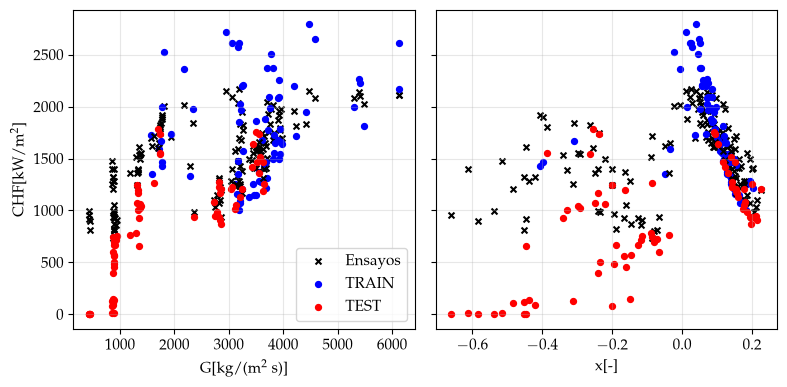
\includegraphics[width=\textwidth]{Figures/chf_lfdnn_gx_caso_mal.png}
    \caption{Relación del CHF predicho con el flujo másico y el título, según el punto predicho por el modelo \texttt{LFDNN} \#4. TRAIN y TEST son los conjuntos de entrenamiento y evaluación correspondientes a la \texttt{HFDNN}, divididos tal que en evaluación se tienen los ensayos de menor flujo másico.}
    \label{fig:lfdnn_chf_gx}
\end{figure}

Para solventar esta dificultad del modelo en la zona subenfriada se propuso una condición de monotonicidad negativa de la derivada del CHF respecto del título termodinámico, es decir, un modelo de PINN para la \lfdnn{}, que se denota \lfpinn{}. Esta incorporación se realizó al modificar el cálculo de la función de pérdida, según la ecuación \ref{eq:lfpinn_loss},
\begin{equation}
    \mathcal{L} = \mathrm{MSE}(\log \mathrm{CHF}) \;+\; \lambda \cdot \frac{1}{\sum w}\sum_i \left[w_i\,\mathrm{ReLU}\!\left(\frac{\partial \log \mathrm{CHF}}{\partial x}\Big|_i\right)\right]^2.
    \label{eq:lfpinn_loss} 
\end{equation}
Los términos $w$ y $w_i$ representan la máscara aplicada por la condición de monotonicidad sobre los puntos de colocación, según en qué región del dominio de las variables de entrada se debe aplicar. En particular, en este caso se diseñó el conjunto de puntos de colocación para la región subenfriada, con valores de presión y $\nicefrac{L}{D_h}$ en los rangos de los ensayos de COBRA3-CP. El término $\lambda$ es el peso atribuido a la condición de monotonicidad. 

\begin{figure}[h]
    \centering
    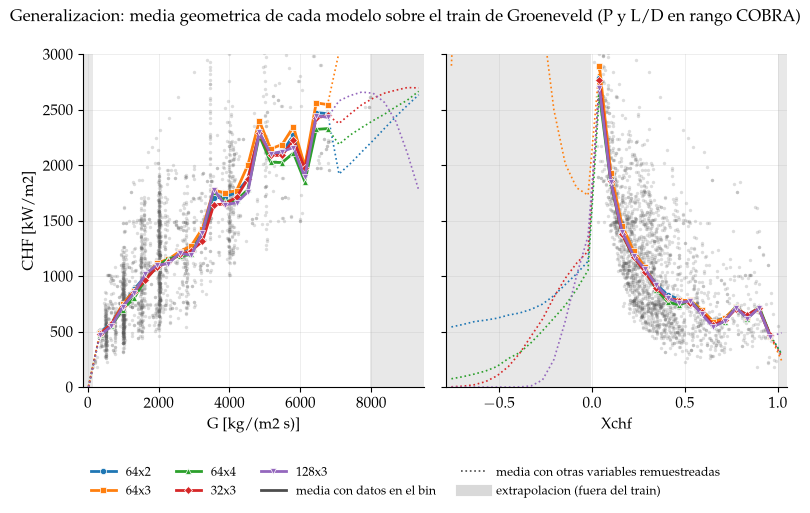
\includegraphics[width=\textwidth]{Figures/chf_lfdnn_generalizacion.png}
    \caption{Evaluación de la generalización de la \lfdnn{} respecto del flujo másico y el título termodinámico.}
    \label{fig:lfdnn_chf_generalizacion}
\end{figure}


Se analizó el impacto de esta implementación en una arquitectura de $64\times 3$, con la misma metodología que las arquitecturas anteriores. Se entrenaron tres redes, variando el valor de $\lambda$ entre $0.01$, $0.1$ y $1$. Esto permite evaluar el impacto del grado en que se impone esta condición frente a los datos.
En la tabla \ref{tab:lfdnn_arqs_comparativa} se presenta la comparativa de las métricas estadísticas sobre los conjuntos de ensayos en un tubo. Esto permite verificar que la condición agregada no perjudica al modelo dentro del conjunto que busca representar.
Se obtiene que los modelos mantienen su precisión respecto de los ensayos de un tubo. La diferencia en RMSE es de menos del $2\%$ respecto del modelo base, lo que indica que la incorporación de la monotonicidad no corrompe el modelo.

\begin{table}[h]
	\centering
	\caption{Arquitecturas de \texttt{LFDNN} propuestas y métricas sobre conjuntos de entrenamiento y evaluación de ensayos en un tubo.}
	\begin{tabular}{c c c c c c} 
        \toprule
        \multirow{2}{*}{\textbf{Arquitectura}} & \multirow{2}{*}{$\bm{\lambda}$} & \multicolumn{2}{c}{\textbf{Entrenamiento}} & \multicolumn{2}{c}{\textbf{Evaluación}} \\
        & & $\mathbf{R^2}$ & \textbf{RMSE} & $\mathbf{R^2}$ & \textbf{RMSE} \\ \hline
        Base                    & -      & $0.9657$ & $296.1$ & $0.9657$ & $294.3$ ($+4.2\%$) \\
        \multirow{3}{*}{PINN}   & $0.01$ & $0.9624$ & $310.0$ & $0.9642$ & $300.9$ ($+4.1\%$) \\
                                & $0.1$  & $0.9638$ & $304.1$ & $0.9652$ & $296.8$ ($+4.7\%$) \\
                                & $1$    & $0.9637$ & $304.6$ & $0.9650$ & $297.6$ ($+5.1\%$) \\
		\bottomrule
	\end{tabular}
	\label{tab:lfdnn_arqs_comparativa}
\end{table}

% Groeneveld                --- log CHF ---                  --- CHF [kW/m2] ---        
% modelo             R2 tr   R2 te  RMSE tr  RMSE te   R2 tr   R2 te   RMSE tr   RMSE te
% --------------------------------------------------------------------------------------
% $\lambda$ = 0     0.9665  0.9632   0.1464   0.1530  0.9605  0.9626     317.5     307.4
% $\lambda$ = 0.01  0.9661  0.9630   0.1473   0.1533  0.9624  0.9642     310.0     300.9
% $\lambda$ = 0.1   0.9661  0.9626   0.1473   0.1542  0.9638  0.9652     304.1     296.8
% $\lambda$ = 1     0.9658  0.9620   0.1479   0.1554  0.9637  0.9650     304.6     297.6

% mejor R2 en test (log):   $\lambda$ = 0  (0.9632)
% mejor RMSE en test (log): $\lambda$ = 0  (0.1530)

% brecha train->test (RMSE en log):
%   $\lambda$ = 0    +0.0066 (+4.5%)
%   $\lambda$ = 0.01 +0.0060 (+4.1%)
%   $\lambda$ = 0.1  +0.0069 (+4.7%)
%   $\lambda$ = 1    +0.0076 (+5.1%)

% costo respecto de lambda = 0 (RMSE en log, test):
%   $\lambda$ = 0    +0.00%
%   $\lambda$ = 0.01 +0.20%
%   $\lambda$ = 0.1  +0.80%
%   $\lambda$ = 1    +1.61%


Luego, en la tabla \ref{tab:lfdnn_dnbrmin_comp}, se comparan los valores de media y desvío estándar del DNBR, el $\mathrm{DNBR}_\mathrm{min}$ y los puntos predichos en la región de entrada y en subcanales interiores. Se obtiene una mejora considerable en todos los modelos PINN, lo que indica que la condición aplicada beneficia al modelo en condiciones subenfriadas. Los valores de DNBR quedan prácticamente centrados y su desvío estándar se redujo a la mitad. En cuanto al $\mathrm{DNBR}_\mathrm{min}$, no se obtuvo una mejora, pero esto se debe a su método de cálculo y a la subpredicción no física del DNBR con el modelo base. La cantidad de predicciones en la región de entrada se reduce de casi el $50\%$ de los ensayos a menos del $7\%$. En cuanto a las predicciones en subcanales internos, se obtiene un aumento, aunque se mantiene en menos de $15\%$ de los ensayos. La conclusión es que la aplicación de la monotonicidad mejora la generalización del modelo a la aplicación de interés.

\begin{table}[H]
	\centering
	\caption{Arquitecturas de \texttt{LFDNN} propuestas y métricas sobre ensayos de bundle de la \cna{}.}
	\begin{tabular}{c c c c c c c} 
        \toprule
        \textbf{Arq.} & $\bm{\lambda}$ & $\bm{\overline{\mathrm{DNBR}}}$ & $\bm{\sigma(\mathrm{DNBR})}$ &  $\bm{\mathrm{DNBR}_\mathrm{min}}$ & \textbf{Z entrada} & \textbf{SCH int.} \\ \hline
        Base    & -      & $0.687$ & $0.403$ & $1.442$ & 72 & 6  \\
        \multirow{3}{*}{PINN} 
                & $0.01$ & $1.061$ & $0.219$ & $1.470$ & 10 & 14 \\
                & $0.1$  & $1.035$ & $0.226$ & $1.457$ & 4  & 14 \\
                & $1$    & $1.037$ & $0.224$ & $1.456$ & 3  & 22 \\
		\bottomrule
	\end{tabular}
	\label{tab:lfdnn_dnbrmin_comp}
\end{table}

Se mantuvo el criterio empleado para evaluar la predicción de los modelos base y se graficó la relación del CHF predicho con el flujo másico y el título termodinámico para el modelo \lfpinn{} con $\lambda=0.1$ en la figura \ref{fig:lfdnn_chf_gx_mon}. Se observa que se predicen unos pocos casos de CHF en región subenfriada, lo que indica una mejora considerable del modelo respecto de su versión base. Adicionalmente, no se observan valores de CHF que tiendan a $0$, como en la figura \ref{fig:lfdnn_chf_gx}.
Luego, en la figura \ref{fig:lfdnn_chf_generalizacion_mono}, se presenta la evaluación de la generalización del modelo respecto del flujo másico y el título termodinámico. Se observa que el modelo ahora presenta un aumento del CHF al reducir el título termodinámico en condiciones subenfriadas. Este es el resultado esperado, reforzado por la monotonicidad aplicada. Se observa una reducción del CHF predicho en la región cercana a $x=0$, lo que se debe a los ensayos disponibles en un tubo para condiciones subenfriadas. Se halló que se tienen unos pocos ensayos de un tubo en condiciones subenfriadas, pero con longitud calefaccionada muy por debajo de las de aplicación en este trabajo. Su efecto queda compensado por la condición de monotonicidad y los puntos de colocación durante el entrenamiento. Una posible mejora a futuro es realizar un filtrado del conjunto de ensayos de Groeneveld para que las variables estén en el rango de aplicación final.

\begin{figure}[H]
    \centering
    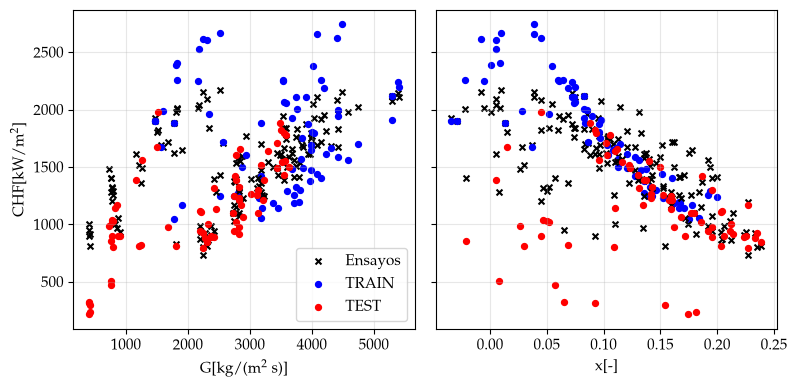
\includegraphics[width=\textwidth]{Figures/chf_lfdnn_gx_mon.png}
    \caption{Relación del CHF predicho con el flujo másico y el título, según el punto predicho por el modelo \texttt{LFDNN} con monotonicidad con $\lambda=0.1$. TRAIN y TEST son los conjuntos de entrenamiento y evaluación correspondientes a la \texttt{HFDNN}, divididos tal que en evaluación se tienen los ensayos de menor flujo másico.}
    \label{fig:lfdnn_chf_gx_mon}
\end{figure}


\begin{figure}[H]
    \centering
    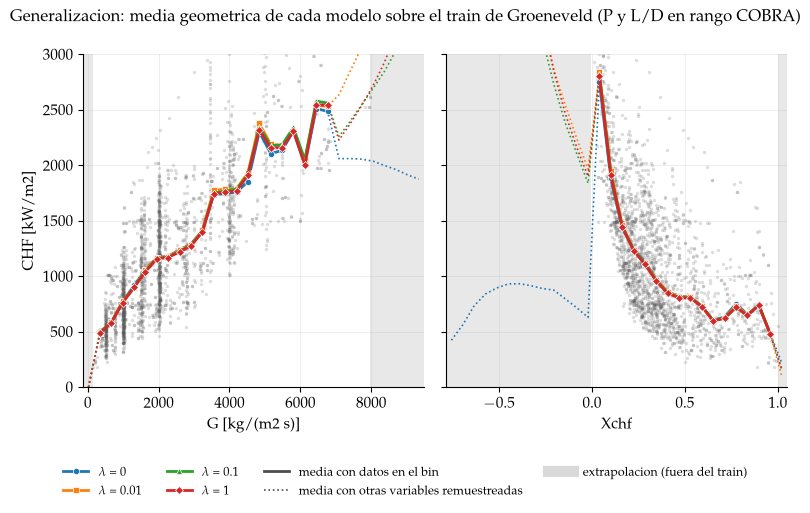
\includegraphics[width=\textwidth]{Figures/chf_lfdnn_generalizacion_mono.png}
    \caption{Evaluación de la generalización de la \lfpinn{} respecto del flujo másico y el título termodinámico, según $\lambda$.}
    \label{fig:lfdnn_chf_generalizacion_mono}
\end{figure}

Por último, en la figura \ref{fig:lfdnn_chf_pred_mono} se grafica el CHF predicho contra medido y el DNBR en cada ensayo para el modelo con $\lambda=0.1$. Se observa una predicción centrada, con algunos outliers en el conjunto de evaluación. Estos casos son los que están por fuera del rango de los ensayos en un tubo, y la red debe extrapolar para estimar CHF. A excepción de estos casos, la predicción del modelo se encuentra contenida en el mismo rango que la metodología actual propuesta por INVAP, que, además de la LUT de Groeneveld, recurre a factores de centrado y corrección desarrollados específicamente para lograr una mejor estimación del CHF en el bundle de la \cna{}, descriptos en la sección \ref{sec:app_tmf}. Esto denota que el modelo de baja fidelidad logra ya una precisión incluso comparable a la metodología actual, sin haber utilizado datos de los ensayos en la geometría específica. 

\begin{figure}[H]
    \centering
    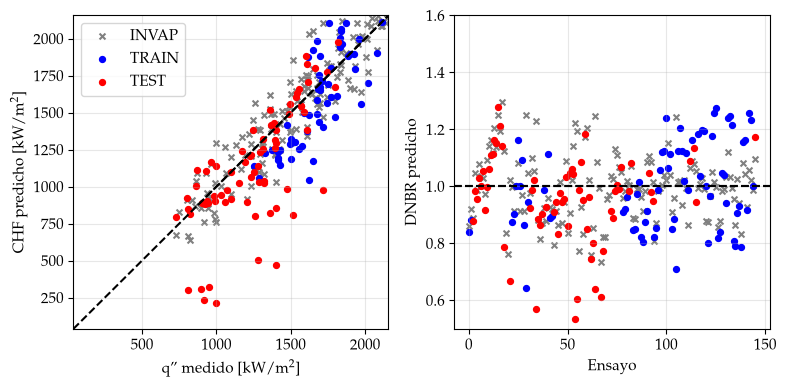
\includegraphics[width=\textwidth]{Figures/chf_lfdnn_pred_mono.png}
    \caption{Predicción de CHF contra medido y $\mathrm{DNBR}$ para cada ensayo, para modelo \lfpinn{} con $\lambda=0.1$.}
    \label{fig:lfdnn_chf_pred_mono}
\end{figure}

\newpage
\subsection{Análisis de arquitectura de multifidelidad}
\label{sec:chf_arq_mfdnn}
Para realizar el análisis de la arquitectura del modelo, se planteó separar la aplicación de multifidelidad de la de información física. En esta sección se estudió el efecto de la primera. Solo se utilizaron las variables base, tradicionales en la predicción de CHF por las LUT de Groeneveld y adoptadas por la \lfpinn{}.
Estas son el flujo másico, la presión, el título termodinámico y la relación de largo calefaccionado con diámetro hidráulico. Las primeras tres son las variables necesarias para interpolar dentro de la LUT, mientras que la cuarta permite transformar la predicción a la geometría de bundle. Groeneveld propone factores de corrección que utilizan algunas de las variables adicionales incorporadas en este trabajo. Para más detalles, ver el apéndice \ref{appendix_groeneveld}.

Las arquitecturas comparadas son las siguientes:
\begin{itemize}
    \item DNN tradicional entrenada directamente sobre las simulaciones con \break\mbox{COBRA3-CP} de los ensayos de la Universidad de Columbia. Constituye un baseline para determinar si las arquitecturas más complejas conllevan una mejora de precisión. También debe evaluarse su comportamiento en regiones no entrenadas y ponerse en tela de juicio si sus predicciones tienen sustento físico.
    % \item DNN tradicional, entrenada directamente sobre las simulaciones con \nobreak COBRA3-CP de los ensayos de la Universidad de Columbia.
    \item \lfpinn{} entrenada sobre los ensayos en un tubo utilizados para conformar las LUT 2006 de Groeneveld. Esto permite tener un baseline del aporte de la predicción de CHF en un tubo y de su contribución a la arquitectura de multifidelidad.
    \item \mfdnn{}, conjunción de la \lfpinn{} y la \hfdnn{}. Esta última fue entrenada sobre las simulaciones de COBRA3-CP de los ensayos de la Universidad de Columbia, con la predicción de la \lfpinn{} como entrada adicional.
    % \item \texttt{MFPINN}, igual a la \texttt{MFDNN}, pero con la aplicación de las relaciones físicas descriptas en la sección \ref{sec:chf_arq}.
\end{itemize}

Para lograr una evaluación que no se limitara a la capacidad de los modelos de representar la información con la que fueron entrenados, se planteó entrenarlos con los casos menos exigentes desde el punto de vista del CHF. Entonces, para dividir entre los conjuntos de entrenamiento y prueba, se utilizaron en entrenamiento aquellos ensayos con un flujo másico superior a $4\,000\,\nicefrac{\mathrm{kg}}{\mathrm{m}^2\mathrm{s}}$. La división se grafica en la figura \ref{fig:chf_div_train_test}. Además del flujo másico, la división se presenta contra el título termodinámico, donde se observa que la división también implica dejar en evaluación a la mayoría de los ensayos que presentaron CHF a título alto. Esto permite evaluar el funcionamiento del modelo al extrapolar hacia condiciones más exigentes de CHF, de forma similar a lo realizado para evaluar y definir la \lfpinn{}.

\begin{figure}[H]
    \centering
    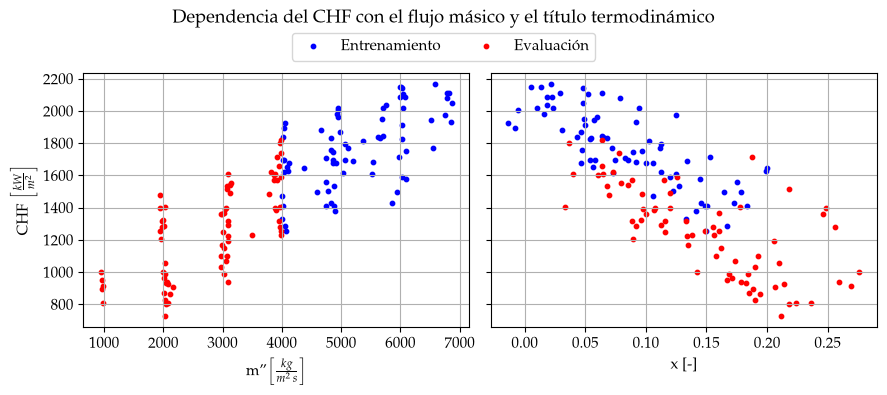
\includegraphics[width=\textwidth]{Figures/chf_division_train_test.png}
    \caption{División de los datos de CHF de la Universidad de Columbia en entrenamiento y evaluación, según flujo másico. Los ejes de flujo másico y título termodinámico corresponden a los valores promedio de la sección de ensayo a la salida.}
    \label{fig:chf_div_train_test}
\end{figure}

Para evitar que los resultados de los modelos evaluados dependan del proceso estocástico de entrenamiento, se entrenaron 50 instancias de cada modelo. De esta forma, se comparan las métricas estadísticas y de $\mathrm{DNBR}$ medias de cada modelo.
Las arquitecturas se evaluaron en su predicción de CHF de forma tradicional, y adicionalmente por medio del $\mathrm{DNBR}_\mathrm{min}$, según lo explicado en la sección \ref{sec:chf_eval}. En la tabla \ref{tab:mf_estadistica} se comparan los valores de $\mathrm{R}^2$ y de RMSE para la DNN, la \lfpinn{} y la \mfdnn{}. 
Se obtuvo un mejor rendimiento por parte de la \mfdnn{} respecto de la DNN en evaluación y muy similar en entrenamiento. En cuanto a la \lfpinn{}, su comportamiento es pobre, con un $\mathrm{R}^2<0$ que indica que una predicción constante e igual a la media obtendría un mejor ajuste.

\begin{table}[h]
	\centering
	\caption{Evaluación por métricas estadísticas de la predicción sobre el conjunto de ensayos de la Universidad de Columbia. Para DNN y \mfdnn{} representa la mediana de 50 redes entrenadas.}
	\begin{tabular}{p{2cm} l c c} 
        \toprule
        \textbf{Modelo} & \textbf{Conjunto} & $\bm{\mathrm{R}^2}$ & $\bm{\mathrm{RMSE}}$ \\ \hline
        \multirow{2}{*}{DNN}     
                & Entrenamiento & $0.951$ & $51.74$ \\
                & Evaluación    & $0.807$ & $121.59$ \\
        \multirow{2}{=}{\lfpinn{} $\lambda=0.1$}     
                & Entrenamiento & $-1.421$ & $365.39$ \\
                & Evaluación    & $-0.221$ & $305.64$ \\
        \multirow{2}{*}{\mfdnn{}}     
                & Entrenamiento & $0.945$ & $54.80$ \\
                & Evaluación    & $0.846$ & $108.67$ \\
		\bottomrule
	\end{tabular}
	\label{tab:mf_estadistica}
\end{table}

En la tabla \ref{tab:mf_dnbr} se comparan, para los mismos modelos, el factor de centrado, la media y el desvío estándar del DNBR y el $\mathrm{DNBR}_\mathrm{min}$. Es importante aclarar que el factor de centrado se calculó en función del conjunto de entrenamiento y luego se aplicó al conjunto de evaluación. De esta forma se tiene un cómputo análogo al que se realiza en inferencia. 
Se obtiene nuevamente un comportamiento similar entre el modelo DNN y \mfdnn{}, con una leve ventaja para este último en evaluación. El desvío estándar en ambos conjuntos es muy similar. En cuanto al modelo \lfpinn{}, los resultados que obtiene son peores en el conjunto de evaluación, producto de que durante su entrenamiento se expuso a menos condiciones similares. Cabe recordar que este modelo fue entrenado con otros conjuntos, correspondientes a ensayos en un tubo. Aun así, al recordar los resultados de la figura \ref{fig:lfdnn_chf_pred_mono}, su comportamiento resulta similar al de la metodología de INVAP, a excepción de entre 10 y 15 puntos en los que se subpredice el CHF.

\begin{table}[H]
	\centering
	\caption{Evaluación por métricas de predicción de $\mathrm{DNBR}$ sobre el conjunto de ensayos de la Universidad de Columbia. Para DNN y \mfdnn{} representa la mediana de 50 redes entrenadas.}
	\begin{tabular}{p{2cm} l c c c c} 
        \toprule
        \textbf{Modelo} & \textbf{Conjunto} & $\bm{f_c}$ & $\bm{\overline{\mathrm{DNBR}}}$ & $\bm{\sigma(\mathrm{DNBR})}$ & $\bm{\mathrm{DNBR}_\mathrm{min}}$ \\ \hline
        \multirow{2}{*}{DNN}     
                & Entrenamiento & \multirow{2}{*}{$1.035$}
                                        & $1.000$ & $0.031$ & $1.060$ \\
                & Evaluación    &       & $1.063$ & $0.109$ & $1.265$ \\
        \multirow{2}{=}{\lfpinn{} $\lambda=0.1$}     
                & Entrenamiento & \multirow{2}{*}{0.916}
                                        & $1.000$ & $0.152$ & $1.300$ \\
                & Evaluación    &       & $0.895$ & $0.240$ & $1.369$ \\
        \multirow{2}{*}{\mfdnn{}}     
                & Entrenamiento & \multirow{2}{*}{$1.003$}
                                        & $1.000$ & $0.032$ & $1.062$ \\
                & Evaluación    &       & $1.041$ & $0.103$ & $1.233$ \\
        % \multirow{2}{*}{MFPINN}     
        %         & Entrenamiento & \multirow{2}{*}{}
        %                                 &  &  &  \\
        %         & Evaluación    &       &  &  &  \\
		\bottomrule
	\end{tabular}
	\label{tab:mf_dnbr}
\end{table}

Al analizar el desvío estándar en el $\mathrm{DNBR}_\mathrm{min}$ obtenido en evaluación, el modelo DNN obtiene un valor de $0.088$, mientras que el \mfdnn{} $0.008$. Esto indica que este último, por su construcción, tiene una mayor robustez y no depende tanto del proceso estocástico de entrenamiento. Esto se evidencia de forma gráfica en la figura \ref{fig:chf_dnbrmin_dist}, donde se presenta la distribución de densidad de probabilidad de $\mathrm{DNBR}_\mathrm{min}$ de cada modelo, para los conjuntos de entrenamiento y de evaluación. Ambos modelos presentan buen comportamiento en entrenamiento, algo no sorprendente a esta altura del trabajo. En evaluación, los resultados permiten apreciar el impacto de tomar como entrada la predicción informada de la \lfpinn{}. El modelo de DNN tradicional presenta una distribución casi uniforme entre $1.1$ y $1.4$, mientras que el modelo \mfdnn{} presenta una distribución con menor desvío estándar y más concentrada. En particular, para esta aplicación, esto es un rasgo positivo, ya que implica que el modelo debe respetar condiciones de fondo que la aleatoriedad no puede mover, es decir, el modelo busca representar la física.

\begin{figure}[h]
    \centering
    
    % \begin{subfigure}[b]{0.60\textwidth}
    %     \centering
    %     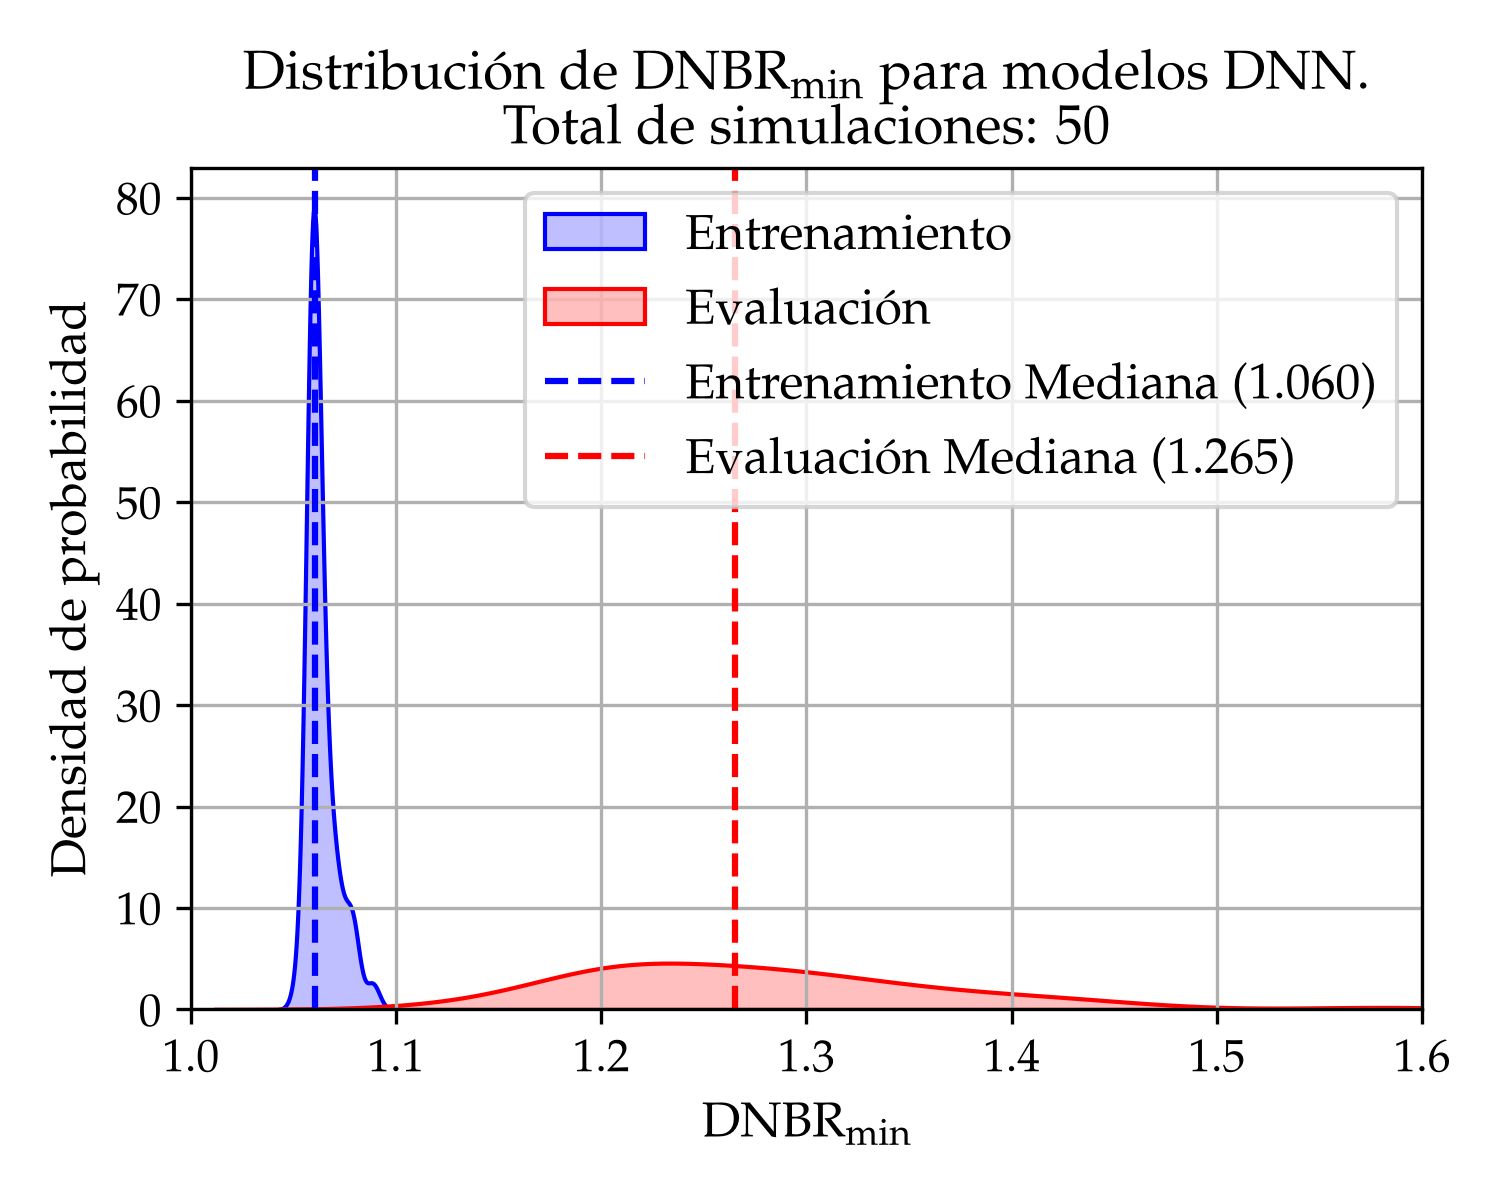
\includegraphics[width=\textwidth]{Figures/chf_distribucion_dnn.png}
    %     \caption{Modelo de DNN tradicional.}
    %     \label{fig:chf_dnbrmin_dist_dnn}
    % \end{subfigure}
    % % \hfill
    % \begin{subfigure}[b]{0.60\textwidth}
    %     \centering
    %     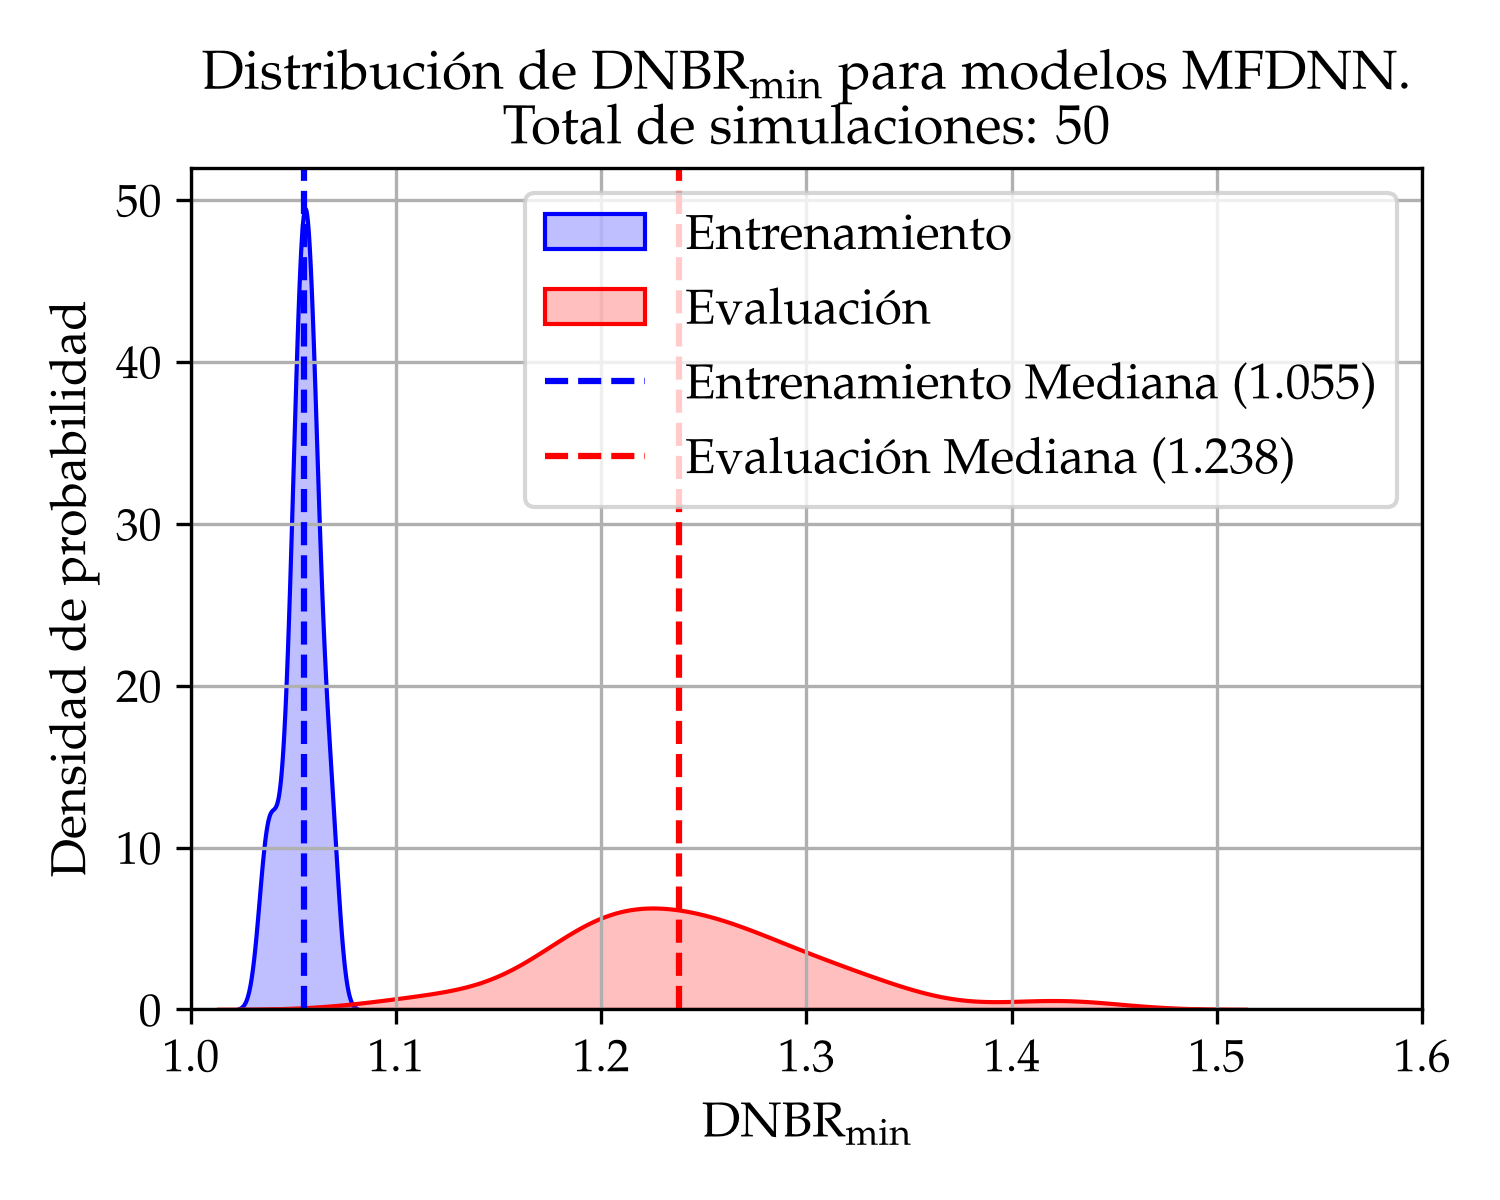
\includegraphics[width=\textwidth]{Figures/chf_distribucion_mfdnn.png}
    %     \caption{Modelo de MFDNN.}
    %     \label{fig:chf_dnbrmin_dist_mfdnn}
    % \end{subfigure}

    \begin{subfigure}[b]{0.48\textwidth}
        \centering
        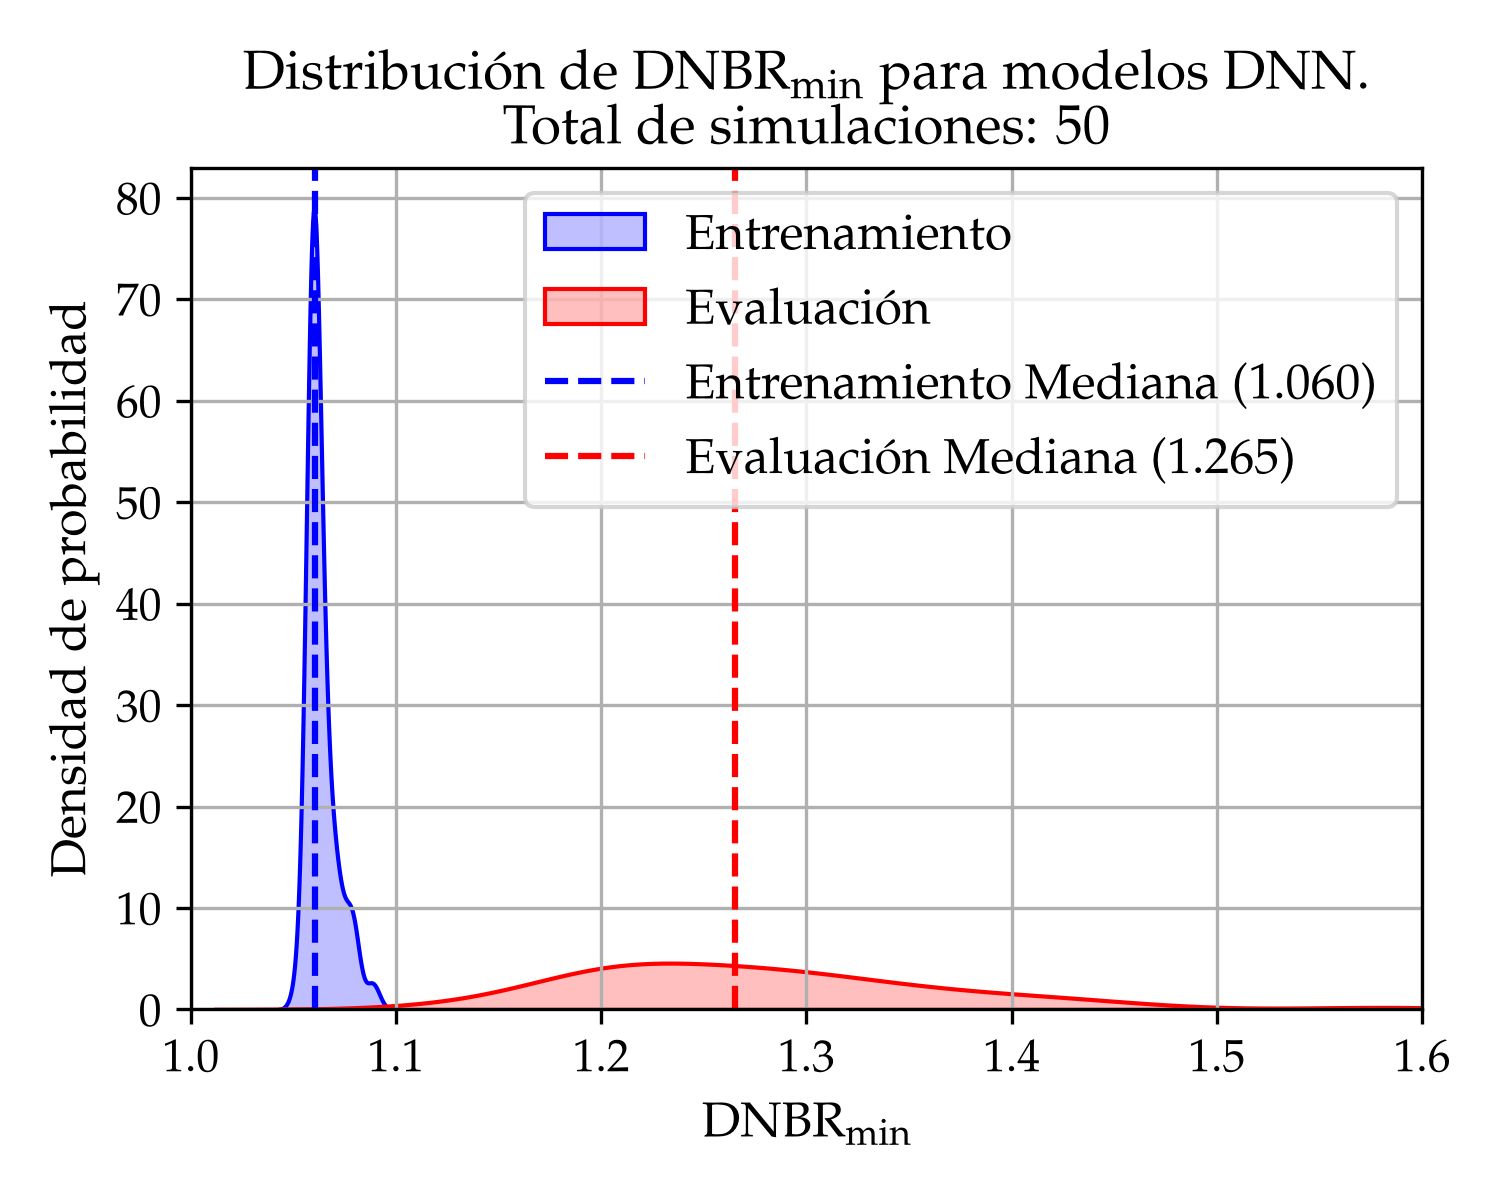
\includegraphics[width=\textwidth]{Figures/chf_distribucion_dnn.png}
        \caption{Modelo de DNN tradicional.}
        \label{fig:chf_dnbrmin_dist_dnn}
    \end{subfigure}
    \hfill
    \begin{subfigure}[b]{0.48\textwidth}
        \centering
        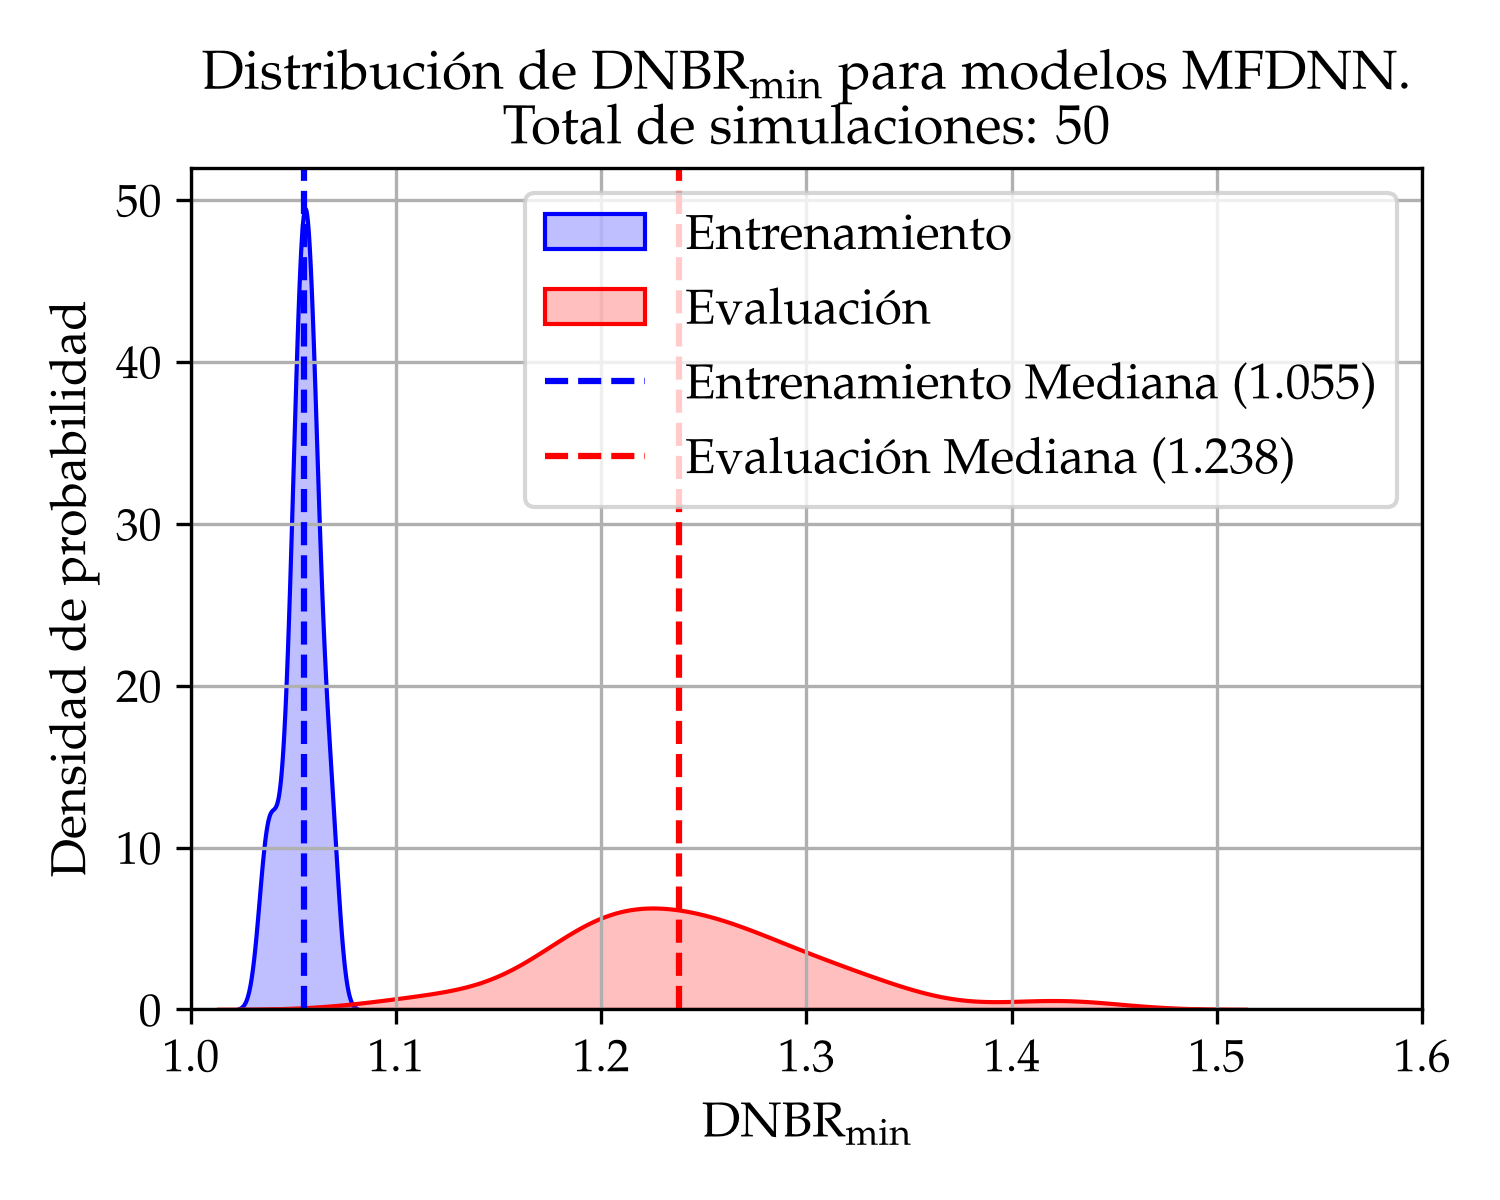
\includegraphics[width=\textwidth]{Figures/chf_distribucion_mfdnn.png}
        \caption{Modelo de MFDNN.}
        \label{fig:chf_dnbrmin_dist_mfdnn}
    \end{subfigure}
    
    \caption{Distribución de probabilidad de $\mathrm{DNBR}_\mathrm{min}$ para \mbox{$N=50$} modelos entrenados de cada tipo.}
    \label{fig:chf_dnbrmin_dist}
\end{figure}

Por último, en la figura \ref{fig:chf_pred_mfnn} se presentan los gráficos de CHF predicho contra medido y de DNBR para cada ensayo, para el modelo con la mediana del $\mathrm{DNBR}_\mathrm{min}$ de entrenamiento de cada variante. El comportamiento de ambos es similar, con una tendencia a subpredecir CHF en algunos casos del conjunto de evaluación. Aun así, se observa que, a excepción de esos puntos extraordinarios, la predicción se encuentra contenida dentro de la de INVAP. Esto indica un mejor comportamiento y destaca el rendimiento de estos modelos aun en condiciones desfavorables de entrenamiento, por no contar con los puntos más limitantes de CHF.

\begin{figure}[h]
    \centering
    
    \begin{subfigure}[b]{\textwidth}
        \centering
        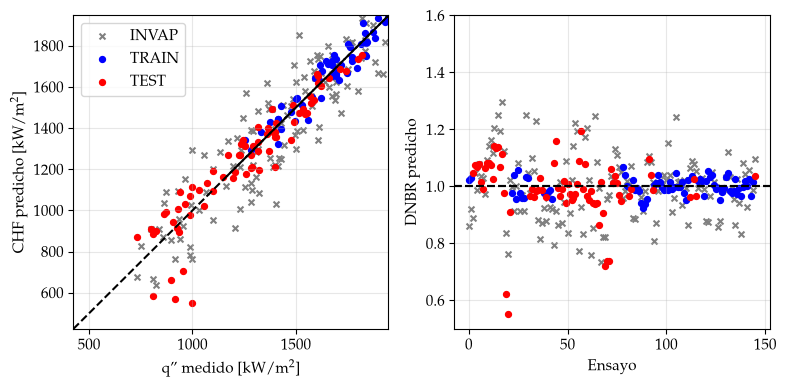
\includegraphics[width=\textwidth]{Figures/chf_dnn_pred.png}
        \caption{Modelo DNN tradicional.}
        \label{fig:chf_pred_dnn}
    \end{subfigure}
    % \hfill
    \begin{subfigure}[b]{\textwidth}
        \centering
        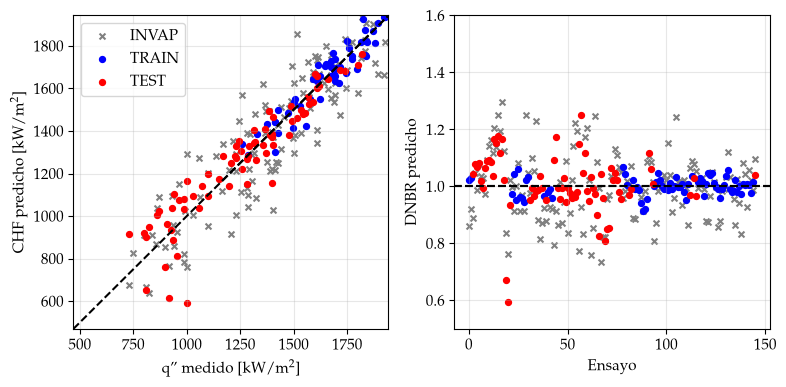
\includegraphics[width=\textwidth]{Figures/chf_mfdnn_pred.png}
        \caption{Modelo \mfdnn{}.}
        \label{fig:chf_pred_mfdnn}
    \end{subfigure}

    \caption{CHF predicho contra medido y DNBR por ensayo para modelos DNN y \mfdnn{}. Se seleccionó para cada variante el modelo con la mediana del $\mathrm{DNBR}_\mathrm{min}$ de entrenamiento.}
    \label{fig:chf_pred_mfnn}
\end{figure}

\subsection{Análisis de arquitectura informada por física}
\label{sec:chf_arq_mfpinn}
Para el análisis de arquitectura informada por física, se adoptó un enfoque de agregación de las condiciones, para poder evaluar el efecto aislado de cada una sobre el modelo. Adicionalmente, se entrenó el modelo con todas las condiciones en conjunto. En la tabla \ref{tab:mfpinn_arqs} se presenta la nomenclatura de las variantes evaluadas. Las variantes A a D fueron planteadas originalmente y, luego, en función de sus resultados, se agregó la variante E al análisis.
El punto de comparación en esta instancia es la red \mfdnn{} evaluada en la sección previa.
Para realizar la comparación se dispuso el entrenamiento de la siguiente forma. Se entrenó una red \mfdnn{} con optimizador Adam durante 500 épocas. De esta forma las redes \mfpinn{} tienen el mismo punto de partida y no dependen fuertemente del proceso estocástico detrás del optimizador para el primer acercamiento a la solución. Luego, se entrenó durante otras 500 épocas cada variante, pero con optimizador L-BFGS, estándar en entrenamiento de redes PINN.

\begin{table}[H]
	\centering
	\caption{Variantes del modelo \mfpinn{} evaluadas.}
	\begin{tabular}{c | C{1cm} | C{1cm} | C{1cm} | C{2cm} | C{2cm}} 
        \toprule
        \multirow{2}{*}{\textbf{Modelo \mfpinn{}}} & \multicolumn{3}{c|}{\textbf{Monotonicidad}} & \multirow{2}{=}{\centering \textbf{Derivada cruzada}} & \multirow{2}{=}{\centering \textbf{Derivada segunda}} \\
        & x & G & p & & \\ \hline
        A & $\blacksquare$ & $\blacksquare$ & $\blacksquare$ & $\blacksquare$ & $\blacksquare$ \\
        B & $\blacksquare$ & $\blacksquare$ & $\blacksquare$ &                &   \\
        B1& $\blacksquare$ &                &                &                &   \\
        B2&                & ${\blacksquare}^{\dagger}$ &                &                &   \\
        B3&                &                & $\blacksquare$ &                &   \\
        C &                &                &                & $\blacksquare$ &   \\
        D &                &                &                &                & $\blacksquare$ \\
        E & $\blacksquare$ & $\blacksquare$ & $\blacksquare$ &                & $\blacksquare$ \\
		\bottomrule
        \multicolumn{6}{l}{
            $\dagger$ \small{Solo se aplica la monotonicidad de G positiva en $(x<0.15)\cup(G<3\,000\,\nicefrac{\mathrm{kg}}{\mathrm{m}^2\mathrm{s}})$.}
        }
	\end{tabular}
	\label{tab:mfpinn_arqs}
\end{table}

En la tabla \ref{tab:mfpinn_arqs_dnbr_train} se compara el rendimiento de los distintos modelos en cuanto a predicción de DNBR en entrenamiento, y en la tabla \ref{tab:mfpinn_arqs_dnbr_test} en evaluación. Nuevamente, el factor de centrado fue calculado sobre el conjunto de entrenamiento y aplicado al de evaluación, de forma análoga a lo que se realiza en inferencia. Se obtiene un rendimiento idéntico entre los modelos en el conjunto de entrenamiento, con una leve mejora respecto del modelo base \mfdnn{}. Esta mejora en todos los modelos es esperable, dado que se dispuso de más épocas de entrenamiento sobre el mismo conjunto.


\begin{table}[h]
	\centering
	\caption{Resultados de predicción de CHF en conjunto de entrenamiento para las arquitecturas evaluadas de \mfpinn{}.}
	\begin{tabular}{c c c c c} 
        \toprule
        \textbf{Modelo} & $f_c$ & $\overline{\mathrm{DNBR}}$ & $\sigma(\mathrm{DNBR})$ & $\mathrm{DNBR}_\mathrm{min}$ \\ \hline
        \mfdnn{}& $1.000$
                                        & $1.000$ & $0.032$ & $1.062$ \\
        A       & $1.000$
                                        & $1.000$ & $0.019$ & $1.037$ \\
        B       & $1.000$
                                        & $1.000$ & $0.021$ & $1.041$ \\
        B1      & $1.000$
                                        & $1.000$ & $0.021$ & $1.042$ \\
        B2      & $1.000$
                                        & $1.000$ & $0.020$ & $1.040$ \\
        B3      & $1.000$
                                        & $1.000$ & $0.023$ & $1.044$ \\
        C       & $1.000$
                                        & $1.000$ & $0.019$ & $1.038$ \\
        D       & $1.000$
                                        & $1.000$ & $0.022$ & $1.044$ \\
        E       & $1.000$
                                        & $1.000$ & $0.020$ & $1.039$ \\
		\bottomrule
	\end{tabular}
	\label{tab:mfpinn_arqs_dnbr_train}
\end{table}

Luego, en evaluación, se obtienen resultados más diversos. Las variantes A, B2 y B3 logran mejorar el rendimiento de la referencia. Se obtuvo un aumento generalizado del desvío estándar y, en los modelos A a B2, una tendencia a subpredecir DNBR, mientras que en los modelos B3 a D se observó una tendencia a sobrepredecir. El modelo E, combinación de los modelos B y D, obtiene una mejora de rendimiento muy cercana a la del modelo completo A. Esta combinación se realizó no en función de los resultados de \dnbrmin{}, sino a partir de los gráficos de CHF predicho contra medido, presentados en las figuras \ref{fig:chf_pred_mfpinn_a}, \ref{fig:chf_pred_mfpinn_b} y \ref{fig:chf_pred_mfpinn_d} para las variantes A, B y D, respectivamente. 
Allí se observa el rendimiento similar entre el modelo completo A y el B, con algunos outliers adicionales en este último, que producen la reducción de rendimiento. Resulta muy interesante el modelo D en la figura \ref{fig:chf_pred_mfpinn_d}, que presenta una distribución muy cercana a la recta unitaria, con tres ensayos de sobrepredicción importante del CHF. Estos tres puntos son los que penalizan fuertemente el resultado de \dnbrmin{} de este modelo. Por este motivo se planteó la combinación de los modelos B y D en el E. Los resultados de CHF predicho contra real se presentan en la figura \ref{fig:chf_pred_mfpinn_e}, donde se observa un rendimiento sin los casos de sobrepredicción de CHF del modelo D y con una nube más cercana a la recta unitaria que el modelo B. En todos los modelos evaluados se obtuvo subpredicción de CHF para los ensayos con menor caudal. Esto se evidencia en las figuras \ref{fig:chf_gx_mfpinn_a}, \ref{fig:chf_gx_mfpinn_b} y \ref{fig:chf_gx_mfpinn_d}, donde se presentan los resultados de CHF en función del flujo másico y el título termodinámico para las variantes A, B y D, respectivamente.

En función de los resultados de esta sección, se definió utilizar la variante E como modelo final \mfpinn{}.

El máximo \dnbrmin{} para \mfdnn{} fue $XXX$ y para \mfpinn{} $XXX$.

\begin{table}[h]
	\centering
	\caption{Resultados de predicción de CHF en conjunto de evaluación para las arquitecturas evaluadas de \mfpinn{}.}
	\begin{tabular}{c c c c c} 
        \toprule
        \textbf{Modelo} & $f_c$ & $\overline{\mathrm{DNBR}}$ & $\sigma(\mathrm{DNBR})$ & $\mathrm{DNBR}_\mathrm{min}$ \\ \hline
        \mfdnn{}& $1.000$
                                        & $1.031$ & $0.094$ & $1.217$ \\
        A       & $1.000$
                                        & $0.965$ & $0.117$ & $1.196$ \\
        B       & $1.000$
                                        & $0.999$ & $0.146$ & $1.289$ \\
        B1       & $1.000$
                                        & $0.939$ & $0.171$ & $1.277$ \\
        B2       & $1.000$
                                        & $0.961$ & $0.124$ & $1.207$ \\
        B3       & $1.000$
                                        & $1.006$ & $0.103$ & $1.210$ \\
        C       & $1.000$
                                        & $1.005$ & $0.217$ & $1.436$ \\
        D       & $1.000$
                                        & $1.028$ & $0.188$ & $1.400$ \\
        E       & $1.000$
                                        & $0.961$ & $0.122$ & $1.203$ \\
		\bottomrule
	\end{tabular}
	\label{tab:mfpinn_arqs_dnbr_test}
\end{table}

\begin{figure}[H]
    \centering
    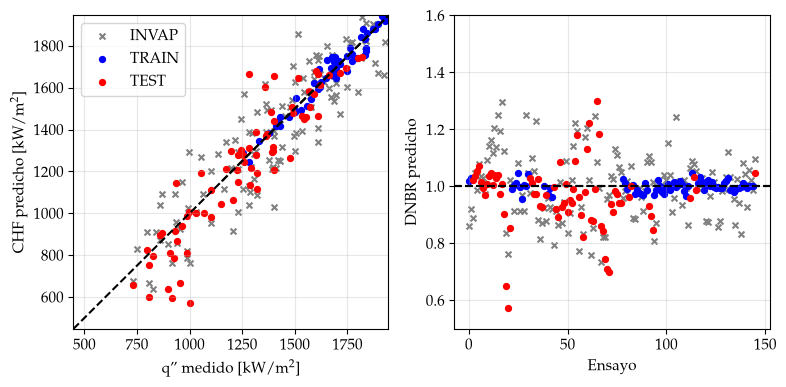
\includegraphics[width=0.95\textwidth]{Figures/chf_mfpinn_A.png}
    \caption{CHF predicho contra medido y DNBR por ensayo para variante A de \mfpinn{}.}
    \label{fig:chf_pred_mfpinn_a}
\end{figure}

\begin{figure}[H]
    \centering
    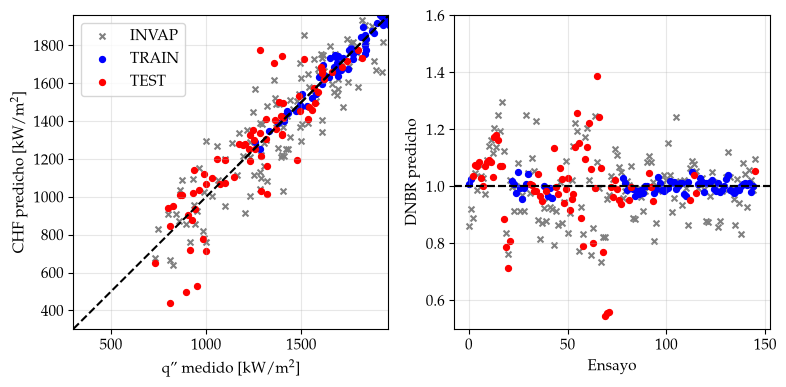
\includegraphics[width=0.95\textwidth]{Figures/chf_mfpinn_B.png}
    \caption{CHF predicho contra medido y DNBR por ensayo para variante B de \mfpinn{}.}
    \label{fig:chf_pred_mfpinn_b}
\end{figure}

\begin{figure}[H]
    \centering
    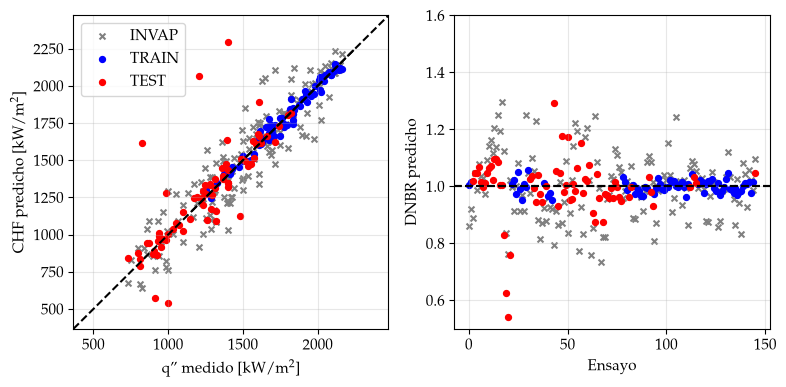
\includegraphics[width=0.95\textwidth]{Figures/chf_mfpinn_D.png}
    \caption{CHF predicho contra medido y DNBR por ensayo para variante D de \mfpinn{}.}
    \label{fig:chf_pred_mfpinn_d}
\end{figure}

% \begin{figure}[h]
%     \centering
    
%     \begin{subfigure}[b]{\textwidth}
%         \centering
%         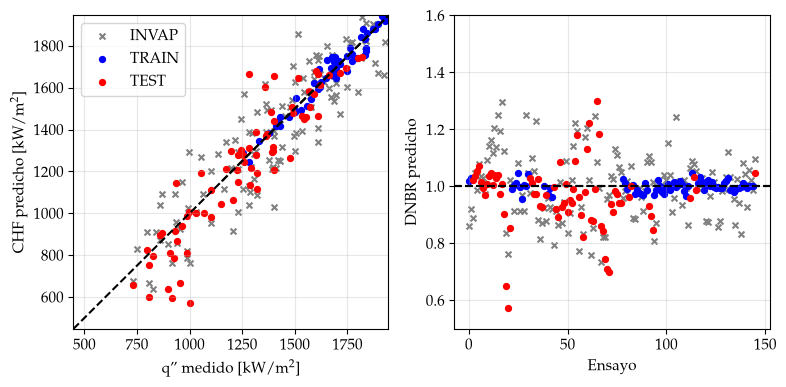
\includegraphics[width=\textwidth]{Figures/chf_mfpinn_A.png}
%         \caption{Variante A.}
%         \label{fig:chf_pred_mfpinn_a}
%     \end{subfigure}
%     % \hfill
%     \begin{subfigure}[b]{\textwidth}
%         \centering
%         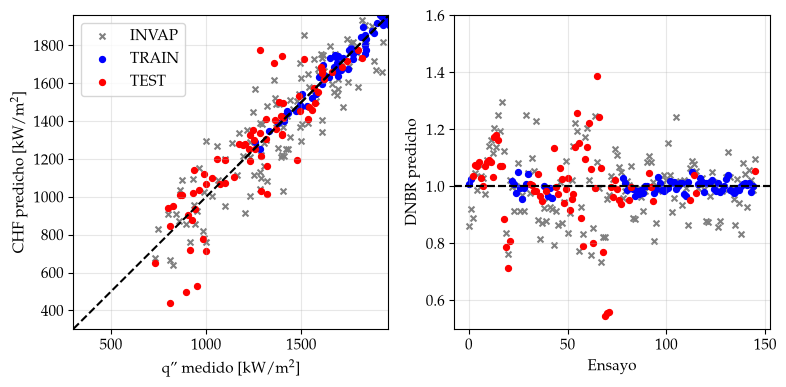
\includegraphics[width=\textwidth]{Figures/chf_mfpinn_B.png}
%         \caption{Variante B}
%         \label{fig:chf_pred_mfpinn_b}
%     \end{subfigure}

%     \begin{subfigure}[b]{\textwidth}
%         \centering
%         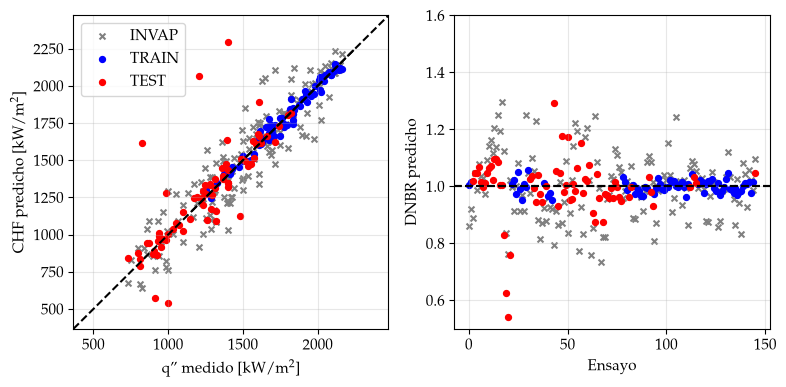
\includegraphics[width=\textwidth]{Figures/chf_mfpinn_D.png}
%         \caption{Variante D.}
%         \label{fig:chf_pred_mfpinn_d}
%     \end{subfigure}

%     \caption{CHF predicho contra medido y DNBR por ensayo para variantes A, B y D de \mfpinn{}.}
%     \label{fig:chf_pred_mfpinn_variantes}
% \end{figure}

\begin{figure}[H]
    \centering
    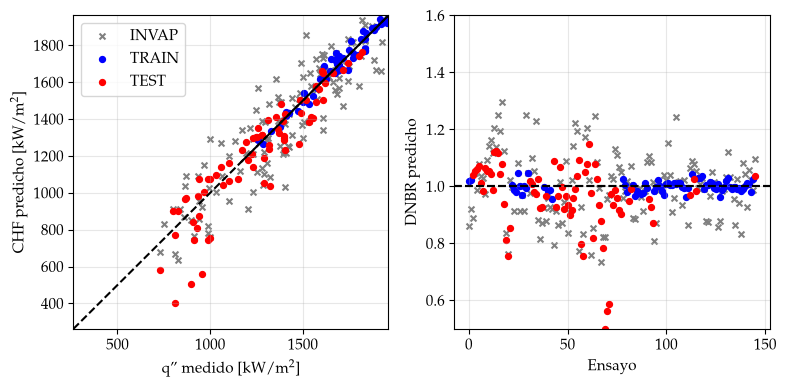
\includegraphics[width=0.95\textwidth]{Figures/chf_mfpinn_E.png}
    \caption{CHF predicho contra medido y DNBR por ensayo para variante E de \mfpinn{}.}
    \label{fig:chf_pred_mfpinn_e}
\end{figure}

% \begin{figure}[H]
%     \centering
    
%     \begin{subfigure}[b]{\textwidth}
%         \centering
%         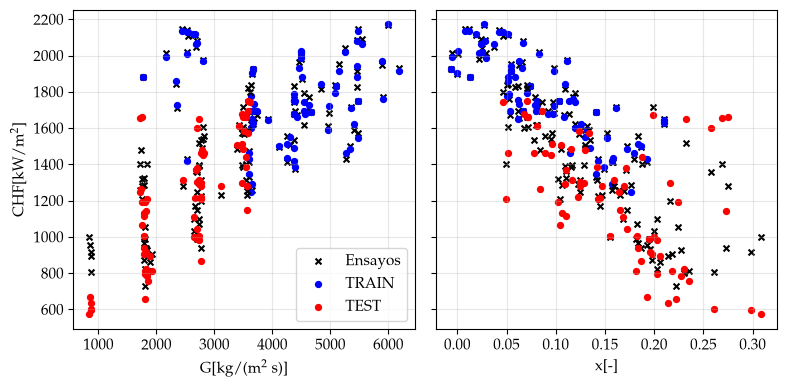
\includegraphics[width=\textwidth]{Figures/chf_mfpinn_gx_A.png}
%         \caption{Variante A.}
%         \label{fig:chf_gx_mfpinn_a}
%     \end{subfigure}
%     % \hfill
%     \begin{subfigure}[b]{\textwidth}
%         \centering
%         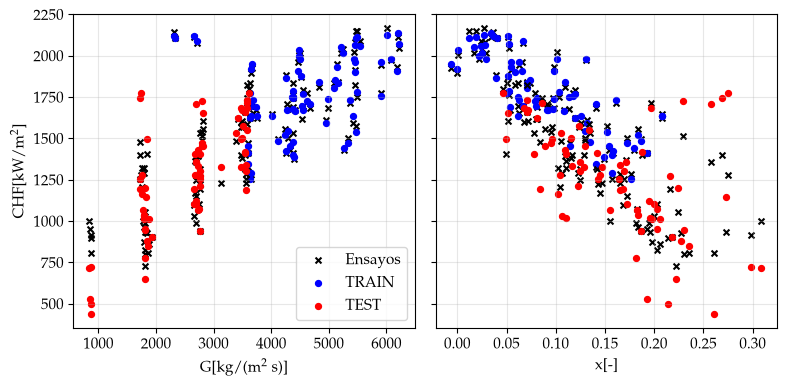
\includegraphics[width=\textwidth]{Figures/chf_mfpinn_gx_B.png}
%         \caption{Variante B}
%         \label{fig:chf_gx_mfpinn_b}
%     \end{subfigure}

%     \begin{subfigure}[b]{\textwidth}
%         \centering
%         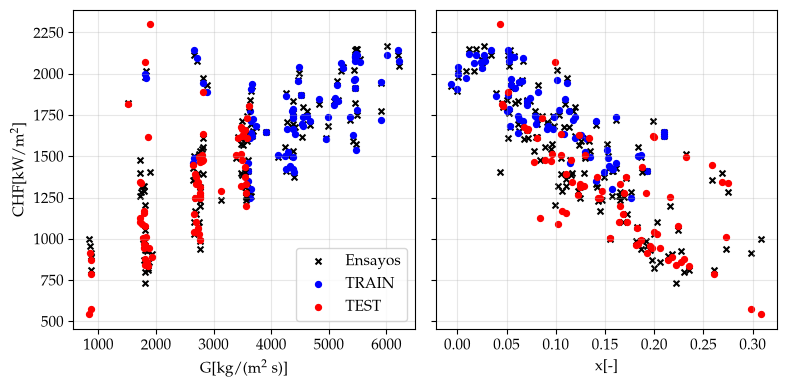
\includegraphics[width=\textwidth]{Figures/chf_mfpinn_gx_D.png}
%         \caption{Variante D.}
%         \label{fig:chf_gx_mfpinn_d}
%     \end{subfigure}

%     \caption{Relación entre CHF predicho y flujo másico y título termodinámico para variantes A, B y D de \mfpinn{}.}
%     \label{fig:chf_gx_mfpinn_variantes}
% \end{figure}

\begin{figure}[H]
    \centering
    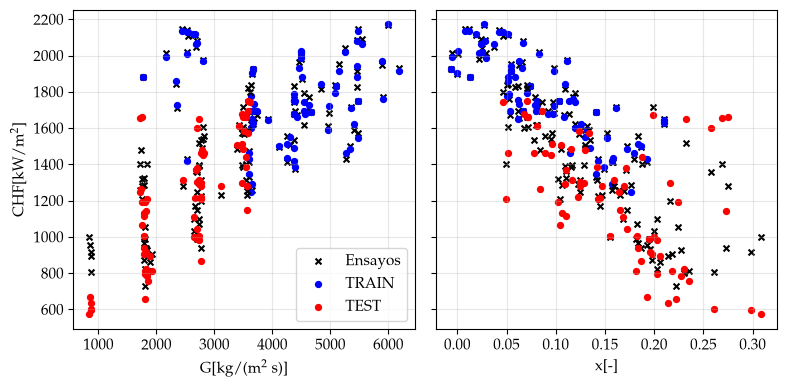
\includegraphics[width=0.95\textwidth]{Figures/chf_mfpinn_gx_A.png}
    \caption{Relación entre CHF predicho y flujo másico y título termodinámico para variante A de \mfpinn{}.}
    \label{fig:chf_gx_mfpinn_a}
\end{figure}

\begin{figure}[H]
    \centering
    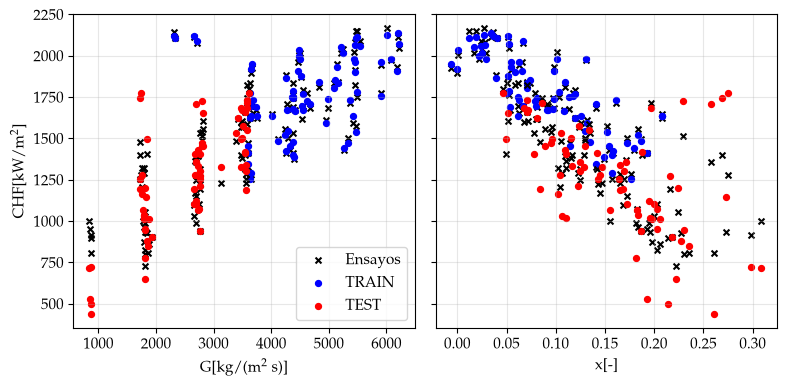
\includegraphics[width=0.95\textwidth]{Figures/chf_mfpinn_gx_B.png}
    \caption{Relación entre CHF predicho y flujo másico y título termodinámico para variante B de \mfpinn{}.}
    \label{fig:chf_gx_mfpinn_b}
\end{figure}

\begin{figure}[H]
    \centering
    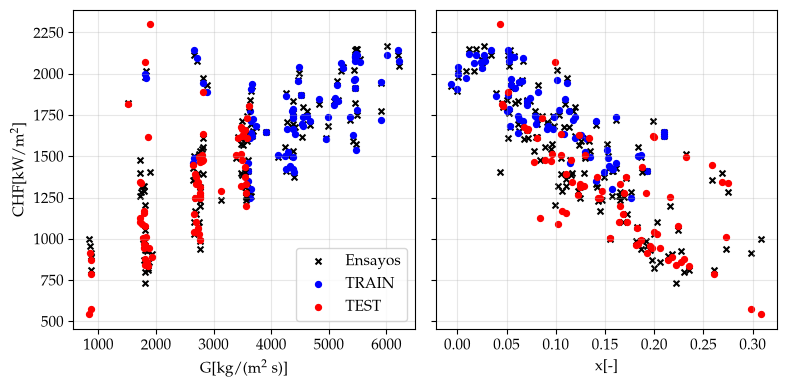
\includegraphics[width=0.95\textwidth]{Figures/chf_mfpinn_gx_D.png}
    \caption{Relación entre CHF predicho y flujo másico y título termodinámico para variante D de \mfpinn{}.}
    \label{fig:chf_gx_mfpinn_d}
\end{figure}


\subsection{Análisis de variables de entrada}
\label{sec:chf_variables_entrada}

Las variables de entrada propuestas en la sección \ref{sec:chf_pipeline} fueron el flujo másico, la presión, el título termodinámico, la relación de largo calefaccionado con diámetro hidráulico, la distancia adimensional al separador aguas arriba, el desbalance de título termodinámico respecto del valor medio del bundle, el factor de pico de potencia y la relación entre perímetro calefaccionado y mojado del subcanal. 
Las primeras cuatro variables son las clásicas utilizadas por la LUT de Groeneveld, y se consideran las más importantes para la predicción de CHF. Las cuatro variables restantes fueron propuestas en este trabajo, y se debe evaluar su contribución al modelo.

Se entrenaron el modelo \mfdnn{} y las variantes A, B, C y D del modelo \mfpinn{}. Al igual que en la sección anterior, para el modelo \mfdnn{} se entrenaron 50 instancias y se informan las medianas de las métricas. En cuanto a las variantes \mfpinn{}, no se realizó un estudio de ese tipo, debido a que su costo de entrenamiento es considerablemente elevado.

En la tabla \ref{tab:mfpinn_exp_dnbr_train} se presentan el factor de centrado, la media y el desvío estándar del DNBR predicho y el \dnbrmin{} para el conjunto de entrenamiento. Se obtuvo un rendimiento similar al del caso con las variables base, levemente mejorado en las variantes \mfpinn{}.

\begin{table}[H]
	\centering
	\caption{Resultados de predicción de CHF en conjunto de entrenamiento para las arquitecturas evaluadas de \mfpinn{}.}
	\begin{tabular}{c c c c c} 
        \toprule
        \textbf{Modelo} & $f_c$ & $\overline{\mathrm{DNBR}}$ & $\sigma(\mathrm{DNBR})$ & $\mathrm{DNBR}_\mathrm{min}$ \\ \hline
        \mfdnn{}    & $1.007$ & $1.000$ & $0.028$ & $1.055$ \\
        \mfpinn{} A & $1.000$ & $1.000$ & $0.010$ & $1.020$ \\
        \mfpinn{} B & $1.000$ & $1.000$ & $0.014$ & $1.028$ \\
        \mfpinn{} D & $1.000$ & $1.000$ & $0.018$ & $1.035$ \\
        \mfpinn{} E & $1.000$ & $1.000$ & $0.013$ & $1.026$ \\
		\bottomrule
	\end{tabular}
	\label{tab:mfpinn_exp_dnbr_train}
\end{table}

En cuanto al conjunto de evaluación, sí se obtuvieron diferencias en el rendimiento respecto de utilizar las variables base. En la tabla \ref{tab:mfpinn_exp_dnbr_test} se presentan las métricas para dicho conjunto. La \mfdnn{} presenta un rendimiento casi idéntico al caso anterior. Las variantes A y E de \mfpinn{} presentaron un rendimiento muy pobre, con un \dnbrmin{} mayor incluso que el de la \lfdnn{}. La variante B presenta una mejora, producto de una reducción del desvío estándar y un aumento en la subpredicción del CHF. 
La variante D presenta un rendimiento sobresaliente, con el mejor \dnbrmin{} obtenido hasta este punto del trabajo. Por ello, se investigó el resultado con mayor detalle, al graficar la relación de los CHF predichos con el flujo másico y el título termodinámico en la figura \ref{fig:chf_mfpinn_d_gx_exp}. Allí se puede ver que el modelo predice CHF en condiciones subenfriadas en múltiples ensayos. Este resultado pone en tela de juicio el sentido físico de estas predicciones.

\begin{table}[H]
	\centering
	\caption{Resultados de predicción de CHF en conjunto de evaluación para las arquitecturas evaluadas de \mfpinn{}.}
	\begin{tabular}{c c c c c} 
        \toprule
        \textbf{Modelo} & $f_c$ & $\overline{\mathrm{DNBR}}$ & $\sigma(\mathrm{DNBR})$ & $\mathrm{DNBR}_\mathrm{min}$ \\ \hline
        \mfdnn{}    & $1.007$ & $1.046$ & $0.097$ & $1.238$ \\
        \mfpinn{} A & $1.000$ & $1.233$ & $0.451$ & $2.125$ \\
        \mfpinn{} B & $1.000$ & $0.953$ & $0.126$ & $1.202$  \\
        \mfpinn{} D & $1.000$ & $0.956$ & $0.089$ & $1.133$  \\
        \mfpinn{} E & $1.000$ & $1.321$ & $0.358$ & $2.030$  \\
		\bottomrule
	\end{tabular}
	\label{tab:mfpinn_exp_dnbr_test}
\end{table}

\begin{figure}[H]
    \centering
    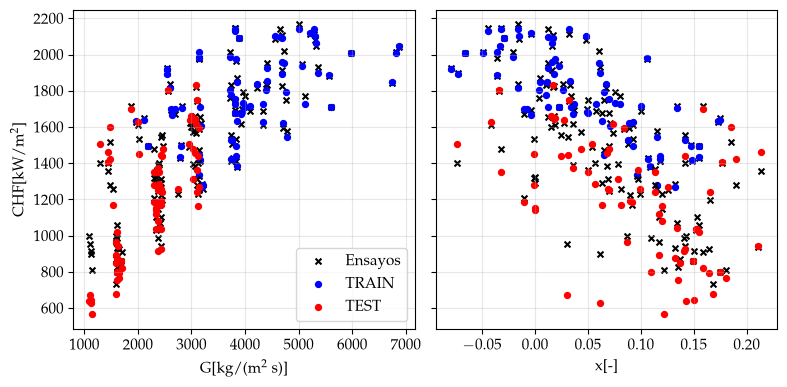
\includegraphics[width=0.95\textwidth]{Figures/chf_mfpinn_gx_D_exp.png}
    \caption{Relación de CHF con el flujo másico y el título termodinámico para variante D de \mfpinn{}, con variables de entrada expandidas.}
    \label{fig:chf_mfpinn_d_gx_exp}
\end{figure}

Se presentan los resultados de CHF predicho contra real y DNBR por ensayo para el modelo \mfdnn{} en la figura \ref{fig:chf_mfdnn_exp} y para la variante E del modelo \mfpinn{} en la figura \ref{fig:chf_mfpinn_exp}. Ambos obtienen una tendencia a la sobrepredicción para el conjunto de evaluación. Para la variante E se observa un rendimiento muy pobre, como lo indican las métricas de DNBR, con una sobrepredicción preocupante del CHF.

\begin{figure}[H]
    \centering
    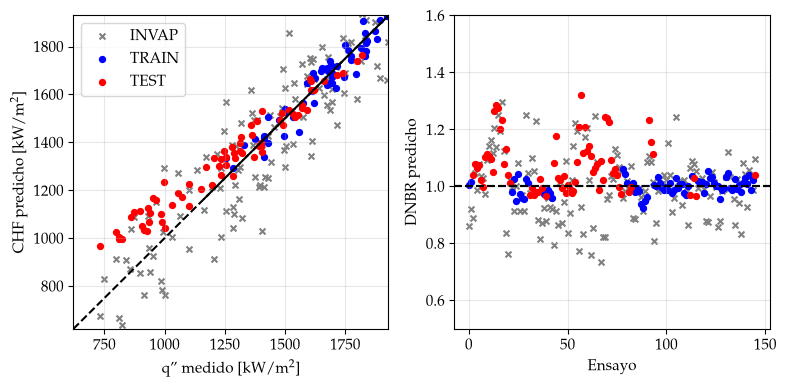
\includegraphics[width=0.95\textwidth]{Figures/chf_mfdnn_pred_exp.png}
    \caption{CHF predicho contra real y DNBR por ensayo, para \mfdnn{} con variables de entrada expandidas.}
    \label{fig:chf_mfdnn_exp}
\end{figure}

\begin{figure}[H]
    \centering
    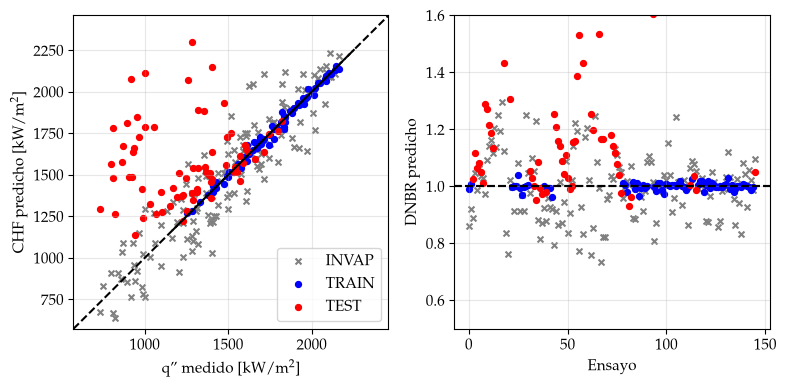
\includegraphics[width=0.95\textwidth]{Figures/chf_mfpinn_E_exp.png}
    \caption{CHF predicho contra real y DNBR por ensayo, para variante E de \mfpinn{} con variables de entrada expandidas.}
    \label{fig:chf_mfpinn_exp}
\end{figure}

La conclusión obtenida es que la inclusión de estas variables en el modelo no representa una mejora clara en las predicciones, e incluso puede resultar en predicciones con tendencias no físicas. Por lo tanto, los modelos finales solo utilizan las variables básicas.


\subsection{Modelos finales}
En las secciones \ref{sec:chf_arq_mfdnn} y \ref{sec:chf_arq_mfpinn} se validó la robustez de los modelos \mfdnn{} y \mfpinn{} para la estimación de CHF al restringir su entrenamiento a condiciones de medio a alto caudal y evaluación a bajo caudal. Dichas condiciones implican una penalización importante al modelo, ya que su conjunto de entrenamiento no contiene datos de las condiciones más críticas para el CHF. Si bien este análisis permitió validar el funcionamiento de los modelos, sus versiones finales no deben tener aplicada esta penalización. Por lo tanto, fueron entrenados con una división aleatoria entre conjuntos de entrenamiento y evaluación, con un 20\% de los datos reservados para evaluación. Se realizó la división con estratificación por conjunto de ensayos de la Universidad de Columbia, de forma de tener datos de los 4 conjuntos de ensayos disponibles.

En la tabla \ref{tab:mf_final_dnbr} se presentan los resultados de las métricas de predicción de $\mathrm{DNBR}$ para \mfdnn{} y \mfpinn{}. Adicionalmente se tienen los valores de la metodología actual, implementada por INVAP. Aquí se puede comparar directamente con ella, ya que los modelos \mfdnn{} y \mfpinn{} fueron entrenados con todo el rango de los ensayos. La metodología actual fue calibrada sin dejar un conjunto de evaluación, por lo que su capacidad de extrapolar por fuera del rango de calibración no ha sido estudiada.

El modelo \mfdnn{} obtiene un rendimiento similar a los análisis previos en el conjunto de entrenamiento, pero en este caso el \dnbrmin{} para evaluación es del mismo orden. La reducción del \dnbrmin{} es considerable respecto de la metodología actual. El modelo \mfpinn{} tiene aún mejor comportamiento, con un \dnbrmin{} en evaluación incluso menor que el de \mfdnn{} en entrenamiento. Adicionalmente, el desvío estándar también se ve reducido para el modelo \mfpinn{}, lo que indica que predice con un error consistentemente bajo.

\begin{table}[H]
	\centering
	\caption{Evaluación por métricas de predicción de $\mathrm{DNBR}$ sobre el conjunto de ensayos de la Universidad de Columbia. Para \mfdnn{} representa la mediana de 50 redes entrenadas. Entrenamiento y evaluación divididos de forma aleatoria.}
	\begin{tabular}{p{2cm} l c c c c} 
        \toprule
        \textbf{Modelo} & \textbf{Conjunto} & $\bm{f_c}$ & $\bm{\overline{\mathrm{DNBR}}}$ & $\bm{\sigma(\mathrm{DNBR})}$ & $\bm{\mathrm{DNBR}_\mathrm{min}}$ \\ \hline
        INVAP   & -           & $1.164$ & $0.999$ & $0.113$ & $1.212$ \\
        \multirow{2}{*}{\mfdnn{}}     
                & Entrenamiento & \multirow{2}{*}{$1.002$}
                                        & $1.000$ & $0.050$ & $1.094$ \\
                & Evaluación    &       & $0.998$ & $0.054$ & $1.113$ \\
        \multirow{2}{*}{\mfpinn{}}     
                & Entrenamiento & \multirow{2}{*}{$1.005$}
                                        & $1.000$ & $0.029$ & $1.056$ \\
                & Evaluación    &       & $0.987$ & $0.044$ & $1.084$ \\
		\bottomrule
	\end{tabular}
	\label{tab:mf_final_dnbr}
\end{table}

En la figura \ref{fig:dist_mfdnn_final} se presenta la distribución de densidad de probabilidad de \dnbrmin{} para los 50 modelos \mfdnn{} entrenados. Nuevamente, se evidencia un rendimiento en evaluación consistente y cercano al de entrenamiento. En la figura \ref{fig:chf_mfdnn_final} se presentan los gráficos de CHF predicho contra real y DNBR por ensayo para el modelo \mfdnn{} con el valor mediano de \dnbrmin{}. Comparado con las predicciones por la metodología INVAP, se obtiene una distribución más centrada en la recta de identidad, y todos los valores de DNBR quedan contenidos aproximadamente entre $0.9$ y $1.1$.

Finalmente, en la figura \ref{fig:chf_mfpinn_final} se presentan para el modelo \mfpinn{} los gráficos de CHF predicho contra real y de DNBR por ensayo. La distribución de predicciones es aún más cercana que la de la \mfdnn{}, lo que refuerza los valores de \dnbrmin{} presentados previamente.

\begin{figure}[H]
    \centering
    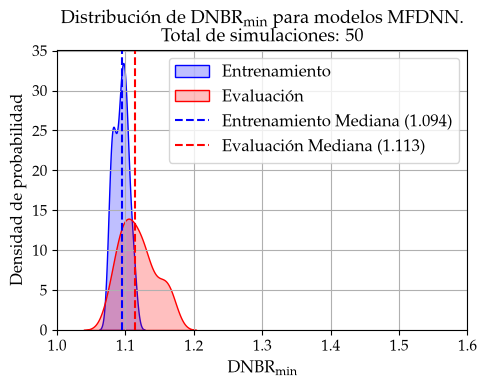
\includegraphics[width=0.6\textwidth]{Figures/chf_distribucion_mfdnn_final.png}
    \caption{Distribución de densidad de probabilidad de \dnbrmin{} para 50 modelos \mfdnn{} entrenados.}
    \label{fig:dist_mfdnn_final}
\end{figure}

\begin{figure}[H]
    \centering
    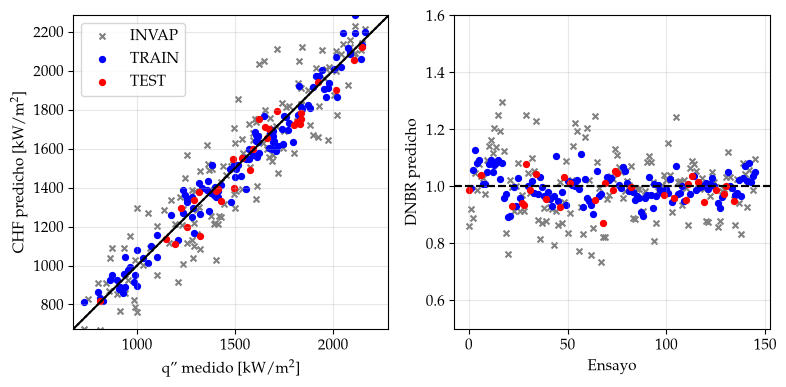
\includegraphics[width=0.95\textwidth]{Figures/chf_mfdnn_pred_final.png}
    \caption{CHF predicho contra real y DNBR por ensayo para modelo final \mfdnn{}.}
    \label{fig:chf_mfdnn_final}
\end{figure}

\begin{figure}[H]
    \centering
    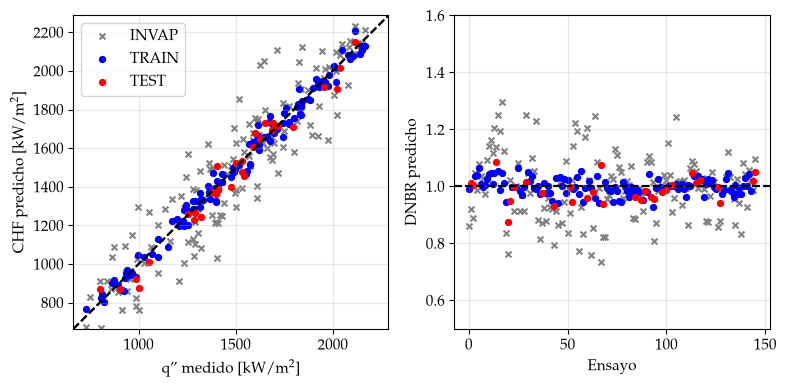
\includegraphics[width=0.95\textwidth]{Figures/chf_mfpinn_pred_final.png}
    \caption{CHF predicho contra real y DNBR por ensayo para modelo final \mfpinn{}.}
    \label{fig:chf_mfpinn_final}
\end{figure}

\subsection{Estimación de impacto}
Para estimar el impacto de la reducción del valor del \dnbrmin{} en las PLC, se utiliza el valor obtenido en evaluación de la \mfpinn{} para calcular el $\mathrm{DNBR}_\mathrm{lim}$. Luego se calcula con COBRA3-CP el valor de PLC por DNB, con los perfiles de potencia de diseño termohidráulico del IFS.
Es importante notar que esta estimación es de primer orden, puesto que el valor final del $\mathrm{DNBR}_\mathrm{lim}$ depende del límite de diseño seguro (SDL). Este límite varía por la metodología de predicción de CHF y su dependencia ante variaciones en las condiciones operativas. A priori, una predicción más robusta de CHF debería permitir reducir el $\Delta \mathrm{DNBR}_\mathrm{SDL}$, pero esa evaluación se encuentra por fuera del alcance de este trabajo ya que implica realizar todos los cálculos del diseño termohidráulico de la \cna{}.

\begin{table}[H]
	\centering
	\caption{Potencia límite de canal [MW] por DNB para metodología actual y \mfpinn{}.}
	\begin{tabular}{c c c c c c} 
        \toprule
        \multirow{2}{*}{\textbf{Metodología}} & \multicolumn{5}{c}{\textbf{Zona Hidráulica}} \\
                    & 1         & 2         & 3         & 4         & 5         \\ \hline
        Actual      & $3\,652$  & $4\,074$  & $4\,495$  & $5\,768$  & $6\,920$  \\
        \mfpinn{}   & $3\,746$  & $4\,383$  & $4\,932$  & $5\,977$  & $7\,128$  \\
        Diferencia  & $+2.6\%$  & $+7.59\%$ & $+9.72\%$ & $+3.62\%$ & $+3.01\%$ \\
		\bottomrule
	\end{tabular}
	\label{tab:mfpinn_arqs_dnbr}
\end{table}

% Chapter Template

\chapter{Conclusiones} % Main chapter title

\label{Chapter5} % Change X to a consecutive number; for referencing this chapter elsewhere, use \ref{ChapterX}
A continuación, se presentan las conclusiones del trabajo y las tareas disponibles a futuro para continuarlo.



\section{Conclusiones generales}

% La idea de esta sección es resaltar cuáles son los principales aportes del trabajo realizado y cómo se podría continuar. Debe ser especialmente breve y concisa. Es buena idea usar un listado para enumerar los logros obtenidos.

% En esta sección no se deben incluir ni tablas ni gráficos.

% Algunas preguntas que pueden servir para completar este capítulo:

% \begin{itemize}
% \item ¿Cuál es el grado de cumplimiento de los requerimientos?
% \item ¿Cuán fielmente se puedo seguir la planificación original (cronograma incluido)?
% \item ¿Se manifestó algunos de los riesgos identificados en la planificación? ¿Fue efectivo el plan de mitigación? ¿Se debió aplicar alguna otra acción no contemplada previamente?
% \item Si se debieron hacer modificaciones a lo planificado ¿Cuáles fueron las causas y los efectos?
% \item ¿Qué técnicas resultaron útiles para el desarrollo del proyecto y cuáles no tanto?
% \end{itemize}

En esta sección, se exponen las conclusiones generales de los modelos desarrollados en el trabajo.

\subsection{Estimación de PLC}
Se propuso un modelo de aprendizaje profundo para la estimación del DNBR y la fracción de vacío en un canal refrigerante de la \cna{}. El modelo tiene como entradas los parámetros termohidráulicos del canal y los perfiles de potencia axial y por barra. Se optimizaron sus hiperparámetros y se obtuvo el modelo final, con errores relativos menores al $1\%$. 

Se desarrolló un lazo de cálculo análogo al utilizado con COBRA3-CP para la estimación de PLC con el modelo desarrollado. Se comparó con cálculos de PLC realizados sobre 100 casos de la vigente estrategia de recambio de combustibles de la \cna{}. Se obtuvieron cocientes entre valor predicho y real con media menor a $1.05$. 

Para asegurar la estimación conservativa de la PLC, se propuso un factor multiplicativo de ajuste. Al utilizar este factor, se obtuvieron los márgenes perdidos por el uso de la herramienta con inteligencia artificial frente al uso de COBRA3-CP. El margen medio perdido total en el reactor es de $0.71\%$, mientras que el máximo es $2.34\%$. 

El tiempo de cómputo de la metodología propuesta fue varios órdenes de magnitud menor que el de la predicción con COBRA3-CP. En términos cuantitativos, la aplicación de esta metodología representa una mejora en el tiempo de cómputo de aproximadamente $2\,000$ veces por fracción de vacío y $8\,500$ veces por DNB.

Finalmente, se aplicó una arquitectura autoencoder para obtener el espacio latente de los perfiles de potencia axial y por barra. Los espacios latentes obtenidos permiten identificar las cualidades principales de los perfiles. Adicionalmente, se aplicó la reducción de dimensionalidad de los perfiles para modificar el vector de entrada a la DNN estimadora de DNBR y fracción de vacío. Se obtuvo una reducción del margen perdido en el caso de utilizar el espacio latente del perfil por barra, lo que demuestra que las 37 componentes son altamente redundantes para este cálculo.


\subsection{Estimación de CHF}
Se propuso un modelo de aprendizaje profundo con redes de multifidelidad informadas con física para la estimación de CHF en el bundle de la \cna{}. Para su construcción, se desarrolló un primer modelo denominado de baja fidelidad para estimar CHF en un tubo, a partir de los datos de ensayos recopilados por Groeneveld. Este modelo incluyó una relación de monotonicidad negativa con el título termodinámico para corregir comportamientos indeseados en la región subenfriada.

Para el entrenamiento de las redes de alta fidelidad se utilizaron simulaciones de COBRA3-CP sobre los ensayos realizados por la Universidad de Columbia. De esta forma se puede aplicar la hipótesis de que el CHF depende únicamente de condiciones locales.

Definido el modelo de baja dimensionalidad, se realizó un análisis progresivo de las arquitecturas de multifidelidad y de la adición de información física. En este análisis se tomo como punto de referencia una red neuronal simple. Adicionalmente, para analizar la robustez de los modelos, se entrenó a los modelos en el rango superior de flujo másico y se los evaluó en el rango inferior. Esto implica entrenar a los modelos en la región menos demandante para el CHF en cuanto a condiciones termohidráulicas. Se validó la arquitectura de multifidelidad y la adición de relaciones físicas con múltiples métricas, tanto estadísticas como específicas del estudio del CHF.

Luego se analizó la adición de variables de entrada a los modelos. Estas variables son adicionales a las clasicamente utilizadas en la predicción de CHF, aunque su adición busca capturar efectos por fuera de la localidad del fenómeno. Se obtuvo un resultado desfavorable al utilizarlas, por lo que se descarto su adición a los modelos finales.

En última instancia, se entrenaron dos modelos de multifidelidad con y sin adición de información física. Este entrenamiento se realizó sobre todo el rango de los ensayos experimentales de la Universidad de Columbia, reservando un conjunto para evaluación. Se obtuvó un \dnbrmin{} de $1.113$ para el modelo \mfdnn{} y de $1.084$ para el modelo \mfpinn{}. Estos resultados resultan superadores considerando el valor de la metodología actual de $1.212$.

Finalmente, se utilizó el valor de \dnbrmin{} de la \mfpinn{} para una estimación de primer orden del impacto en el cálculo de la PLC por DNB. Para la ZH 5 se obtuvo un $3\%$ adicional de PLC para el caso de diseño. Esta mejora indica el beneficio de utilizar metodologías modernas para la predicción de CHF, permitiendo resultados consistentes y robustos con la posibilidad de margenes de seguridad más acotados.

\section{Próximos pasos}
Como trabajos futuros para continuar el desarrollo del modelo de estimación de DNBR y fracción de vacío en los canales refrigerantes de la \cna{} se tiene:
\begin{itemize}
    \item Analizar la capacidad del modelo de reproducir los peores casos de una estrategia de recambio de combustibles y casos anómalos en la misma.
    \item Investigar si el modelo predice los mismos canales limitantes que COBRA3-CP. Esto es importante ya que se plantea al modelo como un primer filtro para definir los casos más limitantes que siempre deberán ser calculados por COBRA3-CP.
    \item Analizar si la dificultad del modelo en predecir DNBR y fracción de vacío en las ZZHH periféricas es efectivamente por su subrepresentación en el conjunto de entrenamiento o si es producto de otra causa.
    \item Aplicar el modelo a un entorno de cálculo de estrategia de recambio de combustibles como cálculo en línea de la PLC, reemplazando el uso de un límite fijo por ZH para toda la estrategia.
    \item Incorporar el modelo para el cálculo de PLC en línea realizado por AXCNA en la computadora de procesos de la \cna{}. Este código es utilizado para la calibración del algorítmo de la vigilancia de la limitación de potencia.
\end{itemize}

En cuanto al modelo predictor de CHF para el bundle de la \cna{}, se tienen los siguientes posibles trabajos futuros:
\begin{itemize}
    \item Realizar un análisis cuantitativo basado en datos de los límites de aplicación de cada PDE en el modelo \mfpinn{}. En este trabajo se aplicaron los límites por una metodología cualitativa con margen de mejora.
    \item Evaluar el entrenamiento de la \lfpinn{} con datos de ensayos en tubo con condiciones cercanas al bundle de \cna{}, en especial en términos geométricos. Esto podría incluso eliminar la necesidad de la condición de monotonicidad con el título termodinámico.
    \item Realizar la optimización de hiperparámetros con Optuna de la \lfpinn{}.
    \item Analizar la aplicación del modelo en otra geometría de bundle, como por ejemplo de EPRI \citep{EPRI1982}. Esto implica entrenar nuevamente el modelo con los datos de CHF de geometrías alternativas de bundle. La \lfpinn{} puede mantenerse constante si prueba buen rendimiento en el rango de aplicación.
    \item Realizar la optimziación con Optuna de la \hfdnn{} de los modelos \mfdnn{} y \mfpinn{}.
    \item Implementar el modelo final entrenado dentro de COBRA3-CP, con la posibilidad de actualizar sus pesos y bias de forma sencilla.
    \item Analizar el impacto final sobre el diseño termohidráulico con el recálculo del mismo utilizando el modelo \mfpinn{} implementado en COBRA3-CP.
\end{itemize}



%----------------------------------------------------------------------------------------
% Apéndices
%----------------------------------------------------------------------------------------

\appendix

% Incluir apéndices desde archivos separados si es necesario
%\include{Appendices/AppendixA}

%----------------------------------------------------------------------------------------
% Bibliografía
%----------------------------------------------------------------------------------------

\renewcommand{\bibname}{Bibliografía} % Para asegurarte de que el título sea correcto
\phantomsection % Necesario para que el enlace del marcador sea correcto

\printbibliography[heading=bibintoc]

\end{document}






